% This template was originally by R. Jacob Vogelstein
% Updated on March 1, 2010 by Noah J. Cowan
% Updated on May 18, 2014 by Brian Weitzner at https://github.com/weitzner/jhu-thesis-template
% Updated on January 29, 2016 by John Muschelli at https://github.com/muschellij2/PhD_Thesis
% Updated on April 13, 2016 by Leonardo Collado Torres and available at https://github.com/lcolladotor/jhu-thesis-template. View (read-only) at Overleaf here https://www.overleaf.com/read/tqdzgmrxgbtg

%% It's your responsability to make sure that your thesis complies with
%% JHU's formatting rules available at http://guides.library.jhu.edu/etd/formatting

\documentclass[12pt]{report}

%% This was the setup recommended at https://github.com/weitzner/jhu-thesis-template
% \documentclass[12pt,oneside,final]{thesis}
\usepackage[table]{xcolor}
\pdfminorversion=4\relax
\pdfobjcompresslevel=0\relax
%% Followed the information from https://www.overleaf.com/latex/examples/creating-pdf-slash-a-and-pdf-slash-x-files/bbbycnbyqhnm#.Vw6_XBMrLm1 to create a PDF/A file in Overleaf
\usepackage[a-1b]{pdfx} % Need this to create a PDF/A file

\usepackage{pdfpages}

% allows code insertion & formatting in LaTeX doc
\usepackage{listings}
% define colors, from: https://www.overleaf.com/learn/latex/Code_listing
% \usepackage{xcolor}

\usepackage{xfrac}
% \usepackage{sfrac}
% \usepackage[nice]{nicefrac}
\usepackage{tabularx}
\usepackage{booktabs, makecell}
\usepackage{multirow}

\definecolor{codegreen}{rgb}{0,0.6,0}
\definecolor{codegray}{rgb}{0.5,0.5,0.5}
\definecolor{codepurple}{rgb}{0.58,0,0.82}
\definecolor{backcolour}{rgb}{0.95,0.95,0.92}

\definecolor{blue}{RGB}{38,139,210}
\definecolor{cyan}{RGB}{42,161,152}
\definecolor{violet}{RGB}{108,113,196}
\definecolor{red}{RGB}{220,50,47}
\definecolor{base01}{RGB}{88,110,117}
\definecolor{base02}{RGB}{7,54,66}
\definecolor{base02a}{RGB}{55,30,88}
\definecolor{base03}{RGB}{0,43,54}

\lstdefinestyle{mystyle}{
    backgroundcolor=\color{backcolour},
    commentstyle=\color{codegreen},
    keywordstyle=\color{magenta},
    numberstyle=\tiny\color{codegray},
    stringstyle=\color{codepurple},
    basicstyle=\ttfamily\footnotesize,
    breakatwhitespace=false,
    breaklines=true,
    captionpos=b,
    keepspaces=true,
    numbers=left,
    numbersep=5pt,
    showspaces=false,
    showstringspaces=false,
    showtabs=false,
    tabsize=2
}

\lstset{style=mystyle}


\pagestyle{myheadings}
%\topmargin=0.25in
\topmargin=0.05in
\textheight=8.15in
\textwidth=5.6in
\oddsidemargin=0.7in
\raggedbottom%
\newdimen%
\jot%
\jot=5mm%
\brokenpenalty=10000
\UseRawInputEncoding%

%\usepackage[utf8]{inputenc} % Seems to cause a conflict with fontenc and lmodern
%\DeclareUnicodeCharacter{00A0}{ }
\usepackage[T1]{fontenc}
\usepackage{lmodern} % load a font with all the characters
%\usepackage{hyperref}
\usepackage{tocbibind} % need this to contents adding for TOC
\usepackage{setspace}
\setstretch{1.05}
\usepackage{RJournal_nogeom} % Changes the colors of links among other things
%\usepackage[all]{hypcap}
\usepackage[hypcap=true]{caption}
% allow IEEE-stype "Source" captioning in images
% from: https://tex.stackexchange.com/a/246285
\newcommand{\source}[1]{\caption*{\textbf{Source:} {#1}} }
\hypersetup{linktocpage}
\usepackage{amsmath,amssymb,array}
% support algorithm blocks: https://www.math-linux.com/latex-26/faq/latex-faq/article/how-to-write-algorithm-and-pseudocode-in-latex-usepackage-algorithm-usepackage-algorithmic
\usepackage{algorithm}
\usepackage{algorithmic}
% for dashed lines in Matrices: https://tex.stackexchange.com/a/183260
\usepackage{arydshln}
\usepackage{booktabs}
\usepackage{subfig}

%% load any required packages here
\usepackage{amsthm}
\usepackage{amsfonts}
\usepackage{tikz}
\usetikzlibrary{calc,math}
\usetikzlibrary{decorations.pathmorphing} % noisy shapes
\usetikzlibrary{fit}					% fitting shapes to coordinates
\usetikzlibrary{backgrounds}	% drawing the background after the foreground
\usepackage{graphicx}
\usepackage{epstopdf}
% `float` allows for hard figure placement in text using [H]
% https://tex.stackexchange.com/a/8633
% this can be more useful than standard floating options like in
% https://www.overleaf.com/learn/latex/Positioning_of_Figures
\usepackage{float}
\usepackage{graphics}
\usetikzlibrary{shapes,arrows,positioning,calc}
\usepackage{dcolumn}

\usepackage{mathrsfs}
\usepackage{multirow}

% A math shortcut frequently used by John Muschelli
\newcommand{\bbeta}{\mbox{\boldmath{\(\beta \)}}}

%%%%%%%%%%%%%%%%%%%%%%%%%%%%%%%%%%%%%%%%%%%%%%%%%%%%%%%%%%%%%%%%
% DOI from Segmentation
% Don't use - needs hyperref
%%%%%%%%%%%%%%%%%%%%%%%%%%%%%%%%%%%%%%%%%%%%%%%%%%%%%%%%%%%%%%%%
%\makeatletter
%\providecommand{\doi}[1]{%
%  \begingroup
%    \let\bibinfo\@secondoftwo
%    \urlstyle{rm}%
%    \href{http://dx.doi.org/#1}{%
%      doi:\discretionary{}{}{}%
%      \nolinkurl{#1}%
%    }%
%  \endgroup
%}
%\makeatother

%%%%%%%%%%%%%%%%%%%%%%%%%%%%%%%%%%%%%%%%%%%%%%%%%%%%%%%%%%%%%%%%
% StartKNITR STUFF -- added by John Muschelli
%%%%%%%%%%%%%%%%%%%%%%%%%%%%%%%%%%%%%%%%%%%%%%%%%%%%%%%%%%%%%%%%
\usepackage{color}
%% maxwidth is the original width if it is less than linewidth
%% otherwise use linewidth (to make sure the graphics do not exceed the margin)
\makeatletter
\def\maxwidth{ %
  \ifdim\Gin@nat@width>\linewidth%
    \linewidth%
  \else
    \Gin@nat@width%
  \fi
}
\makeatother

\definecolor{wtbl}{HTML}{ffffff}%
\definecolor{ytbl}{HTML}{fde9ce}%
\definecolor{ytblborder}{HTML}{f69008}%
\definecolor{ytblcaption}{HTML}{ffb800}%
\definecolor{gtbl}{HTML}{edffc5}%
\definecolor{gtblborder}{HTML}{46aa42}%
\definecolor{gtblcaption}{HTML}{7fba00}%
\definecolor{mtbl}{HTML}{ead1dc}%
\definecolor{mtblA}{HTML}{fffbfb}%
\definecolor{mtblborder}{HTML}{741b47}%
\definecolor{mtblcaption}{HTML}{a64d79}%
% \definecolor{grtbl}{rgb}{0.65, 0.65, 0.65}%
\definecolor{grtbl}{HTML}{ececec}%
\definecolor{fgcolor}{rgb}{0.345, 0.345, 0.345}%
\newcommand{\hlnum}[1]{\textcolor[rgb]{0.686,0.059,0.569}{#1}}%
\newcommand{\hlstr}[1]{\textcolor[rgb]{0.192,0.494,0.8}{#1}}%
\newcommand{\hlcom}[1]{\textcolor[rgb]{0.678,0.584,0.686}{\textit{#1}}}%
\newcommand{\hlopt}[1]{\textcolor[rgb]{0,0,0}{#1}}%
\newcommand{\hlstd}[1]{\textcolor[rgb]{0.345,0.345,0.345}{#1}}%
\newcommand{\hlkwa}[1]{\textcolor[rgb]{0.161,0.373,0.58}{\textbf{#1}}}%
\newcommand{\hlkwb}[1]{\textcolor[rgb]{0.69,0.353,0.396}{#1}}%l
\newcommand{\hlkwc}[1]{\textcolor[rgb]{0.333,0.667,0.333}{#1}}%
\newcommand{\hlkwd}[1]{\textcolor[rgb]{0.737,0.353,0.396}{\textbf{#1}}}%

\usepackage{framed}
\makeatletter
\newenvironment{kframe}{%
 \def\at@end@of@kframe{}%
 \ifinner\ifhmode%
  \def\at@end@of@kframe{\end{minipage}}%
  \begin{minipage}{\columnwidth}%
 \fi\fi%
 \def\FrameCommand##1{\hspace\@totalleftmargin \hspace-\fboxsep
 \colorbox{shadecolor}{##1}\hspace-\fboxsep%
     % There is no \\@totalrightmargin, so:
     \hspace-\linewidth\hspace-\@totalleftmargin \hspace\columnwidth}%
 \MakeFramed{\advance\hsize-\width%
   \@totalleftmargin\z@ \linewidth\hsize
   \@setminipage}}%
 {\par\unskip\endMakeFramed%
 \at@end@of@kframe}
\makeatother

%  \def\FrameCommand##1{\hskip\@totalleftmargin \hskip-\fboxsep
%  \colorbox{shadecolor}{##1}\hskip-\fboxsep
%      % There is no \\@totalrightmargin, so:
%      \hskip-\linewidth \hskip-\@totalleftmargin \hskip\columnwidth}%
%  \MakeFramed {\advance\hsize-\width
%    \@totalleftmargin\z@ \linewidth\hsize
%    \@setminipage}}%
%  {\par\unskip\endMakeFramed%
%  \at@end@of@kframe}
% \makeatother

\definecolor{shadecolor}{rgb}{.97, .97, .97}
\definecolor{messagecolor}{rgb}{0, 0, 0}
\definecolor{warningcolor}{rgb}{1, 0, 1}
\definecolor{errorcolor}{rgb}{1, 0, 0}
\newenvironment{knitrout}{}{} % an empty environment to be redefined in TeX
\makeatletter
\newcommand\gobblepars{%
    \@ifnextchar\par%
        {\expandafter\gobblepars\@gobble}%
        {}}
\makeatother
%%%%%%%%%%%%%%%%%%%%%%%%%%%%%%%%%%%%%%%%%%%%%%%%%%%%%%%%%%%%%%%%
% End KNITR STUFF
%%%%%%%%%%%%%%%%%%%%%%%%%%%%%%%%%%%%%%%%%%%%%%%%%%%%%%%%%%%%%%%%


\usepackage{appendix}
% \usepackage[
% style = numeric, % follows http://ieeeauthorcenter.ieee.org/wp-content/uploads/IEEE-Reference-Guide.pdf
% sorting = none,
% dashed = false,
% maxbibnames = 99,
% backend = bibtex, 
% natbib = true
% ]{biblatex}
\usepackage[backend=biber,style=numeric,sortcites,sorting=nty,backref,natbib,hyperref]{biblatex}


% If you want to exclude some portions from the bibliography
\AtEveryBibitem{
\clearfield{note}
\clearfield{month}
}


\usepackage{enumerate}

%\tolerance=10000

%\makeglossary % enable the glossary
%\graphicspath{{rnw_chapter/figure/}{rnw_chapter/}} % change it accordingly!


\setcounter{tocdepth}{4}
\setcounter{secnumdepth}{4}
\begin{document}

\newcommand{\bm}[1]{ \mbox{\boldmath $ #1 $} }
\newcommand{\bin}[2]{\left(\begin{array}{@{}c@{}} #1 \\ #2
  \end{array}\right) }
\renewcommand{\contentsname}{Table of Contents}
\baselineskip=24pt

% Create cover page of dissertation !
\pagenumbering{roman}
\thispagestyle{empty}
\begin{center}
  \vspace*{.25in}
  % Title page must be in all caps
  {\bf\LARGE{ \MakeUppercase{Comparison metrics and performance
        estimations for deep beamforming DNN ASR systems
        using microphone-arrays }}}\\

  \vspace*{.75in}
  {\bf by} \\*[18pt]
  \vspace*{.2in}
  {\bf Aviad Ben-Haim}\\
  \vspace*{1in}
  {\bf A thesis submitted to Johns Hopkins University\\
    in conformity with the requirements for the degree of\\
    Master of Science }\\
  \vspace*{.65in}
  {\bf Baltimore, Maryland} \\
  {\bf October 2021} \\
  \vspace*{.45in}
  \begin{small}
    {\bf \copyright{ }2021 by Aviad Ben-Haim} \\
    {\bf All rights reserved}
  \end{small}
\end{center}
\newpage

% Add Abstract, committee page and acknowledgments (+ additions to ToC)
\pagestyle{plain}
\pagenumbering{roman}
\setcounter{page}{2}

\addcontentsline{toc}{chapter}{Abstract}
\chapter*{Abstract}
\vspace*{-1cm}
Automatic Speech Recognition (ASR) functionality,
the automatic translation of
speech into text, 
is on the rise today and is required for 
various use-cases,
scenarios, and applications.
However, 
an ASR engine by itself will face difficulties 
performing decently, 
regardless of how sophisticated and advanced it may be.
That is true, 
especially under the circumstances 
such as having a noisy ambient environment,
multiple speakers, or faulty microphones.
These kinds of challenges characterize 
a realistic scenario for an ASR system.

In time, the idea of ASR functionality evolved
to a more comprehensive, End-to-End (E2E) solution.
One that is robust, to some extent, to 
external interferences, 
flexible, so that it can be extended 
to adapt to new scenarios or for performance increase,
and modular enough to 
conveniently reform and be compatible 
with new applications.
Such an E2E ASR solution may include 
several additional micro-modules 
of speech enhancements besides the ASR engine, 
which is very complicated by itself. 
Adding these micro-modules can enhance the robustness 
and improve the overall system's performance.
Examples of such possible micro-modules include 
noise cancelation and speech separation, 
multi-microphone arrays, and adaptive beamformer(s).
Being a comprehensive solution built of
numerous micro-modules is technologically 
challenging to implement
and challenging to integrate into resource-limited
mobile systems. 
By offloading the complex computations to a server
on the cloud, 
the system can fit more easily in less capable computing devices. 
Nevertheless, that compute offloading comes with the cost of
giving up on real-time analysis. 
In addition, offloading to a server must have
connectivity to the cloud over the internet.

To find the optimal trade-offs between performance,
Hardware (HW) and Software (SW) 
requirements or limitations, 
maximal computation time 
allowed for real-time analysis,
and the detection accuracy,
one should first define the different metrics 
used for the evaluation 
of such an E2E ASR system.
Secondly, one needs to determine 
the extent of correlation between those 
metrics, plus the ability to forecast the
impact each variation has on the others.

This research presents novel progress in optimally designing 
a robust E2E-ASR system
targeted for mobile, 
resource-limited devices. 
First, we describe evaluation metrics for each domain of interest, 
spread over vast engineering subjects. 
Then, we emphasize any bindings between the metrics 
across domains and the degree of impact 
derived from a change in the system's specifications or constraints. 
Second, we present the effectiveness
of applying machine learning techniques 
that can generalize and provide results 
of improved overall performance and robustness.
Third, we present an approach of substituting
architectures, changing algorithms,
and approximating complex computations
by utilizing 
a custom dedicated hardware acceleration 
in order to replace the 
traditional state-of-the-art SW-based 
solutions, thus providing real-time 
analysis capabilities to resource-limited systems.


\addcontentsline{toc}{chapter}{Thesis Committee}
\chapter*{Thesis Committee}
% \section*{\;}
\subsection*{ Primary Readers}

\begin{singlespace}


\indent Cleon Davis, Ph.D. (Co-Advisor)

% \paragraph*{\indent \indent Johns Hopkins University Whiting School of Engineering}
\indent \indent Johns Hopkins University Whiting School of Engineering

\indent \indent Engineering for Professionals

\bigskip
\bigskip

\noindent Jack Carmody, Ph.D. (Co-Advisor)

\indent \indent Johns Hopkins University Whiting School of Engineering

\indent \indent Engineering for Professionals

\bigskip
\bigskip


\noindent Clinton Edwards, Ph.D. (Academic Advisor)

\indent \indent Johns Hopkins University Whiting School of Engineering

\indent \indent Engineering for Professionals 


\end{singlespace}


\addcontentsline{toc}{chapter}{Acknowledgments}
\chapter*{Acknowledgments}
Thanks to my family, my wife and daughters, 
and to all my friends
for their support and encouragement throughout
this research process.


\pagestyle{plain}
\baselineskip=24pt
\tableofcontents

% Table of Contents for Figures & Tables
\listoftables
\listoffigures

\cleardoublepage % Needed because our intro chapter doesn't really have anything
\pagenumbering{arabic}


% add your chapters, best way is to have separate TeX files for each chapter
%\include{chapter0}
%\include{chapter1}

%% The above was the recommended setup by https://github.com/weitzner/jhu-thesis-template but it's no longer needed
%% after Muschelli's changes which stores different chapters in their
%% respective directories. You will still need to add your chapters as
%% TeX files or Rnw files (see rnw_chapter as an example) and please
%% remember to update the makefile accordingly.

\begin{refsection}[Introduction/paper_ref.bib]
  \chapter{Introduction}
Speech recognition systems
started several decades ago.
They began with simple decoding capabilities through keyword
spotting and progressed to the modern Automatic Speech Recognition (ASR) systems
that are common nowadays\cite{asrBriefHistory}.

Recent advances in the field of speech recognition 
and acoustic modeling are
due to the introduction of 
Deep Neural Networks (DNN) 
based alternatives vice the traditional
Hidden-Markov Models---Gaussian Mixtures Models (HMM-GMM) 
approaches\cite{7472778, 6296526}.
With the introduction of DNN algorithms,
ASR systems performance significantly improved
compared to the conventional HMM-GMM 
based speech recognition approach\cite{7472778, 6296526}.
In addition, integration with deep beamformers,
which are also DNN-based, improves
the front-end (FE) performance.
That performance improvement paves the way 
to lower error rates in results.
Different neural network (NN) 
architectures can be used to
implement ASR engine building blocks.
Usually, the NN used to train the ASR engine 
is the same NN used
in the implementation of the
front-end components, microphones, channel management,
and beamformers.

In recent years, the research
interest has been in 
End-to-End (E2E) ASR systems\cite{boeddeker2018exploring}.
The E2E approach consists of the ``complete'' pipeline process, starting with
the audio domain physical signal reception up to the 
output of the recognition engine.

Figure~\ref{fig:asr_blocks_diagram} shows 
a general skeleton of
an E2E ASR system. This general form describes the
internal partitioning and the pipeline process.
However, most importantly, it emphasizes
the distinction between the two domains of interest,
``Audio-related'' and ``Speech-related''.
These two domains are sometimes referenced
as ``Audio-Enhancement'' and ``Speech-Enhancement'', respectively.
Because there can be an overlap between
the two regions, ``Audio-related'' 
and ``Speech-related'' are probably the more precise terms.

\begin{figure}[H]
	\centering
	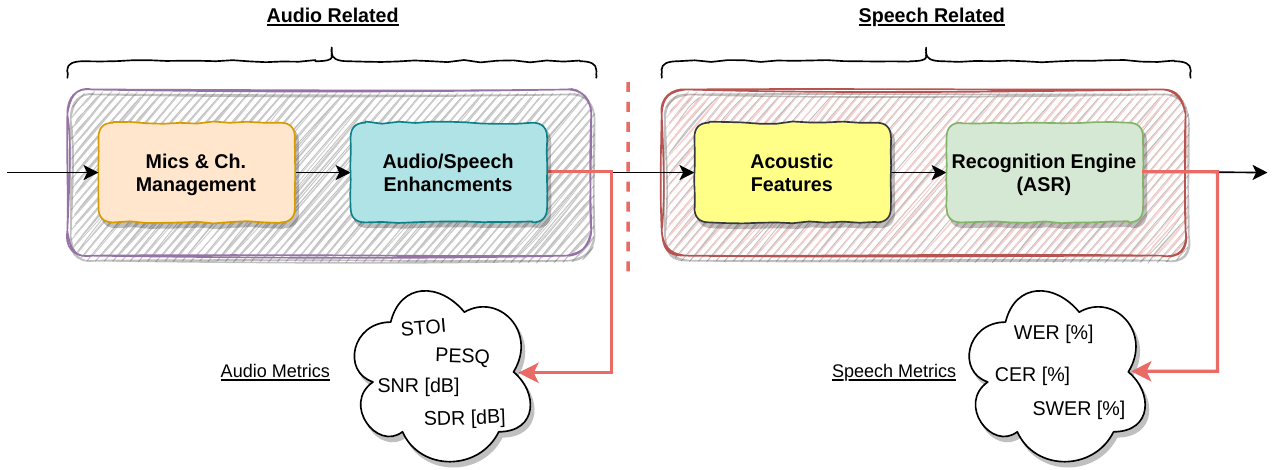
\includegraphics[width=\linewidth]{Introduction/images/asr_blocks}
	\caption{General E2E ASR System Blocks Diagram}\label{fig:asr_blocks_diagram}
\end{figure}
% \begin{figure}[H]
% 	\centering
% 	\includegraphics[width=0.99\textwidth]
% 	{./images/asr_blocks}
% 	\caption{General E2E ASR System Blocks Diagram}\label{fig:asr_blocks_diagram}
% \end{figure}
\vspace{-0.5cm}

% Notwithstanding the acknowledgment that 
% the name references describe each domain's 
% primary intention, they actually overlap.
% Therefore, ``Audio-related'' and ``Speech-related'' are more precise.
% Figure~\ref{fig:asr_blocks_diagram} shows what an End-to-End ASR system is
% generally constructed of. In addition, there is a non-strict distinction between
% two extensive areas in themselves. 


% Although overlap exists between the two domains,
The distinction between the two is characterized
by different metrics.
Typically, speech-recognition performance is evaluated
using the Word Error Rate (WER) and
Character Error Rate (CER) metrics.
On the other hand, audio-related performance,
measured on the enhanced version of the input signal,
whether it be speech separated or noise suppressed,
is evaluated using different metrics.
If such audio enhancement processing is applied,
metrics like Clarity\cite{c50}, Definition\cite{c50d50t50},
Reverberation-Time\cite{c50d50t50}, and other standard signal processing metrics
such as Signal to Noise Ratio (SNR) 
and Signal to Distortion Ratio (SDR) are used.

% Although there is a kind of distinction between these two domains of interest, sometimes the
% distinction line is not strongly put between the ``speech enhancements'' to the ``acoustic features''
% building blocks, nor the requirement to have all these components in an E2E ASR system.

% \bigskip

% With that said, it is still very important
% to distinguish between the different metrics
% that are used to evaluate the performance of such systems. Where speech-recognition related 
% performance is mostly evaluated using the Word Error Rate (WER) and Phone Error Rate (PER) metrics.

% \bigskip

% On the other hand, audio related performance,
% which is measured on the ``enhanced'' version
% of the input signal (if such processing is applied),
% is evaluated using different metrics like 
% Clarity (C50), Definition (D50), Reverberation-Time (T50) 
% and other common signal processing metrics
% as Signal to Noise Ratio (SNR) and Signal to Distortion Ratio (SDR).

\bigskip

In turn, the first building block of the 
``Audio-related'' part that is called 
"Microphones \& Channels Management" as shown 
in Figure~\ref{fig:asr_blocks_diagram},
can be evaluated with 
different sets of performance metrics 
such as Directivity Factor (DF),
Noise Gain (NG) and more.

Compared to a reference and a specific performance metric, 
a change in any of the building blocks 
shown in Figure~\ref{fig:asr_blocks_diagram} may 
improve or degrade performance. 
On the other hand,
performance increase in one metric can cause 
a degradation in other metrics.
Hence, there is a great need 
to perform cross-correlation and trade-off estimations 
over the given metric constraints 
before and during the design stage of an E2E ASR system. 
The outcomes can help in advancing a better approach
which may be a promising solution for a given use case. 
Furthermore, other performance metrics can be examined.
For example, metrics like computation time and resources utilization
can assist in having a more comprehensive overview of how the system operates given a
static pipeline with different algorithms.
Thus, application
developers can benefit from such metrics estimations,
especially when dealing with strict 
application requirements or resource-limited platforms.
% \bigskip

% With the introduction of DNN algorithms,
% E2E ASR systems performance significantly improved
% compared to the conventional HMM-GMM 
% based speech recognition approach\cite{7472778, 6296526}.
% In addition, integration with deep beamformers,
% which are also DNN-based, improves
% the front-end performance in a way that is
% eventually projected to lower WER results.

% \bigskip

% Different neural network (NN) 
% architectures can be used to
% implement of ASR engine building blocks.
% Usually, the NN used to train the ASR engine 
% is the same NN used
% in the implementation of the
% front-end components, microphones, channel management,
% and beamformers.

% in the implementation of the front-end components 
% the same NN is used in the front-end components, Microphones, channel management, and beamformers.

% Different neural network architectures can be applied for
% both the recognition engine, i.e. ASR building block,
% and the front-end components, i.e. Microphones, channel management, and beamformers.

\bigskip

% Compared to a reference and a specific performance metric, 
% each change might improve performance. 
% On the other hand,
% performance in one metric can cause degradation in other metrics.
% Hence, some cross-correlation and trade-off estimations
% should be performed before an E2E ASR system design stage.
% Furthermore, other performance metrics can be embraced.
% For example, metrics like computation time and resources utilization
% can assist in having a more comprehensive overview of how the system operates given a
% static pipeline with different algorithms.
% Thus, application
% developers can benefit from such metrics estimations,
% especially when dealing with strict 
% application requirements or resource-limited platforms.

% when their platforms have limited resources, or when 
% their application requirement are strict.
% for such metrics can be useful for application
% developers, who target for resource limited platforms 
% or are constrained to specific application requirements. 

\section{Literature Review}
References~\cite{7472778, 7952160} are 
two pioneering research papers focusing on 
studying neural networks usages
for beamforming in the front-end,
before the acoustic features extraction and
recognition engine stages in E2E ASR systems.
In both papers, the researchers built their architecture
upon the principles of an E2E ASR pipeline.
Those architectures share a similar baseline but have different
DNN-type beamformers, filters, and ASR engines.
Experiments in ~\cite{7472778, 7952160}
focus on WER performance evaluations to express
the system's capabilities under 
different test-cases and inputs.
Few of the test-cases, for example, are a single microphone 
with single channel input,
a single microphone with multi-channel inputs,
and a microphones array.
% \begin{figure}[H]
% 	\centering
% 	\begin{subfigure}[b]{0.41\textwidth}
% 		\includegraphics[width=\textwidth, keepaspectratio=true]
% 		{./images/gcc_dnn_BF_blocks}
% 		\caption{System Architecture Used In~\cite{7472778}}\label{fig:gcc_dnn_BF_blocks}
% 	\end{subfigure}
% 	\begin{subfigure}[b]{0.55\textwidth}
% 		\includegraphics[width=\textwidth, keepaspectratio=true]
% 		{./images/lstm_BF_blocks}
% 		\caption{System Architecture Used In~\cite{7952160}}\label{fig:lstm_BF_blocks}
% 	\end{subfigure}
% \end{figure}

% \bigskip

% Experiments in ~\cite{7472778, 7952160}
% focus on WER performance evaluations to express
% the system's capabilities under 
% different test-cases and inputs.
% Naming few, a single microphone 
% with single channel input,
% a single microphone with multi-channel inputs,
% and a microphones array.

% \bigskip

\subsection{Recent Work}
Recently, new techniques have been introduced~\cite{900384911,20202222222,9003849,7471664,8466865},
such as
different NN architectures that serve as the basis for
the ASR engines.  
% \begin{itemize}[noitemsep]
% 	\item ASR Engine alternatives
% 	\item biasing
% 	\item Low Latency Beamformers
% 	\item Masking operations
% \end{itemize}

\subsubsection{ASR Engine Alternatives}
Performance comparisons between different recognition
engines are described in~\cite{900384911}. 
The different ASR engines include 
Recurrent neural network-transducer (RNN-T), 
Recurrent neural network-attention encoder decoder (RNN-AED),
and Transformer-AED.
These architectures belong to the right side
of the extended E2E ASR structure shown in 
Figure~\ref{fig:asr_blocks_diagram}, 
also referred to as the
Back-end (BE).
BE engines are complex systems by themselves
and thus can be split into multiple smaller
blocks to ease integration.
Despite being very comprehensive, reference~\cite{900384911} 
concentrates on
the ``Speech related'' domain,
such that the primary metric used for evaluation is WER,
without considering the front-end
effect and its correlation to performance.
In addition, the recognition engines in this paper
do not make use of the 
Listen, Attend, and Spell (LAS)~\cite{7472621}
nor the Connectionist Temporal 
Classification (CTC)~\cite{hannun2017sequence},
which are now considered as integral components in modern 
ASR engines after proving to enhance recognition rates drastically. 
% \bigskip

% In~\cite{900384911}, the primary metric used for evaluation is WER.
% The different ASR engines include 
% Recurrent neural network-transducer (RNN-T), 
% Recurrent neural network-attention encoder decoder (RNN-AED),
% and Transformer-AED.
% These architectures belong to the right side
% of the extended E2E ASR structure shown in 
% Figure~\ref{fig:asr_blocks_diagram}, 
% also referred to as the
% Back-end (BE).
% BE engines are complex systems by themselves
% and thus can be split into multiple smaller
% blocks to ease integration.
% Despite being very comprehensive, this research paper 
% concentrates on
% the ``Speech related'' domain
% without considering the front-end
% effect and its correlation to performance.

\subsubsection{Biasing}
Reference~\cite{20202222222} explores the effect of biasing
on a complete E2E ASR system pipeline. 
First, masking operations were
applied in the frequency domain.
Then, biasing information was fed
into the system in combination with the 
masked frequency output. 
The added biasing information
together with the T-F masking and the beamformer
in the front-end showed a substantial reduction
in error rate detections.

% \begin{figure}[H]
% 	\centering
% 	\includegraphics[width=0.99\textwidth]
% 	{./images/e2e_bias_blocks}
% 	\caption{System Architecture Used In~\cite{20202222222}}\label{fig:e2e_bias_blocks}
% \end{figure}


\subsubsection{Low Latency Beamformers}
Low latency beamformers were studied in~\cite{9003849}.
The research results show 
"audio-related" performance comparisons
as a function of the beamformer type and the number
of microphones in the array.
Moreover, each setup's latency was measured to determine 
its time to process. 
The authors of this paper used
two different datasets for their experiments.
The TIMIT dataset~\cite{timitDS} for the generations of noisy reverberant
inputs to the microphone array and the CHiME 3~\cite{chime3DS} dataset
for ASR evaluations.


\subsubsection{Masking Operations}
Reference paper~\cite{7471664} demonstrates experiments on estimations of spectral masks effects
with neural networks based beamformers.
Two different beamformers,  Generalized Eigenvector (GEV)
and Minimum Variance Distortionless Response (MVDR) were tested with and without Bi-directional Long Short-Term Memory (BLSTM)
spectral masks concerning the Power Spectral Distribution (PSD)
and SNR.
However, this paper does not include an E2E pipeline nor the recognition engine.
In other words, this research focuses on the ``Audio-related'' domain.
Indeed, SNR belongs to the
``Audio-related' metric set rather than the
``Speech-related'' metric set,
as shown in Figure~\ref{fig:asr_blocks_diagram}.
\bigskip

Another comprehensive research 
that studies masking operations
is described in~\cite{8466865}.
In this paper, the architecture does not include
the ASR engine. 
Instead, it mainly deals with the enhanced output signal,
signifying that it is also in the ``Audio-related'' domain.
However, this research is unique in that
it utilized both the WER and SDR metrics measurements
for different engines that were plugged in at the BE stage.

% \begin{figure}[H]
% 	\centering
% 	\includegraphics[width=0.75\textwidth]
% 	{./images/robust_mask_blocks}
% 	\caption{System Architecture Used In~\cite{8466865}}\label{fig:robust_mask_blocks}
% \end{figure}

% Here, the engine is not present in the architecture, but only the enhanced 
% output signal which is also in the ``Audio related'' domain.

\section{Project Outline}
Applications have requirements and limitations
that are dictated by their platform or available hardware.
A way to estimate Hardware (HW) requirements for speech
applications based on speech-related or audio-related metric sets
can be helpful to developers of such platforms.
Therefore, optimizations of a given E2E ASR architecture by careful
trade-off selections can lead to more robust and rapidly
developed applications or setups.
That is a significant advance towards fast setup constructions for different HW platforms.
As such, in this thesis, the effects of changing different
building blocks and applying various enhancement techniques
in a given E2E ASR system will be evaluated.
The effects of such replacements and
fine-tunes will be presented with respect to different
performance metrics. Based on the results, one will be able to deduce the trade-offs
that can be selected to optimize the implementation process for a specific
application, platform, requirement, feasibility, and other specifications.

\bigskip

Evaluated performance metrics
are shown in Figure~\ref{fig:metrics_cross_blocks}
% , where the goals of the research are
% to produce a cross-correlation between the different
% metric sets and trade-offs that can be used to select an optimal design.

\begin{figure}[H]
    \centering
    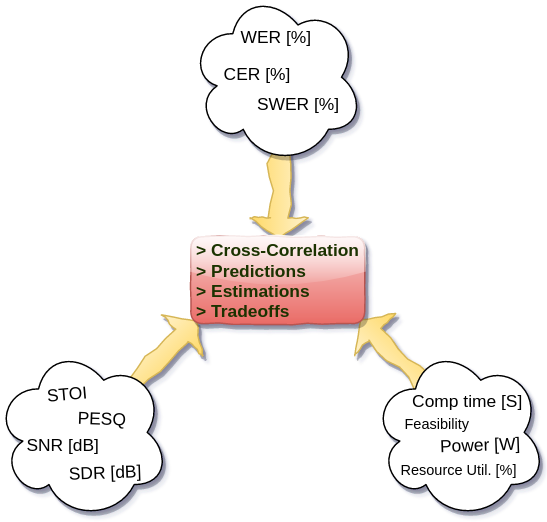
\includegraphics[width=0.75\linewidth]{Introduction/images/metrics_cross_blocks}
    \caption{Project Outline Summary Diagram}\label{fig:metrics_cross_blocks}
\end{figure}
% \begin{figure}[H]
% 	\centering
% 	\includegraphics[width=0.7\textwidth]
% 	{./images/metrics_cross_blocks}
% 	\caption{Project Outline Summary Diagram}\label{fig:metrics_cross_blocks}
% \end{figure}

A comprehensive performance metrics table that contains the Audio,
Speech, and HW characteristics
of an E2E ASR system, will be composed.
Such tables make it easier to detect cross-correlations between the metric sets.
In consequence, 
deduction of each metric's
projection on others can be estimated.

% Hardware metrics estimations based on the other metric sets
% can be useful for application developers. Usually applications have requirements 
% and limitations that are constrained to their platform or available hardware.
% Therefore, some trade-offs

% \bigskip


% that can be selected in order to optimize a given E2E ASR
% architecture can lead to more robust and rapidly developed applications or setups.
% That is a big advance towards fast setup constructions for different hardware platforms. 


% In this research project, I want to study the effects as described in the project outline section.
Our approach is to setup an architecture 
that follows the entire E2E ASR pipeline including
the beamforming FE as presented in
Figure~\ref{fig:proj_blocks}.
% but also includes 
% masking operations 
% Figure~\ref{fig:e2e_bias_blocks}, with some changes that will be described below. 
% The system should follow the baseline pipeline as shown in 
% Figure~\ref{fig:gcc_dnn_BF_blocks} and Figure~\ref{fig:lstm_BF_blocks}.
\begin{figure}[H]
	\vspace{-2.65cm}
	\centering
	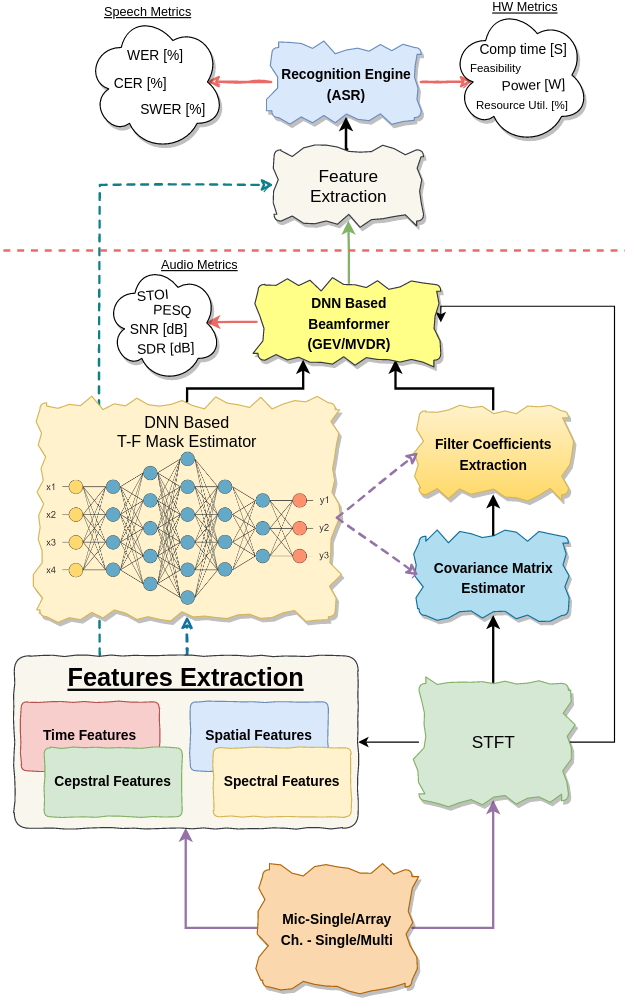
\includegraphics[width=\textwidth]
	{Introduction/images/proj_blocks2}
	\caption{Project Architecture}\label{fig:proj_blocks}
\end{figure}



This paper's structure follows the architecture
presented in Figure~\ref{fig:proj_blocks}.
In Chapter~\ref{ch:metrics}, 
we introduce the selected performance evaluation metrics
of interest and how they relate to these domains. 
A detailed explanation of how each performance metric is
extracted and calculated is provided as well
for a better understanding of the motivation behind
these metrics selection.

Chapter~\ref{ch:scaling_methods} describes three different scaling methods
that are commonly used in audio processing and analysis.
We also present detailed performance comparisons in this chapter based on
the evaluation metrics that we described in Chapter~\ref{ch:metrics}.

The understanding of audio frequency scaling and 
the differences between scaling methods
are essential for Chapter~\ref{ch:features}.

In Chapter~\ref{ch:features}, 
presents key aspects of feature analysis 
along with the considerations 
and importance of every feature.
We conclude that chapter indicating 
that a wise feature selection 
is essential for the sake of 
accurate speech classification and audio processing. 

Chapter~\ref{ch:tf_mask_ch} surrounds Time-Frequency (TF) 
masking techniques which is a preliminary process taken prior
to beamforming. 
In this chapter, we cover four
dominant masking technique, starting with background theory,
through implemntation to measured performance evalutaions.
The T-F masking outputs are dynamically estimated
by a DNN subsystem 
and serve as the input weights
to a beamformer that is connected next.

Beamforming concepts and 
common beamforming architectures for speech
are described in Chapter~\ref{ch:beamformers}.
This chapter follows the T-F masking chapter
since it actually work on the outputs that are produced
by the T-F masking DNN system.

General background about 
ASR systems is given in
Chapter~\ref{ch:asr_ch}.
We then go through history in the development
of ASR systems to the E2E ASR systems.
We emphasize the benefits of using E2E solutions
and what other advancements were done in this field of research.
Here, we present our general approach of an ASR engine implementation,
followed by multiple variants of 
suggested ASR engines and their measurement evaluations.

Chapter~\ref{ch:datasets} describes the datasets that
we use for training and evaluations of our various
DNN systems. We make use of the multi-microphone CHiME datasets~\cite{chime3DS}
for the T-F masking and beamforming parts, 
and the CommonVoice V7 dataset~\cite{commonVoiceDS}
for the ASR engine module.

In Chapter~\ref{ch:concl_ch}, we state our conclusions for this study
and our plan for future work.
  \cleardoublepage
  \printbibliography[title={References}]
\end{refsection}

\begin{refsection}[Features/metrics_paper_ref.bib]
  \chapter{E2E Evaluation Metrics}
\section{Audio Metrics}
\subsection{SNR - Signal to Noise Ratio}
The signal-to-noise ratio (SNR) metric evaluates how
distinct is the desired signal out of the overall noise.

Let \(y(t)\) denote a mixed time-domain signal consisted of
both the desired speech signal and some inferences, referred as noise.
That mixture is given by:
\begin{align}
    y(t) = x(t) + n(t)
\end{align}

Where \(x(t)\), \(n(t)\) denote the speech signal and the
interference noise respectively.

Ideal speech separation of the mixture is characterized by
a perfect match between the predicted speech signal, \(\widehat{x}(t)\), 
and the original (target) speech signal \(x(t)\).
% Separating the speech out of the mixture,
% the predicted speech signal, \(\widehat{x(t)}\), has to match the
% original (target) speech signal \(x(t)\).

Such a problem can be modeled and optimized by the MSE (L2) loss function as follows:
\begin{align}
    \ell(\widehat{x}, x) & = \sum_{t=0}^{T-1} \left[\widehat{x}(t) - x(t)\right]^{2} \\
    & = \sum_{t=0}^{T-1} |r(t)|^{2}
\end{align}

The term \(\sum_{t} |r(t)|^{2}\) is the total energy of the residual error between 
the predicted signal and the target speech, which translate to noise.

According to Parseval's theorem, the residual energy in time equals the sum of
the power difference between the predicted magnitude and the target speech magnitude
in frequency domain.
\begin{align}
    \sum_{t} |r(t)|^{2} & = \frac{1}{T}\sum_{\tau=0}^{T-1}\sum_{f=0}^{T-1} \left[ \widehat{X}(\tau, f) - X(\tau, f)\right]^{2}
\end{align}

Since the residual energy is referred as the noise, minimizing the residuals, 
or in other words minimizing the MSE loss function, translates into an increase in SNR.
The SNR is therefore given by:
\begin{align}
    SNR & = 10\log_{10} \left( \frac{ \| x\|^{2}}{\|x - \widehat{x}\|^{2}}  \right) \nonumber \\
    & =  10\log_{10} \left( \frac{ \| x \|^{2}}{\| r \|^{2}} \right)
\end{align}
\subsection{SI-SNR Scale Invariant SNR}
To ensure that the SNR is susceptible to scale invariance,
both the target and estimated signals are normalized to zero-mean.

\begin{align}
    SI-SNR & = 10\log_{10} \left( \frac{\left\| x - \mathbf{E}[x]\right\|^{2}}
    {\left\| (x - \mathbf{E}[x]) - (x - \mathbf{E}[\widehat{x}]) \right\|^{2}} \right) \nonumber \\
    & = 10\log_{10} \left( \frac{ \| x_{_{AC}}\|^{2}}{\|x_{_{AC}} - \widehat{x}_{_{AC}}\|^{2}}  \right) \nonumber \\
    & =  10\log_{10} \left( \frac{ \| x_{_{AC}}\|^{2}}{\| r_{_{AC}} \|^{2}} \right)
\end{align}


\subsection{STOI}
\subsection{PESQ}

\section{ASR Metrics}
\subsection{WER}
\subsection{CER}

\section{HW Metrics}
\subsection{Computation time}
\subsection{Utilization Ratio}
\subsection{Power Estimation}
\subsubsection{Internal Power}
\subsubsection{Switching Power}
\subsubsection{Leakage Power}

  \cleardoublepage
  \printbibliography[title={References}]
\end{refsection}

\begin{refsection}[Scaling/scaling.bib]
  \chapter{Audio Frequency Scaling methods}\label{ch:scaling_methods}
\section{Introduction}
The human hearing system can detect 
acoustic vibrations and translate 
those vibrations into sounds.
The detectable range of frequencies by the human ear
is referred to as audio or sonic. This range
spans over approximately \(20kHz\),
starting at \(20Hz\) to about \(20kHz\)
\cite{hearthres}.

As a result of aging, the hearing system's dynamic range 
as to the detectable bandwidth decreases,
and by middle-age are set at about
\(20Hz \div 14KHz\)\cite{Wiley2008ChangesIH}.
That is the maximum hearable frequency
declines with age.

The human ear's ability to distinguish 
between two different frequencies 
is not symmetric. 
For example, the spectral distance between two 
different frequencies in one distinction region does 
not equal the spectral distance 
between two additional frequencies in other distinctive regions.

Therefore, the conventional linear 
spectral mapping is impractical for
speech analysis applications.
Thus, a different spectral mapping 
based on a different scaling system
that mimics the human hearing as possible
is applied as an alternative.

\section{Mel-Scaling}
The Mel-scaling method 
is a suggested solution to mapping 
standard audio frequencies to perceived frequencies.
The basic idea that lies underneath is that for
different pitches, we assign varying bandwidth,
such that they were chosen to be equal in distance
from each other, as rated by listeners.
The reference point has been chosen to be 
\(1000 Hz = 1000 Mels\).

Mel-scale has been described first in \cite{Volkmann} by Stevens and Volkmann.
In \cite{Volkmann}, the authors presented different curves
that best describe the Mel-scaling.

Two common tables were composed
according to those curves. One table by 
Beranek in 1949 \cite{beranek1988acoustical} 
and the second by Umesh et al. in 1999 \cite{UmeshMel}.

The most popular equation that models the Mel-scale
is given by \cite{o1987speech}:

\begin{equation}\label{eq:mel_1}
    Mel = \ln \left( 1 + \frac{f}{700} \right) \cdot \frac{1000}{\ln(1+\frac{1000}{700})} 
\end{equation}

This equation\;[\ref{eq:mel_1}] can be simplified as follows:
\begin{align}
    Mel & = 1127 \ln \left( 1 + \frac{f}{700} \right) \nonumber \\
    Mel & = 2595 \log_{10}\left( 1 + \frac{f}{700} \right)
\end{align}

Then, the reverse equation, converting Mels back to Hz,
can be written as:

\begin{align}
    f[Hz] & = 700 \left( 10^{\frac{Mel}{2595}} -1  \right)
\end{align}

\subsection{Logarithm based Mel scale}
The most popular equation that models the Mel-scale
is given by \cite{o1987speech}:
\begin{equation}
    Mel = \ln \left( 1 + \frac{f}{700} \right) \cdot \frac{1000}{\ln(1+\frac{1000}{700})} 
\end{equation}
This can be simplified as follows:
\begin{align}
    Mel & = 1127 \ln \left( 1 + \frac{f}{700} \right) \nonumber \\
    Mel & = 2595 \log_{10}\left( 1 + \frac{f}{700} \right)
\end{align}
Then, the reverse equation, converting Mels back to Hz,
can be written as:
\begin{align}
    f[Hz] & = 700 \left( 10^{\frac{Mel}{2595}} -1  \right)
\end{align}
These modeling equations became de-facto the default way to
map audio frequencies to Mels.

\subsection{Mel scale approximations}

However, computing a logarithm for hardware devices, 
whether it is the natural logarithm or any other base, 
is not very straightforward.
For example, this kind of computation might require special
techniques or long LUTs (look-up tables),
which are extraordinarily resource hungry.

Instead, other approximations that do not involve
trigonometric or logarithms, but only
simple arithmetic structures can be applied.
By doing so, we benefit from low resource
utilization while maintaining high accuracy.

Multiple approximation methods were studied in \cite{fitmelscale}.
Two approximations are the most prominent for target HW devices.
\begin{align}
    \label{eq:melapproxa} Mel & = a + b \cdot f \\ 
    Mel & = \frac{f}{a \cdot f + b} \label{eq:melapproxb}
\end{align}

Where \(a\), \(b\) in Equation \ref{eq:melapproxa} are defined as follows:
\begin{align}
    a & = \begin{cases}
        127.7   &,\;f \leq 1000 \\
        1322    &,\;f > 1000
    \end{cases} \nonumber \\
    b & = \begin{cases}
        0.9     &,\;f \leq 1000 \\
        0.19    &,\;f > 1000
    \end{cases}
\end{align}

while in Equation \ref{eq:melapproxb} \(a\), \(b\) are:
\begin{align}
    a & = \begin{cases}
        0.000244   &,\;f \leq 1000 \\
        0.0004    &,\;f > 1000
    \end{cases} \nonumber \\
    b & = \begin{cases}
        0.741   &,\;f \leq 1000 \\
        0.603   &,\;f > 1000
    \end{cases}
\end{align}

\begin{figure}[H]
    \centering
    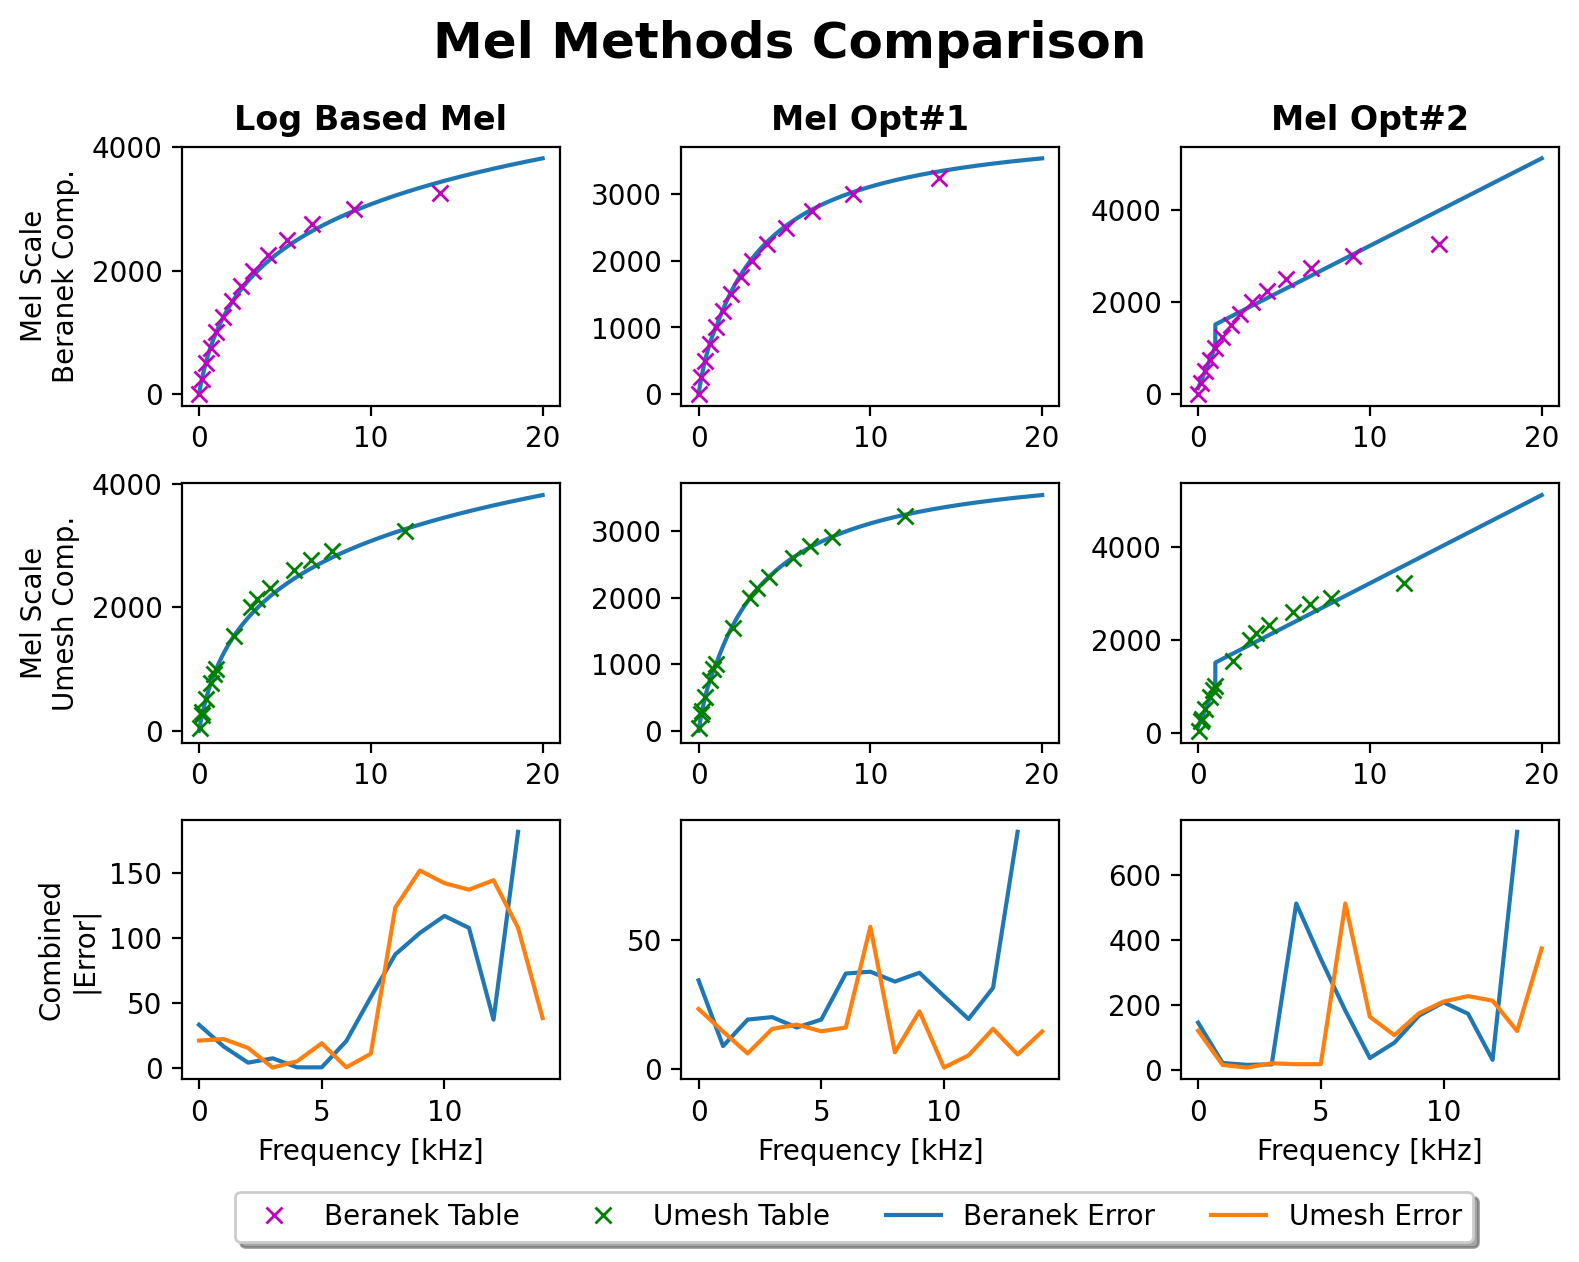
\includegraphics[width=\linewidth]{Scaling/images/mel_methods_comp}
    \caption{Mel scale comparisons with Beranek \& Umesh tables}\label{fig:mel_methods_comp}
\end{figure}

In Figure \ref{fig:mel_methods_comp}, each Mel scaling implementation is than 
the tables suggested by Beranek \& Umesh, respectively. The first column represents
O'Shaugnessy's famous log-based Mel modeling.
The second and third columns follow the suggested approximations
given in Equations \ref{eq:melapproxb} and \ref{eq:melapproxa}, respectively.


From the last row of graphs, we can deduce that the approximation
in Equation \ref{eq:melapproxb} is the closest along with the range of audio frequencies
to the tables provided by Beranek \& Umesh. Saying that, the more simplified 
approximation seems to yield high margins of error.

\begin{figure}[H]
    \centering
    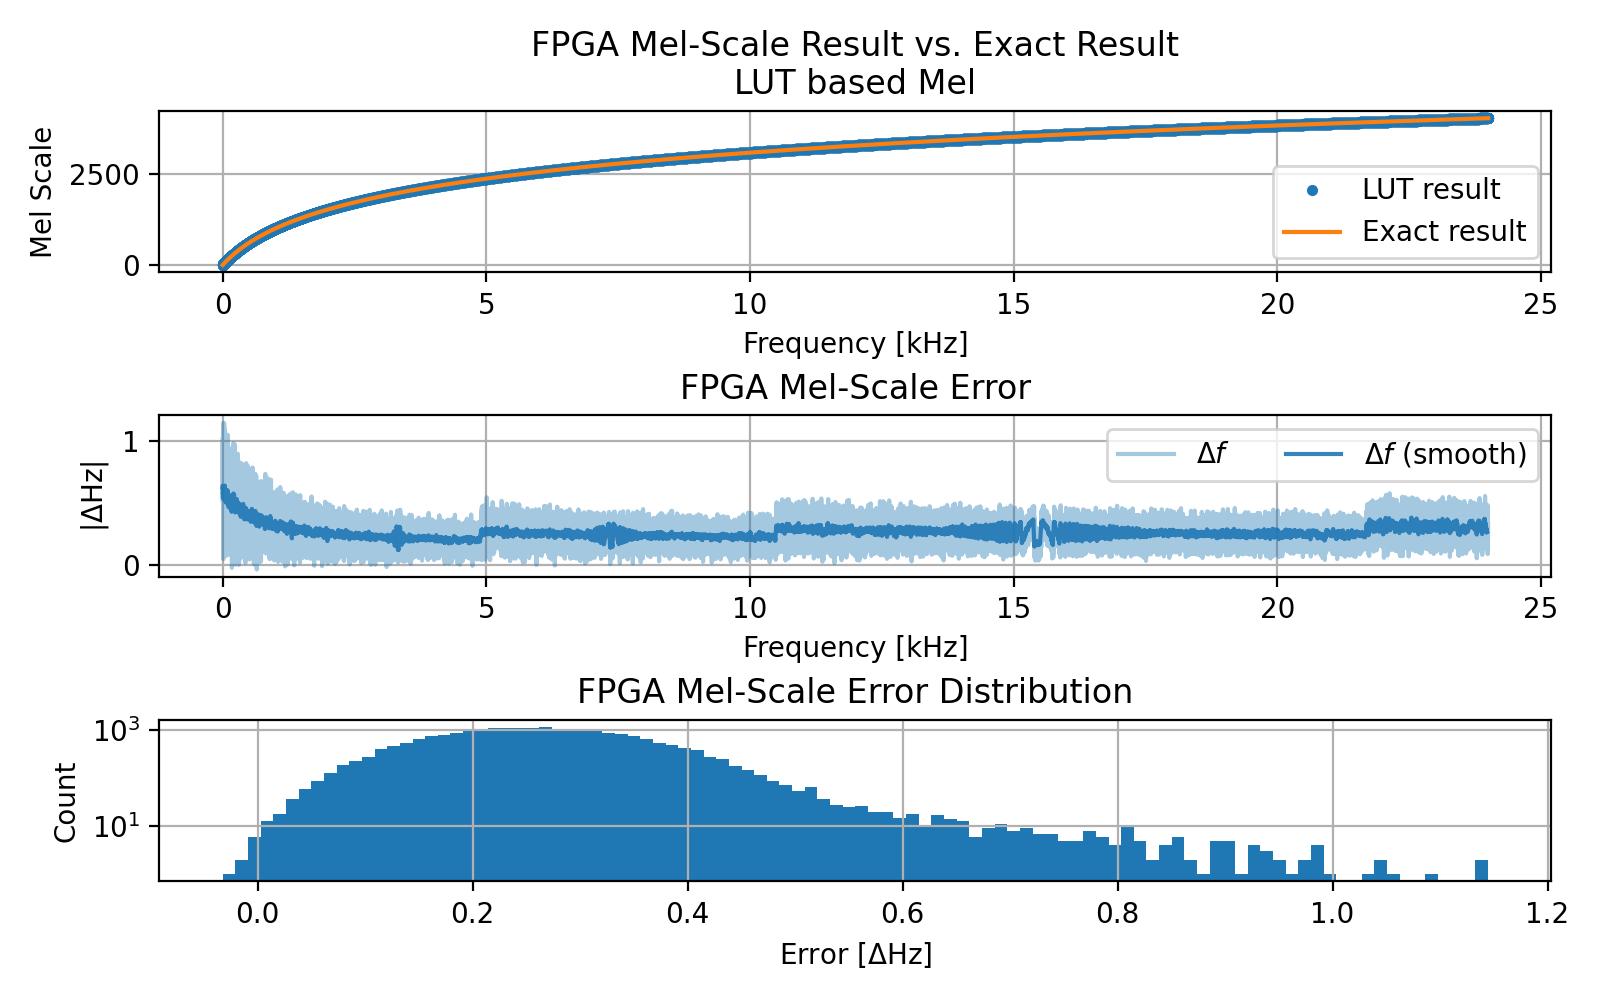
\includegraphics[width=\linewidth]{Scaling/images/mel_lut}
    \caption{LUT based Mel FPGA implementation results}\label{fig:mel_lut}
\end{figure}

\begin{figure}[H]
    \centering
    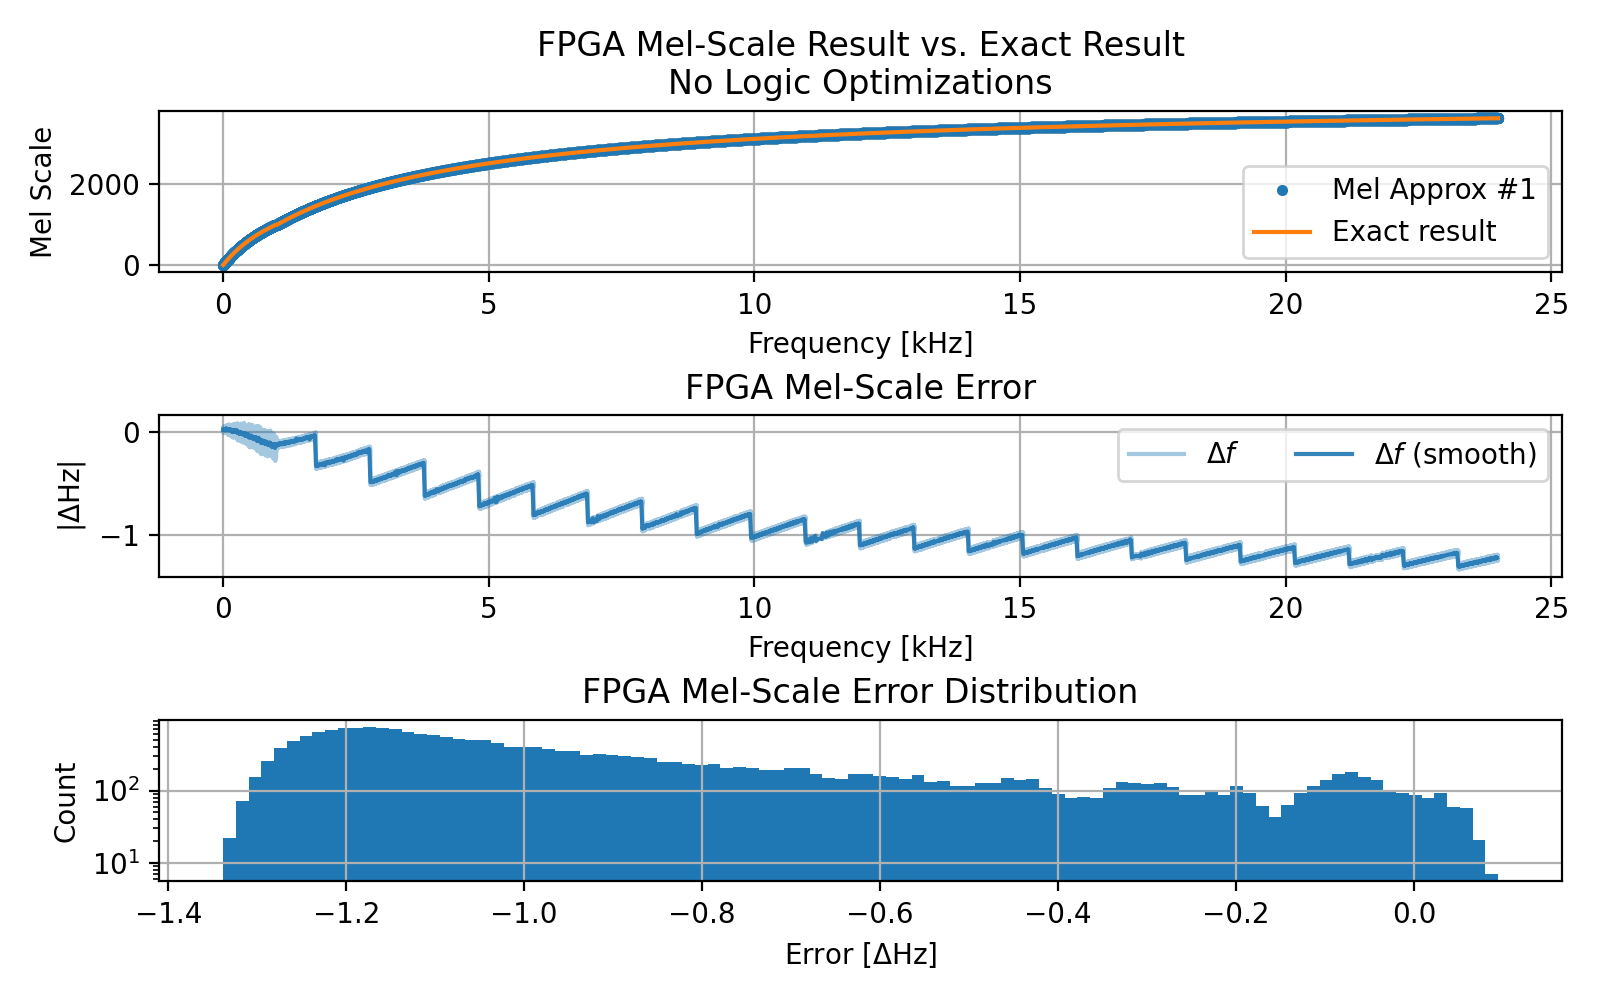
\includegraphics[width=\linewidth]{Scaling/images/mel_approx_no_opt}
    \caption{Mel approx. \#1 FPGA implementation results}\label{fig:mel_approx_no_opt}
\end{figure}

In Figures \ref{fig:mel_lut}, \ref{fig:mel_approx_no_opt} 
presented are the results of FPGA implementations
of O'Shaugnessy's log-based Mel and Mel approximation \#1.
Nonetheless, high precision quantization settings were chosen
for the Mel approximation, U32.22,  
the shifting error received is higher compared 
to the conventional Log Mel scaling implementation.
Although this error shift is compensated 
just by selecting the approximation method, 
the straightforward approach 
turned out to be the non-optimized solution 
in terms of HW resources and power consumption,
which utilized four times higher wattage on top of \(25 \div 30 \%\) 
additional resources.

Instead, two optimization workarounds were tested.
The first is the multiplication of the \(a, b\) coefficients
by 1000. 
The second is reorganizing the equation and storing the 
result in a sufficient precision and lower resolution.  
These optimizations lead to a reduction in the 
required number of bits for the fractional part.
As a result, both the frequency shifting error 
and the overall resources' utilization are greatly improved.
Yet, the split in frequency band results in two multiplied sets
of coefficients for each band calculation.
Therefore, choosing a more generalized set 
of coefficients for the entire audio band can help 
in the reduction of redundant LUTs and other combinational logic, 
such as selectors and multi-bus multiplexer cells.

Selection of \(a=0.24,\;b=0.741\), showed better results
as can be seen in figure \ref{fig:mel_approx_logic_opt_generic}.
The accuracy estimation for the non-generic implementation
is shown in Figure\;\ref{fig:mel_approx_logic_opt}.

\begin{figure}[H]
    \centering
    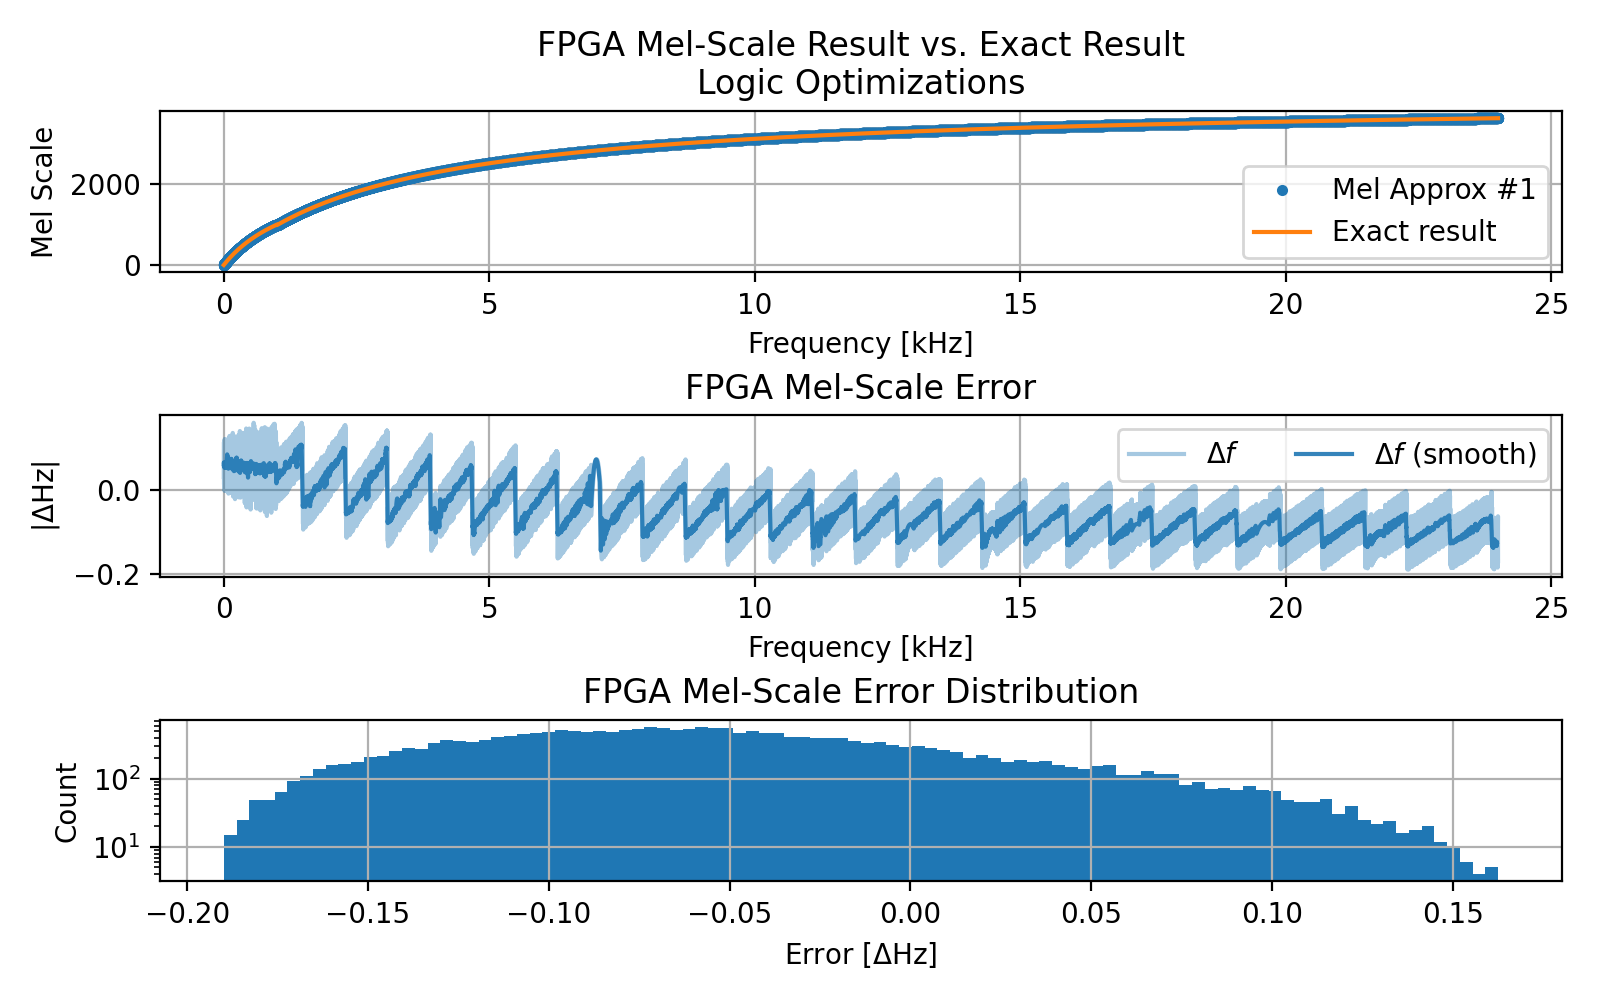
\includegraphics[width=\linewidth]{Scaling/images/mel_approx_logic_opt}
    \caption{Mel approx. \#1 \underline{optimized} FPGA implementation results}\label{fig:mel_approx_logic_opt}
\end{figure}


\begin{figure}[H]
    \centering
    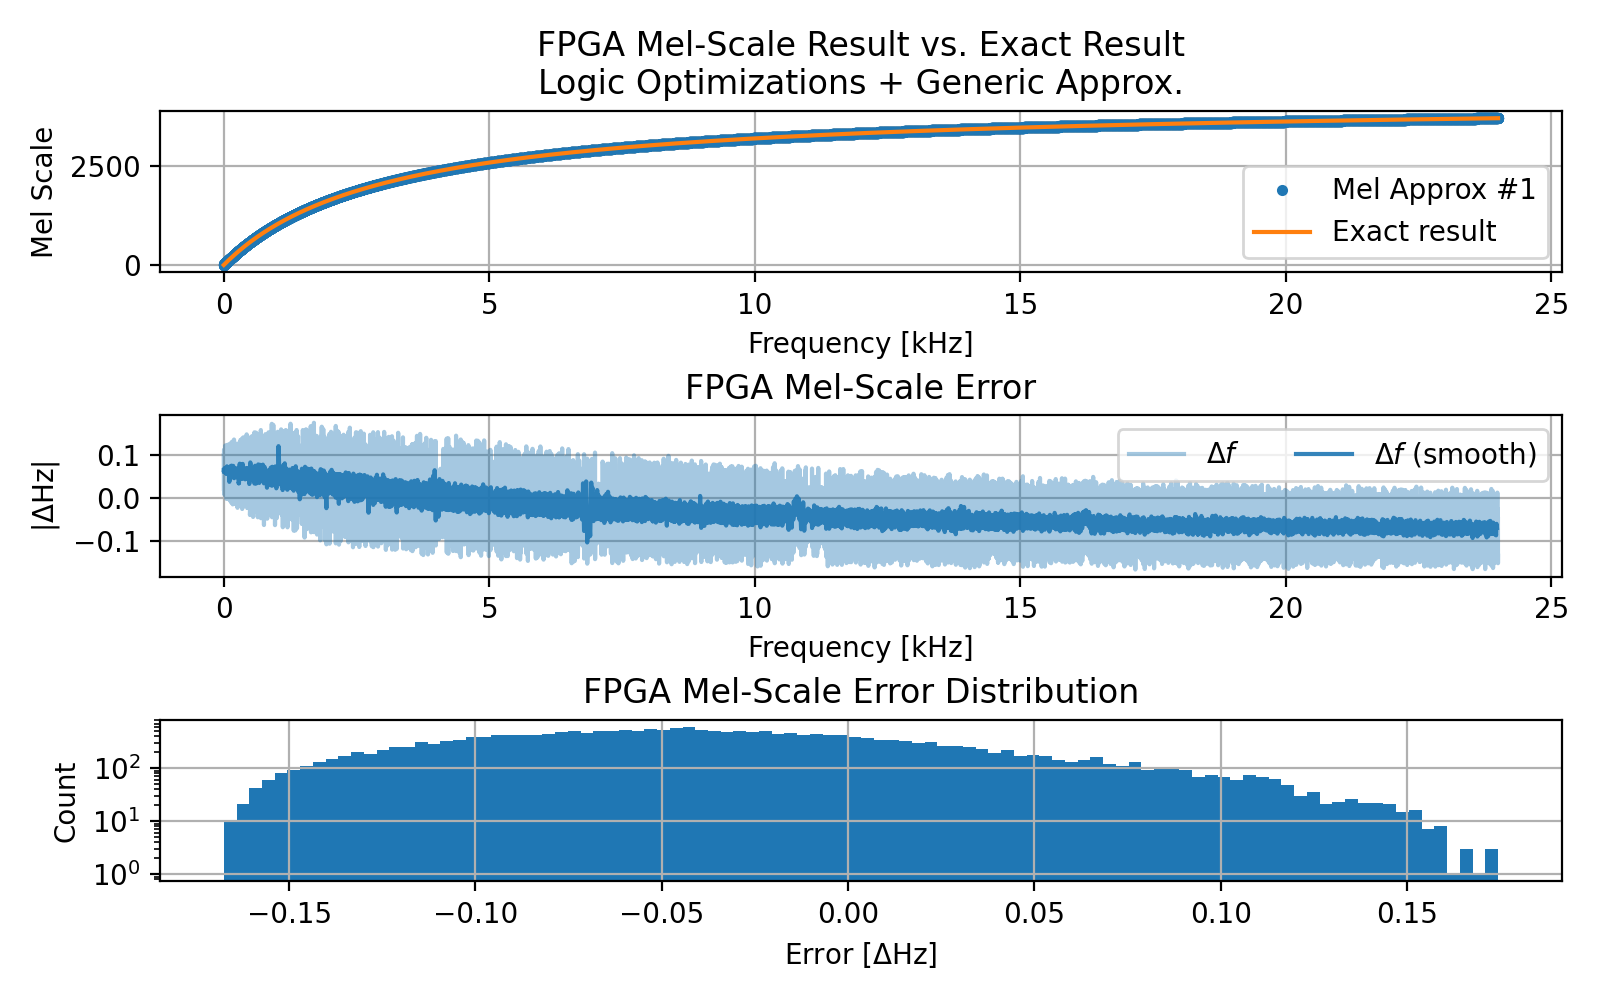
\includegraphics[width=\linewidth]{Scaling/images/mel_approx_logic_opt_generic}
    \caption{Mel approx. \#1 \underline{optimized, generic} FPGA implementation results}\label{fig:mel_approx_logic_opt_generic}
\end{figure}


\begin{table}[H]
    % for more info see: https://www.overleaf.com/learn/latex/tables
    % \centering
    \hspace*{-1.8cm}
    \arrayrulecolor{mtblborder}
\begin{tabular}{ !{\color{mtblborder}\vrule}l!{\color{mtblborder}\vrule}rcccc| } 
    \hline

    \hline
    \rowcolor{mtblcaption} \color{white}\bf{Algorithm} 
    & \color{white}\bf{Latency \([ns]\)}  
    & \color{white}\bf{Quant.} 
    & \color{white}\bf{Max Err. \([\Delta Hz]\)}
    & \color{white}\bf{Mean Err.}
    & \color{white}\bf{Std Err.} \\
    \hline

    \hline
    \rowcolor{mtbl} Log LUT Mel   & \(14\) (3 C.C) & U16/4 & 1.146 & 0.268 & 0.106 \\
    \hline
    
    \hline
    \rowcolor{wtbl} Mel \#1   & \(9\) (2 C.C) &  U32/22  & 1.338 & -0.873 & -0.359 \\
    \hline
    
    \hline
    \rowcolor{mtbl} Mel \#1 Opt      & \(9\) (2 C.C) &  U16/4  & 0.190 & -0.053 & 0.065 \\
    \hline

    \hline
    \rowcolor{wtbl} Mel \#1 Generic     & \(9\) (2 C.C) &  U16/4  & \color{gtblcaption}0.174 & \color{gtblcaption}-0.035 & \color{gtblcaption}0.061 \\
    \hline

    \hline
\end{tabular}
\arrayrulecolor{black}
\caption{Mel-Approx, log-based Mel performance comparison}
\label{tbl:mel_scale_performance}
\end{table}


\begin{table}[H]
    % for more info see: https://www.overleaf.com/learn/latex/tables
    \centering
    \arrayrulecolor{ytblborder}
\begin{tabular}{ !{\color{ytblborder}\vrule}l!{\color{ytblborder}\vrule}rrrrr| } 
    \hline

    \hline
    \rowcolor{ytblcaption} \color{white}\bf{Algorithm} 
    & \color{white}\bf{FF} 
    & \color{white}\bf{LUT} 
    & \color{white}\bf{DSP} 
    & \color{white}\bf{LUTRAM} 
    & \color{white}\bf{BRAM} \\
    % & \color{white}\bf{ORM} 
    % & \color{white}\bf{Clean} \\
    \hline

    \hline
    \rowcolor{ytbl} Log LUT Mel   & 82(0.04\%) & 276(0.23\%) & 1(<1\%) & 10(0.02\%) & 1.5(1.04\%)  \\
    \hline
    
    \hline
    \rowcolor{wtbl} Mel \#1     & 47(0.02\%) & 530(0.45\%) & 1(<1\%) & 0(0\%)  & 0(0\%)    \\
    \hline
    
    \hline
    \rowcolor{ytbl} Mel \#1 Opt      & 47(0.02\%) & 271(0.23\%) & 1(<1\%) & 0(0\%)  & 0(0\%)    \\
    \hline

    \hline
    \rowcolor{wtbl} Mel \#1 Generic     & 47(0.02\%) & 269(0.19\%) & 1(<1\%) & 0(0\%)  & 0(0\%)    \\
    \hline

    \hline
\end{tabular}
\arrayrulecolor{black}
\caption{Mel scaling methods resource utilization table}
\label{tbl:mel_resource_util}
\end{table}



\begin{table}[H]
    % for more info see: https://www.overleaf.com/learn/latex/tables
    \centering
    \arrayrulecolor{gtblborder}
\begin{tabular}{ |l|cccc| } 
    \hline

    \hline
    \rowcolor{gtblcaption} \color{white}\bf{Parameter} 
    & \color{white}\bf{Log LUT Mel} 
    & \color{white}\bf{Mel \#1} 
    & \color{white}\bf{Mel \#1 Opt} 
    & \color{white}\bf{Mel \#1 Generic} \\
    \hline\hline
    \rowcolor{wtbl}\multicolumn{5}{|c|}{\bf{Dynamic Power [W]}}\\
    \hline
    \rowcolor{gtbl} Signals                 & 4.947 & 5.221 & 3.011 & 2.916  \\
    \hline
    
    \hline
    \rowcolor{wtbl} Logic                   & 6.50 & 6.792 & 3.751 & 3.070  \\
    \hline

    \hline
    \rowcolor{gtbl} DSP                     & 0.014 & 0.013 & 0.014  & 0.014 \\
    \hline
    
    \hline
    \rowcolor{wtbl} I/O                     & 18.236 & 26.263 & 7.207  & 6.378 \\
    \hline
    
    \hline
    \rowcolor{gtbl} \(\mathbf{P_{dynmic}}\) & \textbf{29.697} & \textbf{38.290} & \textbf{13.983}  & \textbf{\color{gtblborder}12.379} \\
    \hline

    % \hline
    % \rowcolor{gtbl} Bark Scale      & 56(0.02\%) & 218(\%) & 1(<1\%)   \\
    % % \cline{2-8}
    % % \multirow{-2}{*}{\cellcolor{ytbl}\#1(5)}   & 14.03/17.78 & 27.06 & 13.73 & - & - & - & 7.72 \\ 
    \hline\hline
    \rowcolor{wtbl}\multicolumn{5}{|c|}{\bf{Static Power [W]}}   \\
    \hline

    \hline
    \rowcolor{gtbl} PL Static               & 2.364 & 2.466 & 0.499  & 0.499 \\
    \hline
    
    \hline
    \rowcolor{wtbl} PS Static               & 0.068 & 0.071 & 0.020 & 0.018  \\
    \hline

    \hline
    \rowcolor{gtbl} \(\mathbf{P_{static}}\) & \textbf{2.432} & \textbf{2.537} & \textbf{0.519} & \textbf{\color{gtblborder}0.517}  \\
    \hline

    \hline\hline
    \rowcolor{wtbl}\multicolumn{5}{|c|}{\bf{Total Power [W]}}   \\
    \hline

    \hline
    \rowcolor{gtbl} \(\mathbf{P_{total}}\)  & \textbf{32.13} & \textbf{40.827} & \textbf{14.502} & \textbf{\color{gtblborder}12.896}  \\
    \hline
\end{tabular}
\arrayrulecolor{black}
\caption{Mel-Approx, log-based Mel, Bark Scale Power consumption}
\label{tbl:mel_scale_pwr_tbl}
\end{table}

The LUT implementation makes use of a \(log_{2}\) look-up table.
However, an additional step is 
needed for the natural logarithm or other log bases. 
Since the logarithm bases are constant, 
the LUT result is divided by the \(log_{2}\) of the base,
whether it be the natural base or base ten.
This logarithm bases 
convention is described in Equation\;\ref{eq:log_base_conv}.
\begin{align}\label{eq:log_base_conv}
    \log_{b}(a)  & = \frac{\log_{x}(a)}{\log_{x}(b)}
\end{align}


Table\;\ref{tbl:mel_scale_performance} summarizes
the performance comparison between the different Mel scaling
implementation approaches. 

The HW setup is for the PYNQ-Z1 development board.
Hence, the results are unique to that specific 
HW device and probably change for other 
FPGA devices and development boards.

Latencies were simulated with Xilinx Vivado Suit
for an operating clock frequency of \(225MHz\).
In this operating condition, no timing violations were reported.

Tables\;\ref{tbl:mel_resource_util} and \ref{tbl:mel_scale_pwr_tbl}
show the synthesis and implementation results 
plus the power estimation reports. 
These reports were taken from the Xilinx Vivado Suit application.

\section{Bark-Scaling}
Another scaling method is the bark scale which is based on
the same principle of retaining the same perceptual distances.
The bark scale is divided into critical 
bands corresponding to the critical hearing bands. 
Each band has a bandwidth similar 
to the psychoacoustic band of the corresponding 
``filter'' in the human hearing system 
and is ranked with a unique number.

\subsection{Bark Critical Bands}
Like the Mel scale, several equations were proposed to model best
the Bark scale and its critical bands.

The first method was introduced in \cite{doi:10.1121/1.1908630}.
A proposed approximation to the bark scaling is described in 
\cite{doi:10.1121/1.399849}. This paper also introduces the 
correction of the band boundaries to ensure more 
correctness with the original bark scaling.

Four different equations were proposed to model
the Bark scale.

The first by Zwicker is well described in\cite{1908630} and
is given by the following equation:

% Zwicker Eq
\begin{align}
    Bark & = \tan^{-1}\left\{ 0.00073f \right\} + 3.5 \tan^{-1}\left\{ 
            \left( \frac{f}{7500} \right)^{2}
        \right\}
\end{align}

Another proposed equation by Traunmuller \cite{TraunmullerScale} is:
% Traunmuller Eq + Correction
\begin{align}\label{eq:traunmuller_no_fix}
    Bark & = \frac{26.81f}{1960 + f} - 0.53
\end{align}

\begin{figure}[H]
    \centering
    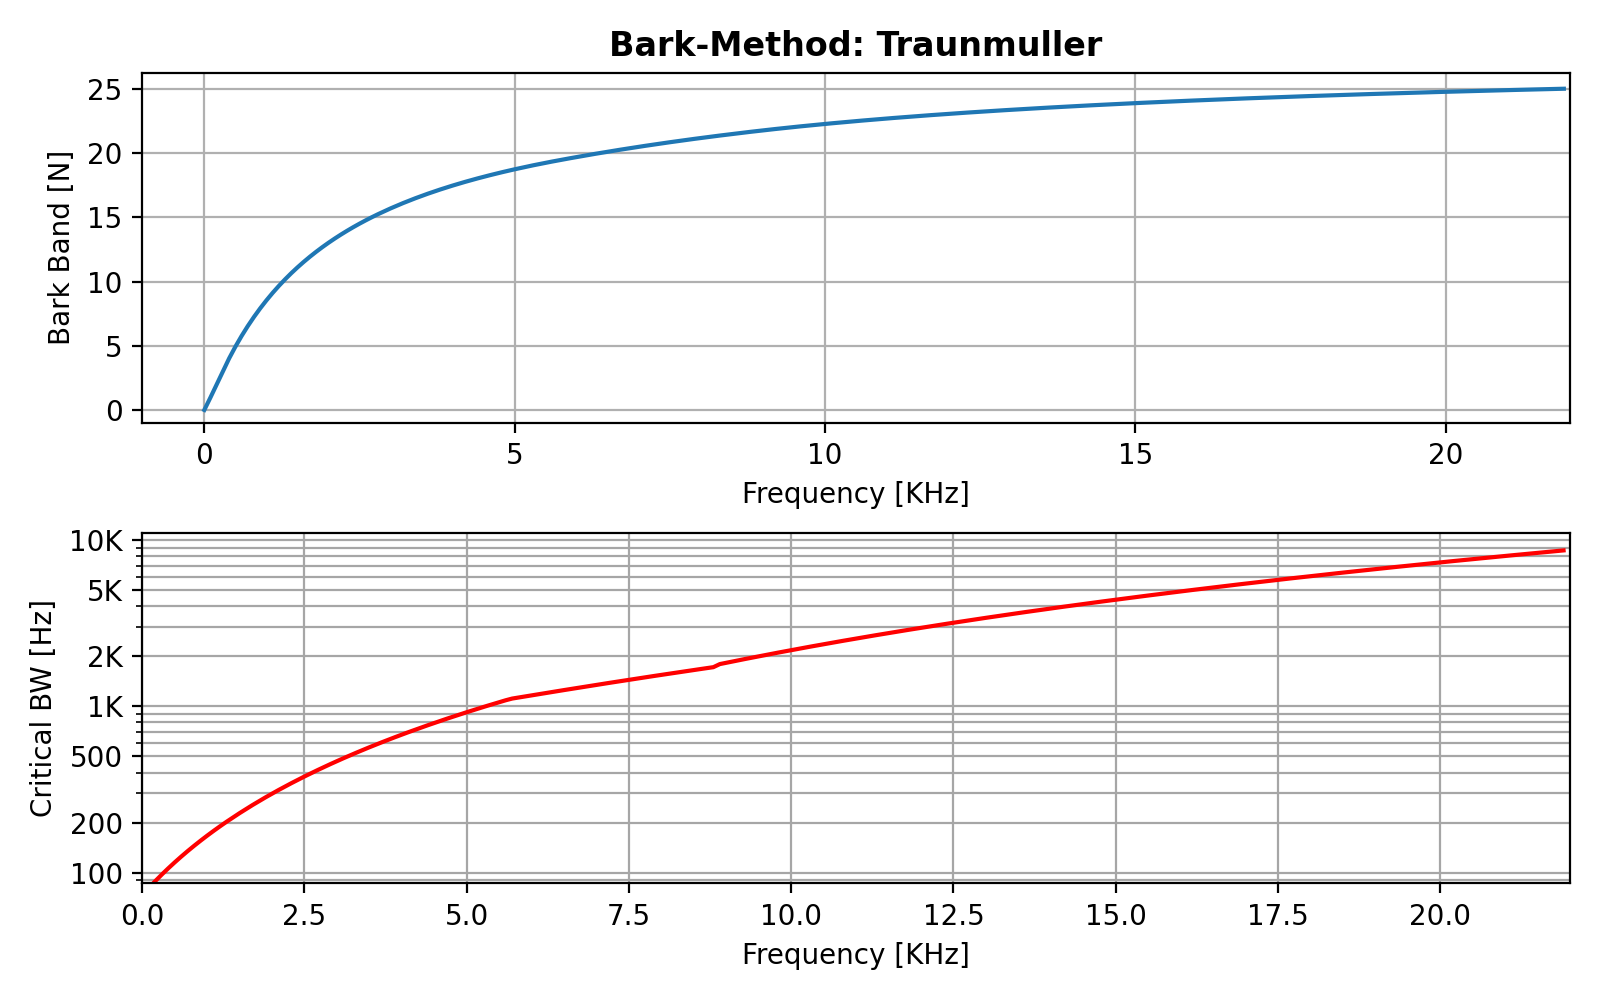
\includegraphics[width=0.75\linewidth]{Experiments/images/Traunmuller_nofix}
    \caption{Traunmuller no fix}\label{fig:Traunmuller_nofix}
\end{figure}

Denoting Traunmuller's original
Bark scale given in Equation \ref{eq:traunmuller_no_fix} as \(Bark'\),
the fixed form for Traunmuller's Bark equation is:
\begin{align}
    Bark & = \begin{cases}
        0.3 + 0.85\cdot \left( Bark' \right) 
        &,\;Bark' < 2 \\
        Bark' + 0.22\cdot \left( Bark' - 20.1 \right) 
        &,\;Bark' > 20.1
    \end{cases}
\end{align}

\begin{figure}[H]
    \centering
    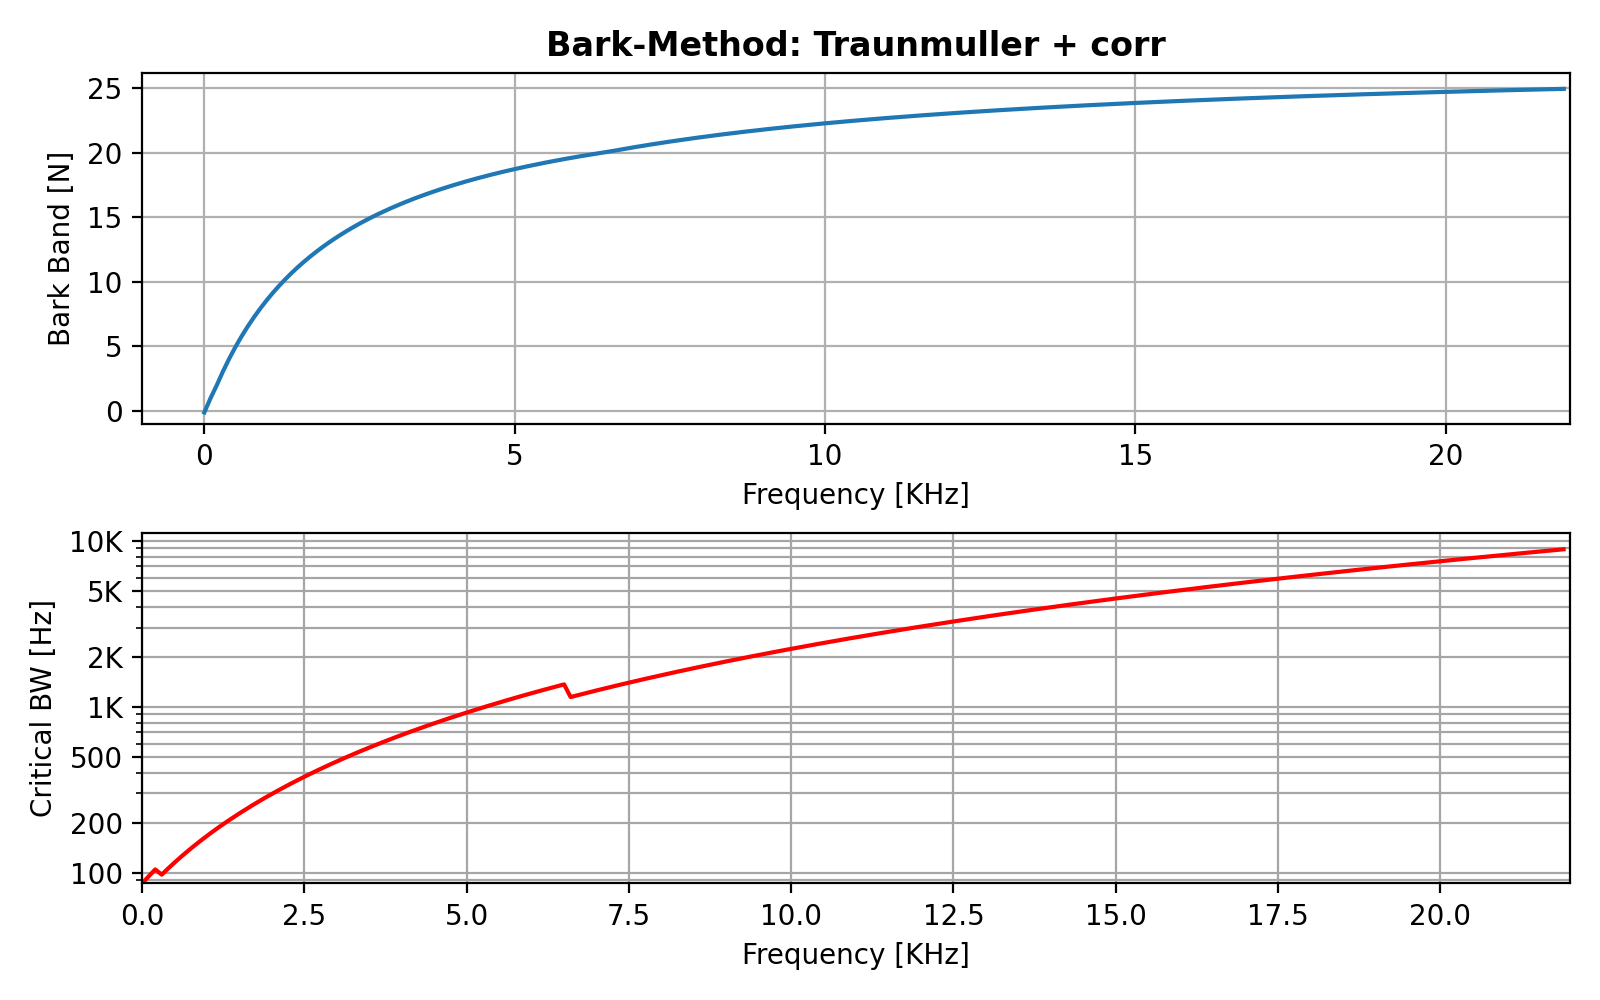
\includegraphics[width=0.75\linewidth]{Experiments/images/Traunmuller_fix}
    \caption{Traunmuller fix}\label{fig:Traunmuller_fix}
\end{figure}

The fourth possible modeling equation is proposed by
Schroeder in \cite{SchroederScale} and is as follows:
% Schroeder Eq
\begin{align}
    Bark & = 7\ln \left( \frac{f}{650} + \sqrt{1 + \frac{f^{2}}{422500} }  \right)
\end{align}


\begin{figure}[H]
    \centering
    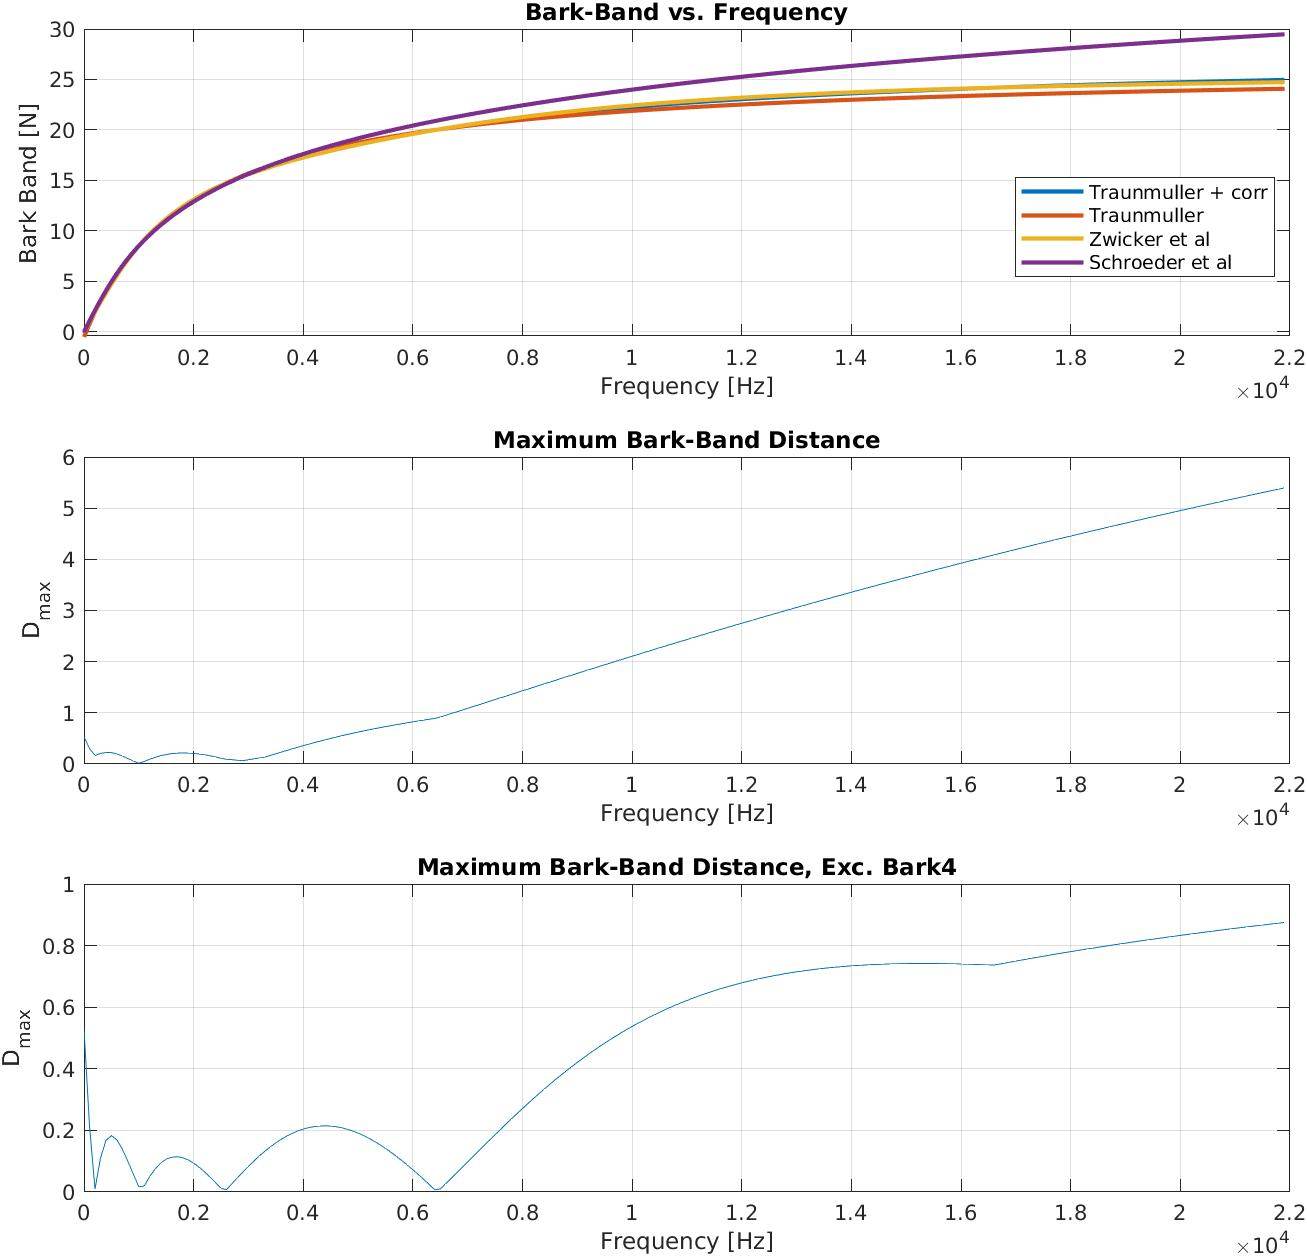
\includegraphics[width=0.75\linewidth]{Experiments/images/bark_comparison}
    \caption{Bark comparisons}\label{fig:bark_comparison}
\end{figure}


\begin{figure}[H]
    \centering
    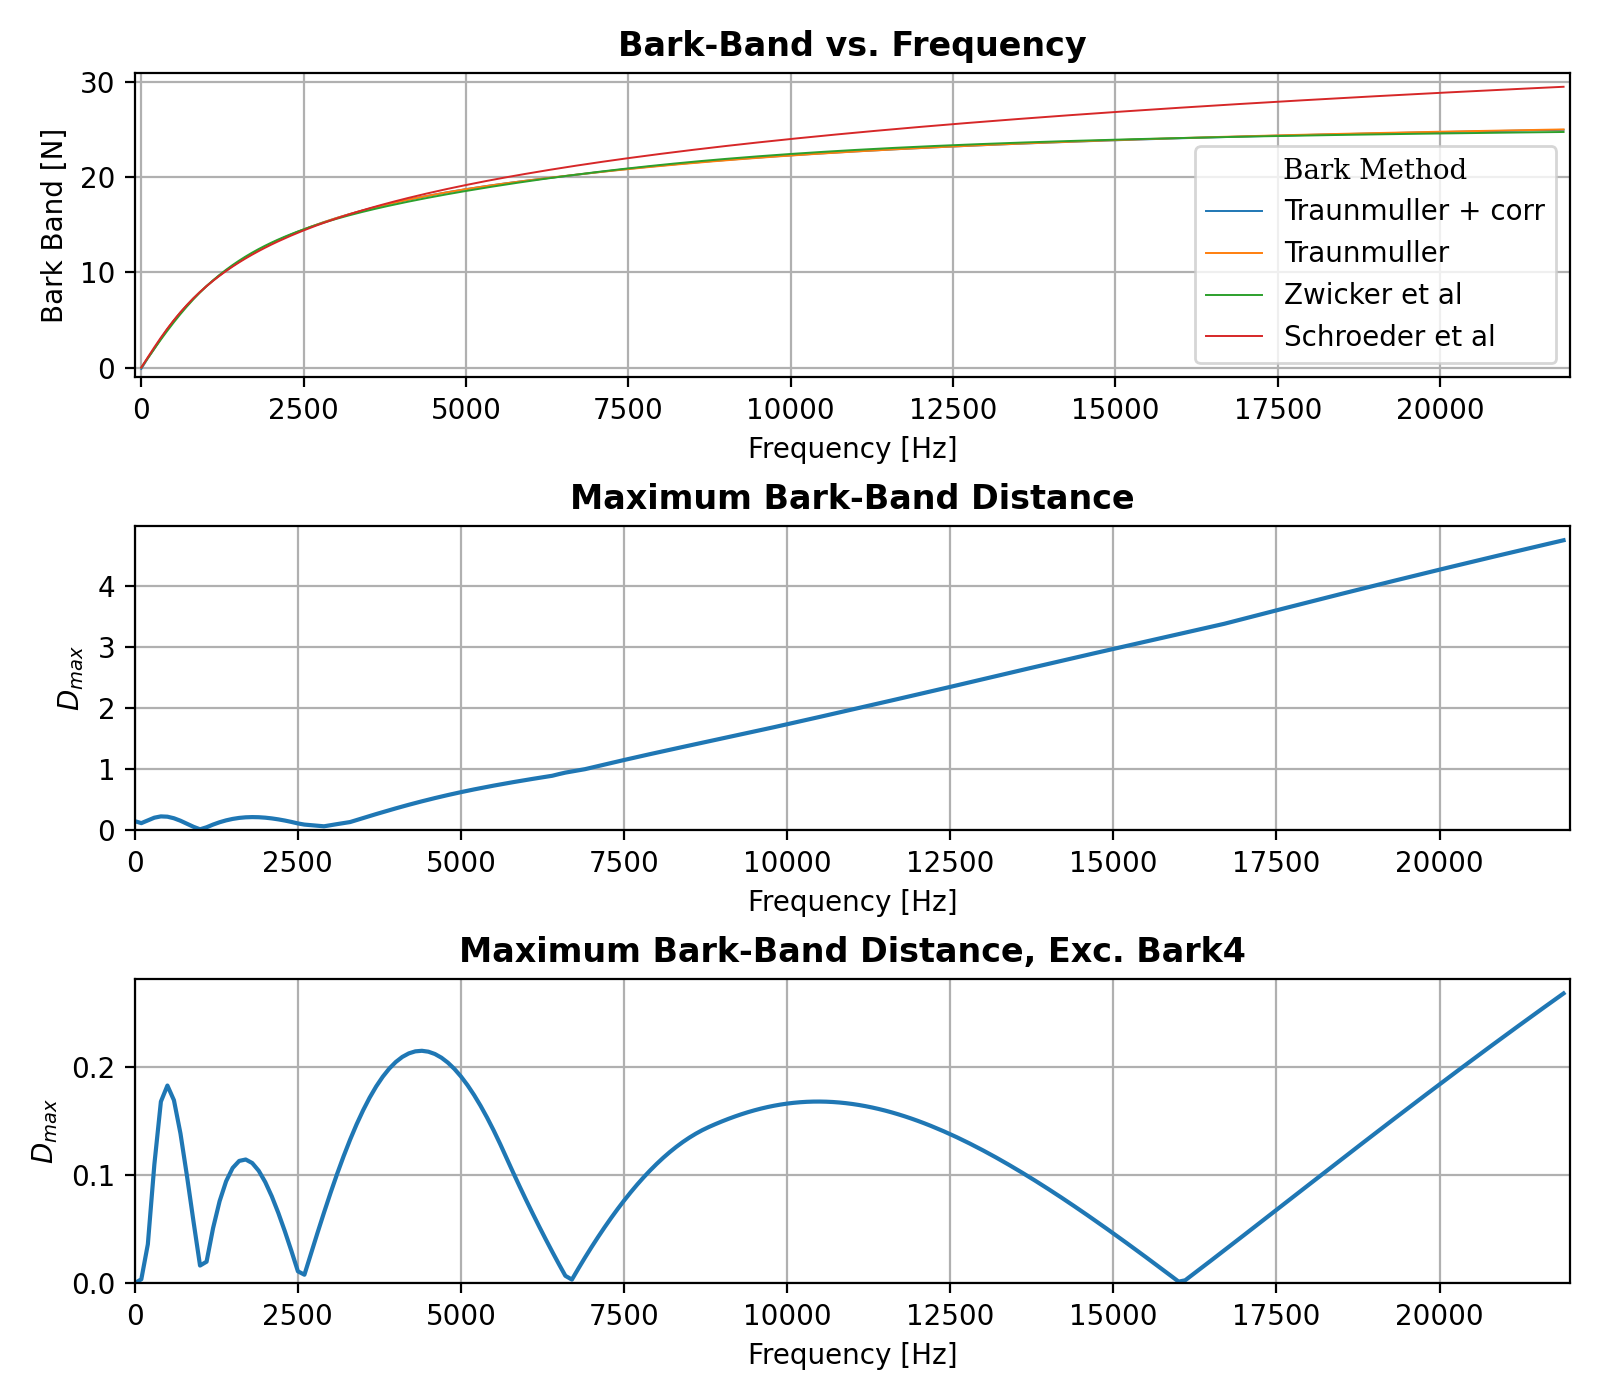
\includegraphics[width=0.75\linewidth]{Experiments/images/bark_comparison2}
    \caption{Bark comparison}\label{fig:wer_23}
\end{figure}



\begin{figure}[H]
    \centering
    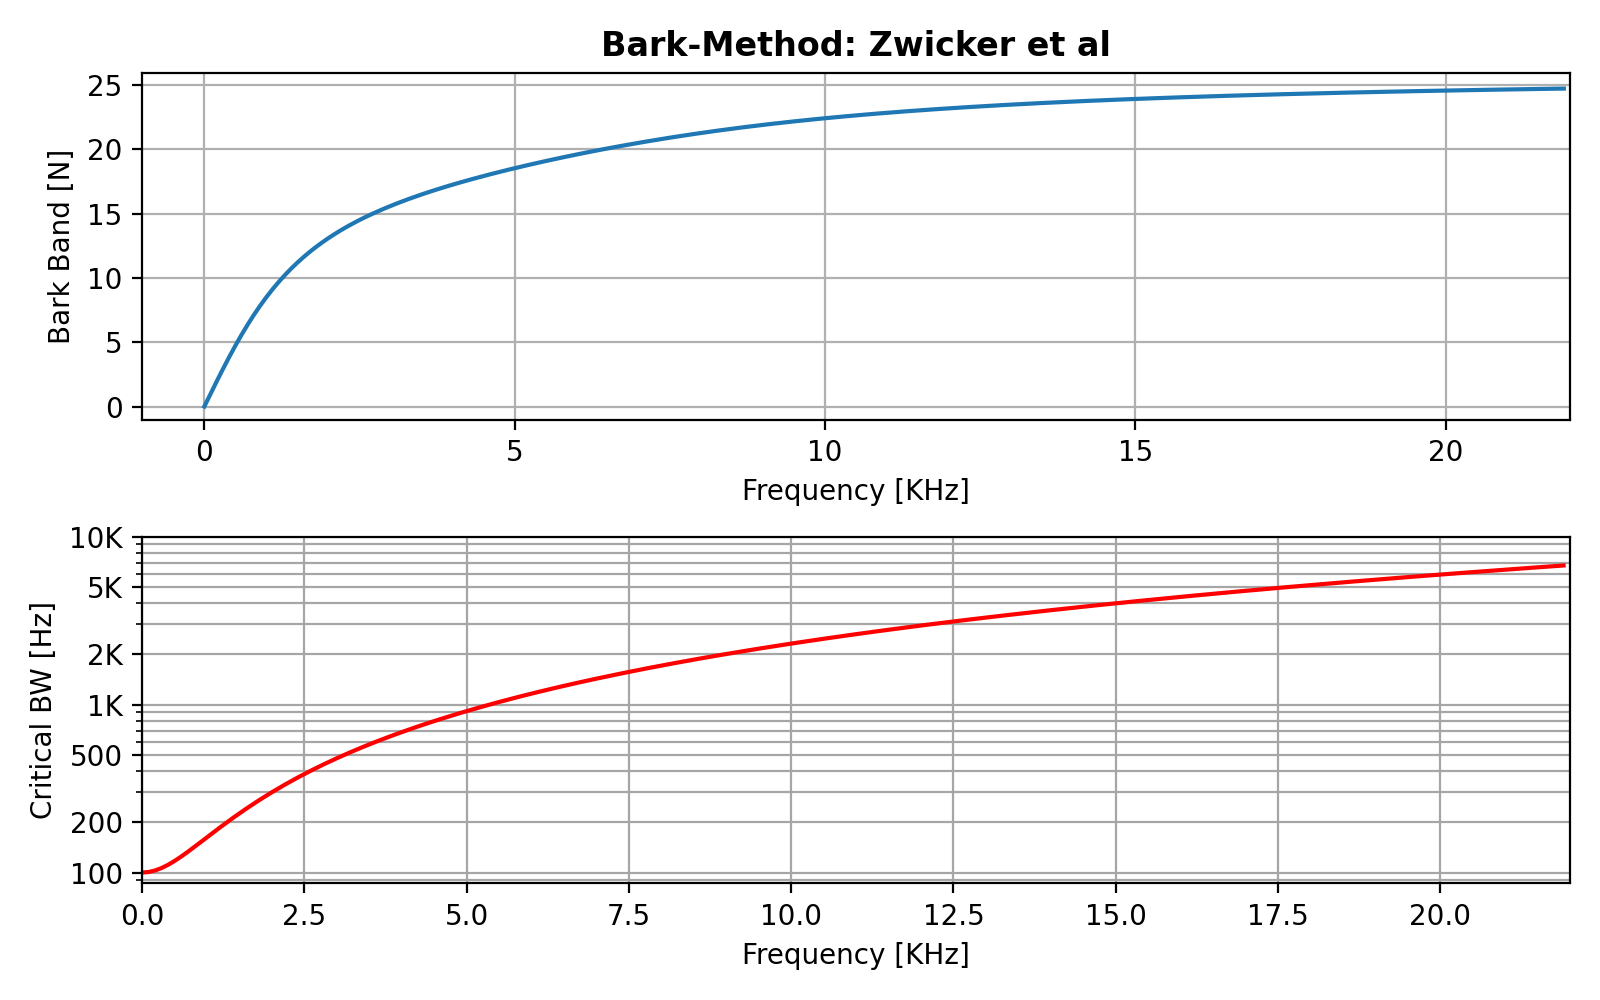
\includegraphics[width=0.75\linewidth]{Experiments/images/Zwicker}
    \caption{Zwicker}\label{fig:Zwicker}
\end{figure}

\begin{figure}[H]
    \centering
    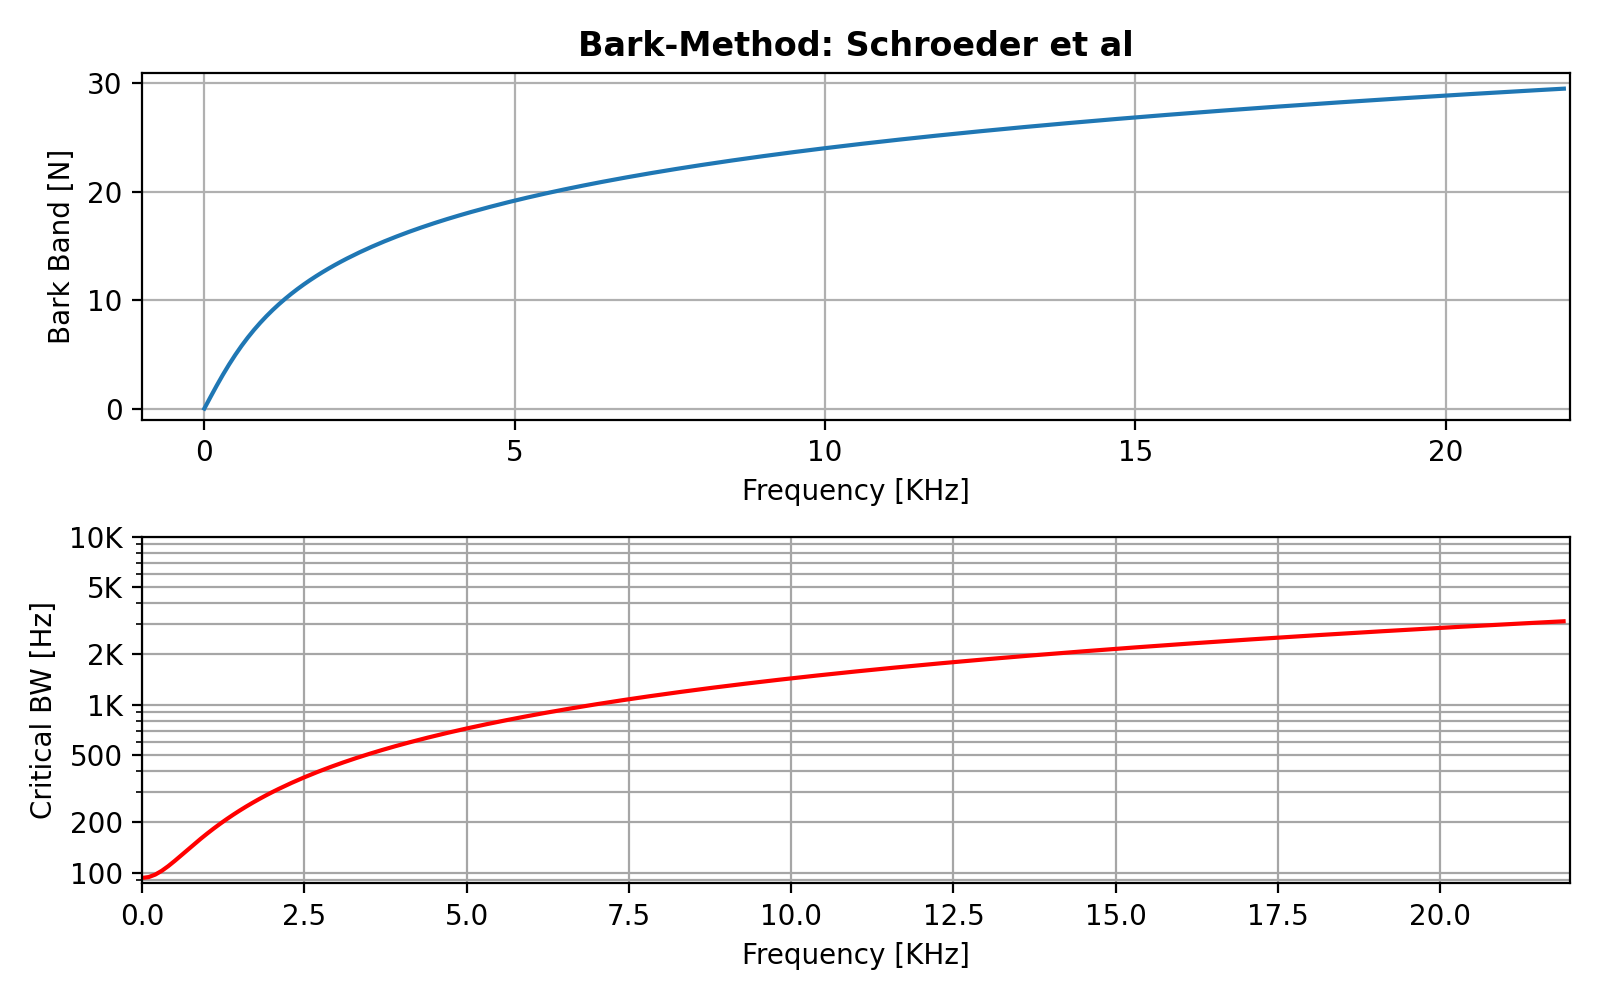
\includegraphics[width=0.75\linewidth]{Experiments/images/Schroeder}
    \caption{Schroeder}\label{fig:Schroeder}
\end{figure}


\begin{figure}[H]
    \centering
    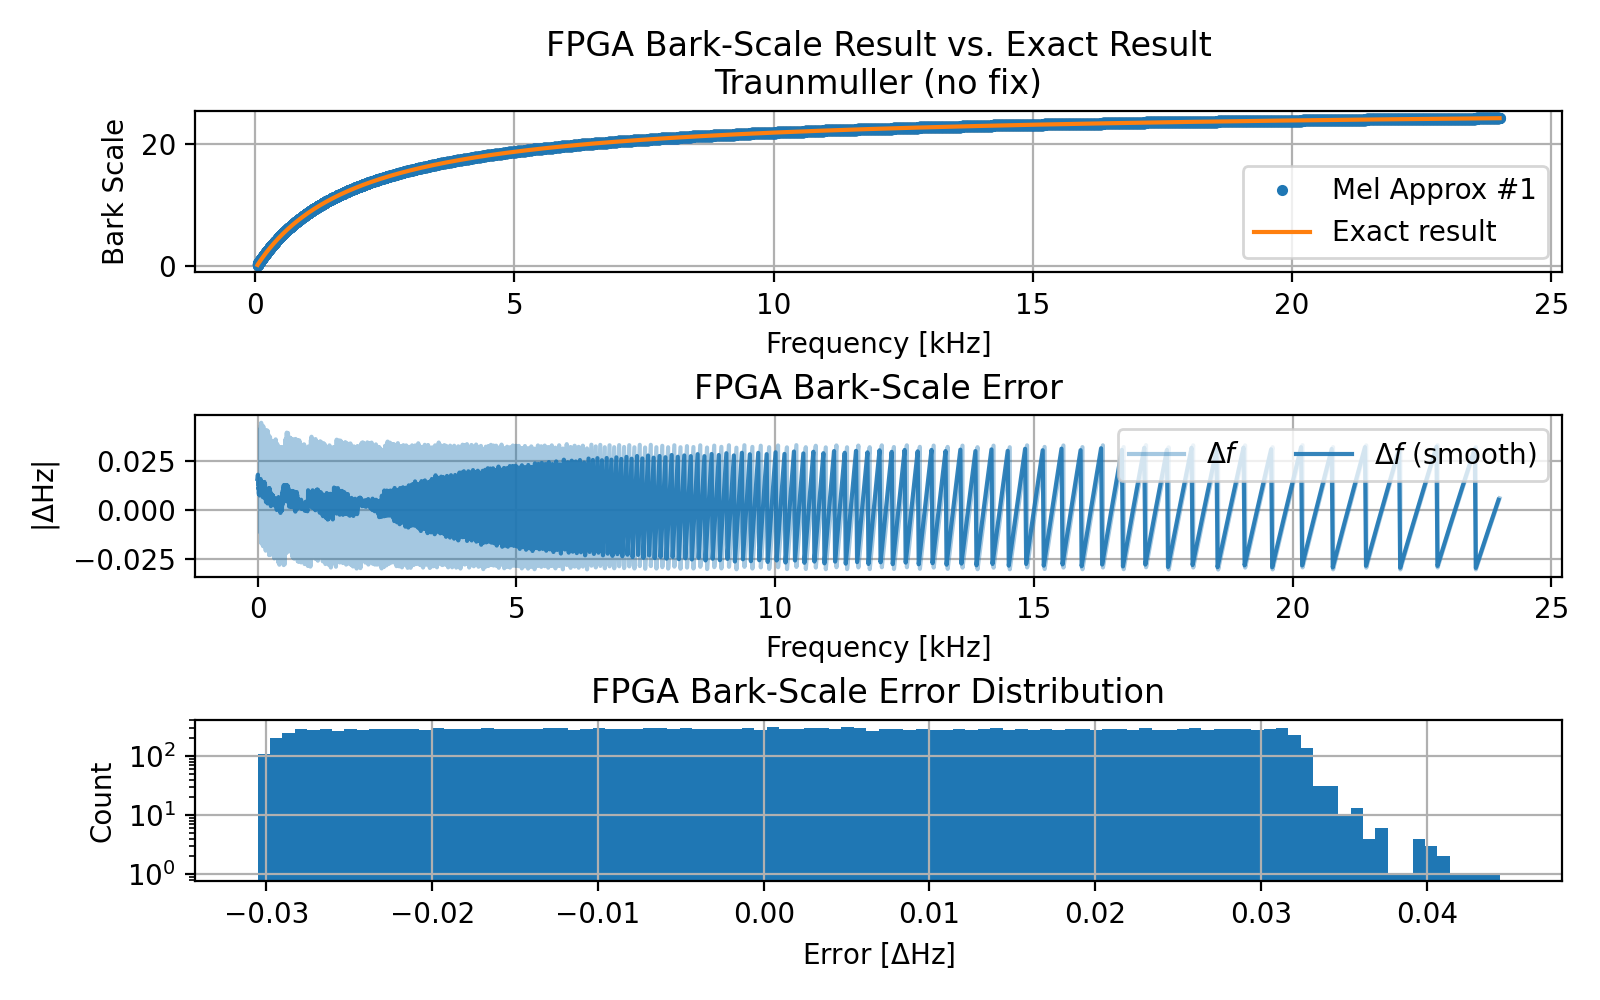
\includegraphics[width=0.75\linewidth]{Scaling/images/bark_traunmuller_no_fix}
    \caption{Schroeder}\label{fig:bark_traunmuller_no_fix}
\end{figure}

\begin{table}[H]
    % for more info see: https://www.overleaf.com/learn/latex/tables
    % \centering
    \hspace*{-1.8cm}
    \arrayrulecolor{mtblborder}
\begin{tabular}{ !{\color{mtblborder}\vrule}l!{\color{mtblborder}\vrule}rcccc| } 
    \hline

    \hline
    \rowcolor{mtblcaption} \color{white}\bf{Algorithm} 
    & \color{white}\bf{Latency \([ns]\)}  
    & \color{white}\bf{Quant.} 
    & \color{white}\bf{Max Err. \([\Delta Hz]\)}
    & \color{white}\bf{Mean Err.}
    & \color{white}\bf{Std Err.} \\
    \hline

    \hline
    \rowcolor{mtbl} Traunmuller w/ Fix   & 14 (3 C.C) & U10/5 & N.A & N.A & N.a \\
    \hline
    
    \hline
    \rowcolor{wtbl} Traunmuller w/o Fix  & 9 (2 C.C) &  U9/4  & 0.0443 & 0.0015 & 0.0180 \\
    \hline

    \hline
\end{tabular}
\arrayrulecolor{black}
\caption{Traunmuller's Bark scale implementations performance comparison}
\label{tbl:bark_implementations_performance}
\end{table}


\begin{table}[H]
    % for more info see: https://www.overleaf.com/learn/latex/tables
    \centering
    \arrayrulecolor{ytblborder}
\begin{tabular}{ !{\color{ytblborder}\vrule}l!{\color{ytblborder}\vrule}rrrrr| } 
    \hline

    \hline
    \rowcolor{ytblcaption} \color{white}\bf{Algorithm} 
    & \color{white}\bf{FF} 
    & \color{white}\bf{LUT} 
    & \color{white}\bf{DSP} 
    & \color{white}\bf{LUTRAM} 
    & \color{white}\bf{BRAM} \\
    % & \color{white}\bf{ORM} 
    % & \color{white}\bf{Clean} \\
    \hline

    \hline
    \rowcolor{ytbl} Traunmuller w/ Fix   & 43(0.02\%) & 302(0.26\%) & 1(<1\%) & 0(0\%) & 0(0\%)  \\
    \hline
    
    \hline
    \rowcolor{wtbl} Traunmuller w/o Fix      & 27(0.01\%) & 284(0.24\%) & 1(<1\%) & 0(0\%)  & 0(0\%)    \\
    \hline

    \hline
\end{tabular}
\arrayrulecolor{black}
\caption{Traunmuller's Bark scale implementations resource utilization table}
\label{tbl:Bark_resource_util}
\end{table}


\begin{table}[H]
    % for more info see: https://www.overleaf.com/learn/latex/tables
    \centering
    \arrayrulecolor{gtblborder}
\begin{tabular}{ |l|cc| } 
    \hline

    \hline
    \rowcolor{gtblcaption} \color{white}\bf{Parameter} 
    & \color{white}\bf{Traunmuller w/ Fix} 
    & \color{white}\bf{Traunmuller w/o Fix} \\
    \hline\hline
    \rowcolor{wtbl}\multicolumn{3}{|c|}{\bf{Dynamic Power [W]}}\\
    \hline
    \rowcolor{gtbl} Signals                 & 2.380 & 2.192   \\
    \hline
    
    \hline
    \rowcolor{wtbl} Logic                   & 3.079 & 2.957   \\
    \hline

    \hline
    \rowcolor{gtbl} DSP                     & 1.445 & 0.014  \\
    \hline
    
    \hline
    \rowcolor{wtbl} I/O                     & 4.022 & 4.022  \\
    \hline
    
    \hline
    \rowcolor{gtbl} \(\mathbf{P_{dynmic}}\) & \textbf{10.923} & \textbf{\color{gtblborder}9.186}  \\
    \hline

    % \hline
    % \rowcolor{gtbl} Bark Scale      & 56(0.02\%) & 218(\%) & 1(<1\%)   \\
    % % \cline{2-8}
    % % \multirow{-2}{*}{\cellcolor{ytbl}\#1(5)}   & 14.03/17.78 & 27.06 & 13.73 & - & - & - & 7.72 \\ 
    \hline\hline
    \rowcolor{wtbl}\multicolumn{3}{|c|}{\bf{Static Power [W]}}   \\
    \hline

    \hline
    \rowcolor{gtbl} PL Static               & 0.469 & 0.437  \\
    \hline
    
    \hline
    \rowcolor{wtbl} PS Static               & 0.017 & 0.016   \\
    \hline

    \hline
    \rowcolor{gtbl} \(\mathbf{P_{static}}\) & \textbf{0.486} & \textbf{\color{gtblborder}0.453}   \\
    \hline

    \hline\hline
    \rowcolor{wtbl}\multicolumn{3}{|c|}{\bf{Total Power [W]}}   \\
    \hline

    \hline
    \rowcolor{gtbl} \(\mathbf{P_{total}}\)  & \textbf{11.412} & \textbf{\color{gtblborder}9.639}  \\
    \hline
\end{tabular}
\arrayrulecolor{black}
\caption{Traunmuller's Bark scale implementations Power consumption}
\label{tbl:bark_scale_pwr_tbl}
\end{table}


\section{ERB - Equivalent Rectangular Bandwidth}
Like the Bark scaling method, the ERB scale aims 
to rescale the audio spectrum in different 
bandwidths corresponding to the human hearing ``filters''.

This approach slightly differs from the Bark scale
because the filters' model is according
to a rectangular filter with an equivalent
bandwidth.

\begin{align}\label{eq:erb_eq}
    ERBs = 11.17\ln (47.065 - \frac{676170.42}{f + 14678.5})    
\end{align}

A proposed approximation is given by:
\begin{align}\label{eq:erb_approx_eq}
    ERBs = 21.4 \cdot \log_{10} (1 + 0.00437f)    
\end{align}


% \subsection{ERB Critical Bands}

\begin{figure}[H]
    \centering
    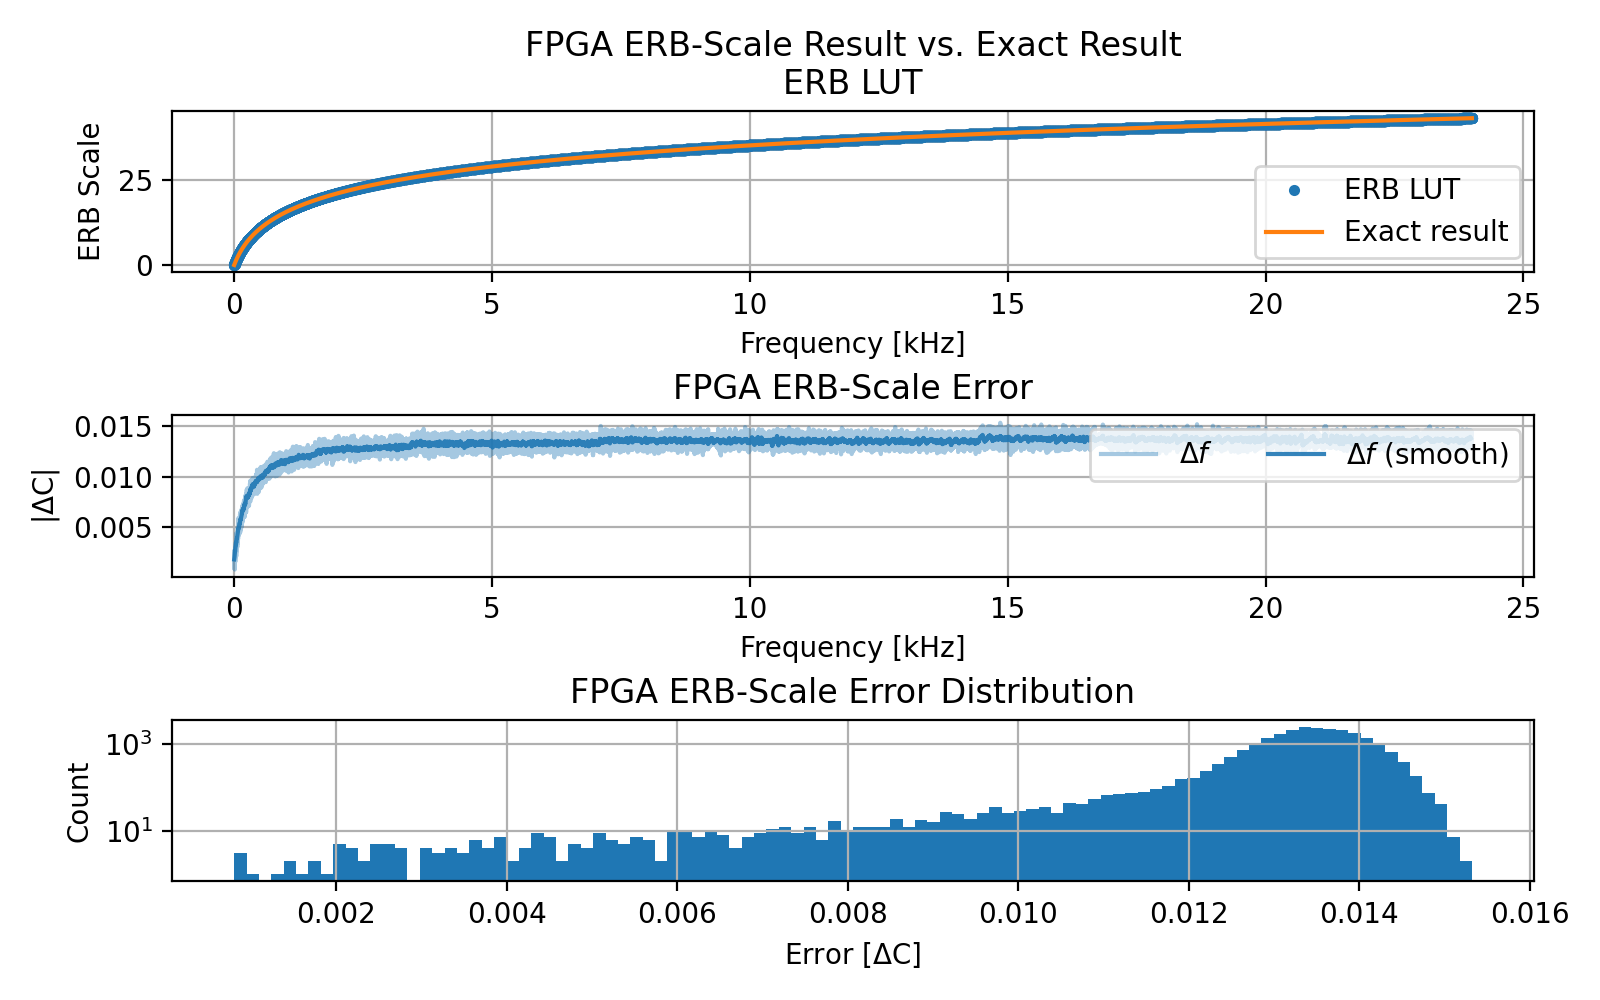
\includegraphics[width=0.75\linewidth]{Scaling/images/erb}
    \caption{LUT based ERB FPGA implementation results}\label{fig:erb_fpga}
\end{figure}


\begin{figure}[H]
    \centering
    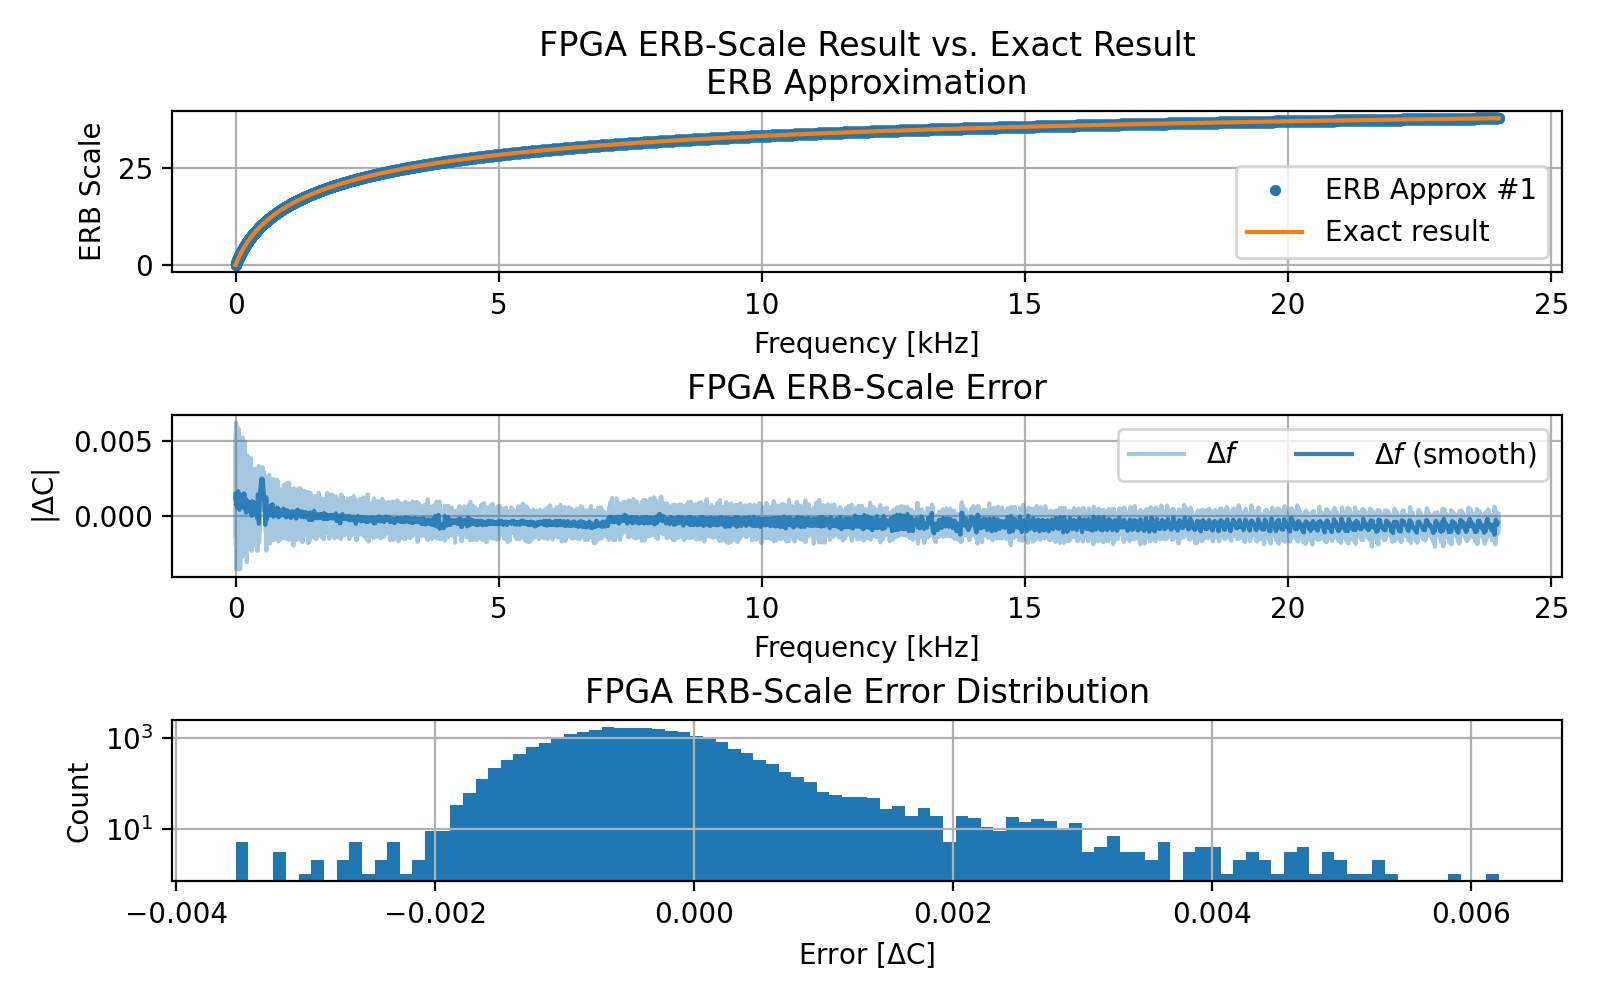
\includegraphics[width=0.75\linewidth]{Scaling/images/erb_approx}
    \caption{LUT based ERB approx. FPGA implementation results}\label{fig:erb_approx}
\end{figure}


\begin{table}[H]
    % for more info see: https://www.overleaf.com/learn/latex/tables
    \centering
    % \hspace*{-1.8cm}
    \arrayrulecolor{mtblborder}
\begin{tabular}{ !{\color{mtblborder}\vrule}l!{\color{mtblborder}\vrule}rcccc| } 
    \hline

    \hline
    \rowcolor{mtblcaption} \color{white}\bf{Algorithm} 
    & \color{white}\bf{Latency \([ns]\)}  
    & \color{white}\bf{Quant.} 
    & \color{white}\bf{Max Err. \([\Delta C]\)}
    & \color{white}\bf{Mean Err.}
    & \color{white}\bf{Std Err.} \\
    \hline

    \hline
    \rowcolor{mtbl} ERB   & 23 (5 C.C) & U16/10 & 0.0153 & 0.0130 & 0.0018 \\
    \hline
    
    \hline
    \rowcolor{wtbl} ERB Approx  & 14 (3 C.C) &  U16/10  & 6.210m & -0.408m & 0.657m \\
    \hline

    \hline
\end{tabular}
\arrayrulecolor{black}
\caption{ERB and ERB approx performance comparison}
\label{tbl:erb_scale_performance}
\end{table}

Table\;\ref{tbl:erb_scale_performance} presents the performance
comparison between the implementations of the pure ERB
and the ERB approximation
given by Equations\;\ref{eq:erb_eq} 
and \ref{eq:erb_approx_eq}, respectively. The error terms
for the ERBs are measured in \(\Delta C\), indicating the
error in Cams rather than in frequency units (Hz). 
Equation\;\ref{eq:cams_hz} can be used to convert Cams to Hz.

\begin{align}\label{eq:cams_hz}
    f = \frac{676170.42}{47.065 - e^{0.0895\cdot C}} - 14678.5
\end{align}

\begin{table}[H]
    % for more info see: https://www.overleaf.com/learn/latex/tables
    \centering
    \arrayrulecolor{ytblborder}
\begin{tabular}{ !{\color{ytblborder}\vrule}l!{\color{ytblborder}\vrule}rrrrr| } 
    \hline

    \hline
    \rowcolor{ytblcaption} \color{white}\bf{Algorithm} 
    & \color{white}\bf{FF} 
    & \color{white}\bf{LUT} 
    & \color{white}\bf{DSP} 
    & \color{white}\bf{LUTRAM} 
    & \color{white}\bf{BRAM} \\
    % & \color{white}\bf{ORM} 
    % & \color{white}\bf{Clean} \\
    \hline

    \hline
    \rowcolor{ytbl} ERB   & 112(0.05\%) & 824(0.70\%) & 1(<1\%) & 1(0.02\%) & 1.5(1.04\%)  \\
    \hline
    
    \hline
    \rowcolor{wtbl} ERB Approx      & 103(0.04\%) & 564(0.48\%) & 1(<1\%) & 1(0.01\%)  & 1.5(1.04\%)    \\
    \hline

    \hline
\end{tabular}
\arrayrulecolor{black}
\caption{Mel scaling methods resource utilization table}
\label{tbl:ERB_resource_util}
\end{table}


\begin{table}[H]
    % for more info see: https://www.overleaf.com/learn/latex/tables
    \centering
    \arrayrulecolor{gtblborder}
\begin{tabular}{ |l|cc| } 
    \hline

    \hline
    \rowcolor{gtblcaption} \color{white}\bf{Parameter} 
    & \color{white}\bf{ERB} 
    & \color{white}\bf{ERB Approx} \\
    \hline\hline
    \rowcolor{wtbl}\multicolumn{3}{|c|}{\bf{Dynamic Power [W]}}\\
    \hline
    \rowcolor{gtbl} Signals                 & 12.691 & 5.525   \\
    \hline
    
    \hline
    \rowcolor{wtbl} Logic                   & 17.576 & 7.478   \\
    \hline

    \hline
    \rowcolor{gtbl} DSP                     & 0.067 & 0.049  \\
    \hline
    
    \hline
    \rowcolor{wtbl} I/O                     & 17.379 & 17.373  \\
    \hline
    
    \hline
    \rowcolor{gtbl} \(\mathbf{P_{dynmic}}\) & \textbf{47.713} & \textbf{\color{gtblborder}31.519}  \\
    \hline

    % \hline
    % \rowcolor{gtbl} Bark Scale      & 56(0.02\%) & 218(\%) & 1(<1\%)   \\
    % % \cline{2-8}
    % % \multirow{-2}{*}{\cellcolor{ytbl}\#1(5)}   & 14.03/17.78 & 27.06 & 13.73 & - & - & - & 7.72 \\ 
    \hline\hline
    \rowcolor{wtbl}\multicolumn{3}{|c|}{\bf{Static Power [W]}}   \\
    \hline

    \hline
    \rowcolor{gtbl} PL Static               & 2.971 & 1.510  \\
    \hline
    
    \hline
    \rowcolor{wtbl} PS Static               & 0.084 & 0.046   \\
    \hline

    \hline
    \rowcolor{gtbl} \(\mathbf{P_{static}}\) & \textbf{3.055} & \textbf{\color{gtblborder}1.556}   \\
    \hline

    \hline\hline
    \rowcolor{wtbl}\multicolumn{3}{|c|}{\bf{Total Power [W]}}   \\
    \hline

    \hline
    \rowcolor{gtbl} \(\mathbf{P_{total}}\)  & \textbf{50.768} & \textbf{\color{gtblborder}33.075}  \\
    \hline
\end{tabular}
\arrayrulecolor{black}
\caption{ERB vs. ERB approx Power consumption}
\label{tbl:erb_scale_pwr_tbl}
\end{table}




% \begin{table}[H]
%     % for more info see: https://www.overleaf.com/learn/latex/tables
%     \centering
%     \begin{tabular}{|c|r|r|r|r|r|}
%       \hline
%       $N$ & Latency ($\mu s$) & FF & LUT & DSP48 & BRAM \\
%       \hline
%         3  & 4.80  &   3889 (27.6\%)                 &    3901 (54.9\%)                  &   90 (25.0\%) & 0 (0.0\%) \\
%         4  & 6.34  &  63657 (45.1\%)                 &   64149 (90.4\%)                  &  144 (40.0\%) & 0 (0.0\%) \\
%         8  & 12.50 & 231199 (\textcolor{red}{164\%}) &  252446 (\textcolor{red}{356\%})  &  272 (75.6\%) & 0 (0.0\%) \\
%         16 & 24.82 & 895377 (\textcolor{red}{635\%}) & 1040992 (\textcolor{red}{1466\%}) &  144 (40.0\%) & 0 (0.0\%) \\
%        \hline
%     \end{tabular}
%     \caption{\bf{ IQRD Performance:} Latency, Resource Utilization, and Power for \(log_{10}\) LUT on FPGA}
%     \label{tbl:IQRD_perf}
% \end{table}

\section{Summary}


\begin{table}[H]
    % for more info see: https://www.overleaf.com/learn/latex/tables
    \centering
    \arrayrulecolor{ytblborder}
\begin{tabular}{ !{\color{ytblborder}\vrule}l!{\color{ytblborder}\vrule}rrrrr| } 
    \hline

    \hline
    \rowcolor{ytblcaption} \color{white}\bf{Algorithm} 
    & \color{white}\bf{FF} 
    & \color{white}\bf{LUT} 
    & \color{white}\bf{DSP} 
    & \color{white}\bf{LUTRAM} 
    & \color{white}\bf{BRAM} \\
    % & \color{white}\bf{ORM} 
    % & \color{white}\bf{Clean} \\
    \hline

    \hline
    \rowcolor{ytbl} Log-Based Mel   & 82(0.04\%) & 276(0.23\%) & 1(<1\%) & 10(0.02\%) & 1.5(1.04\%) \\
    \hline
    
    \hline
    \rowcolor{wtbl} Mel \#1 Generic     & 47(0.02\%) & 269(0.19\%) & 1(<1\%) & 0(0\%)  & 0(0\%)    \\
    \hline
    
    \hline
    \rowcolor{ytbl} Bark Scale w/ fix     & 43(0.02\%) & 302(0.26\%) & 1(<1\%) & 0(0\%) & 0(0\%)  \\
    \hline

    \hline
    \rowcolor{wtbl} Bark Scale w/o fix     & 27(0.01\%) & 284(0.24\%) & 1(<1\%) & 0(0\%)  & 0(0\%)    \\
    \hline

    \hline
    \rowcolor{ytbl} Approx. ERB     & 103(0.04\%) & 564(0.48\%) & 1(<1\%) & 1(0.01\%)  & 1.5(1.04\%)    \\
    \hline

    \hline
\end{tabular}
\arrayrulecolor{black}
\caption{Mel-Approx, log-based Mel, Bark Scale}
\label{tbl:IQRD_perf}
\end{table}



\begin{table}[H]
    % for more info see: https://www.overleaf.com/learn/latex/tables
    % \centering
    \hspace*{-1cm}
    \arrayrulecolor{gtblborder}
\begin{tabular}{ |l|ccccc| } 
    \hline

    \hline
    \rowcolor{gtblcaption} \color{white}\bf{Parameter} 
    & \color{white}\bf{Mel LUT}
    & \color{white}\bf{Mel Gen}
    & \color{white}\bf{Bark w/}
    & \color{white}\bf{Bark w/o}
    & \color{white}\bf{Approx. ERB} \\
    \hline\hline
    \rowcolor{wtbl}\multicolumn{6}{|c|}{\bf{Dynamic Power [W]}}\\
    \hline
    \rowcolor{gtbl} Signals & 4.947 & 2.916 & 2.380 & 2.192 & 5.525  \\
    \hline
    
    \hline
    \rowcolor{wtbl} Logic & 6.50 & 3.070 & 3.079 & 2.957 & 7.478  \\
    \hline

    \hline
    \rowcolor{gtbl} DSP & 0.014 & 0.014 & 1.445 & 0.014 & 0.049  \\
    \hline
    
    \hline
    \rowcolor{wtbl} I/O & 18.236 & 6.378 & 4.022 & 4.022 & 17.373  \\
    \hline
    
    \hline
    \rowcolor{gtbl} \(\mathbf{P_{dynmic}}\) & \textbf{29.697} & \textbf{12.379} & \textbf{10.923} & \textbf{9.186} & \textbf{31.519}  \\
    \hline

    % \hline
    % \rowcolor{gtbl} Bark Scale      & 56(0.02\%) & 218(\%) & 1(<1\%)   \\
    % % \cline{2-8}
    % % \multirow{-2}{*}{\cellcolor{ytbl}\#1(5)}   & 14.03/17.78 & 27.06 & 13.73 & - & - & - & 7.72 \\ 
    \hline\hline
    \rowcolor{wtbl}\multicolumn{6}{|c|}{\bf{Static Power [W]}}   \\
    \hline

    \hline
    \rowcolor{gtbl} PL Static               & 2.364 & 0.499 & 0.469 & 0.437 & 1.510  \\
    \hline
    
    \hline
    \rowcolor{wtbl} PS Static               & 0.068 & 0.018 & 0.017 & 0.016 & 0.046  \\
    \hline

    \hline
    \rowcolor{gtbl} \(\mathbf{P_{static}}\) & \textbf{2.432} & \textbf{0.517} & \textbf{0.486} & \textbf{0.453} & \textbf{1.556}  \\
    \hline

    \hline\hline
    \rowcolor{wtbl}\multicolumn{6}{|c|}{\bf{Total Power [W]}}   \\
    \hline

    \hline
    \rowcolor{gtbl} \(\mathbf{P_{total}}\)  & \textbf{32.13} & \textbf{12.896} & \textbf{11.412} & \textbf{9.639} & \textbf{33.075}  \\
    \hline
\end{tabular}
\arrayrulecolor{black}
\caption{Mel-Approx, log-based Mel, Bark Scale Power consumption}
\label{tbl:sum_scale_pwr_tbl}
\end{table}




% \begin{table}[H]
%     % for more info see: https://www.overleaf.com/learn/latex/tables
%     \centering
%     \arrayrulecolor{gtblborder}
% \begin{tabular}{ !{\color{gtblborder}\vrule}l!{\color{gtblborder}\vrule}rrrrrr| } 
%     \hline

%     \hline
%     \rowcolor{gtblcaption} \color{white}\bf{Algorithm} 
%     & \color{white}\bf{Signals} 
%     & \color{white}\bf{Logic} 
%     & \color{white}\bf{DSP} 
%     & \color{white}\bf{IO} 
%     & \color{white}\bf{BRAM}
%     & \color{white}\bf{Total} \\
%     \hline

%     \hline
%     \rowcolor{gtbl} Log Based Mel   & 82(0.04\%) & 276(\%) & 1(<1\%) & 18 & 1.5 & 0 \\
%     \hline
    
%     \hline
%     \rowcolor{wtbl} Approx. Mel     & 47(0.02\%) & 230(\%) & 1(<1\%) & 0  & 0   & 0 \\
%     \hline
    
%     \hline
%     \rowcolor{gtbl} Bark Scale      & 56(0.02\%) & 218(\%) & 1(<1\%) & 0  & 0   & 0 \\
%     % \cline{2-8}
%     % \multirow{-2}{*}{\cellcolor{ytbl}\#1(5)}   & 14.03/17.78 & 27.06 & 13.73 & - & - & - & 7.72 \\ 
%     \hline

%     \hline
% \end{tabular}
% \arrayrulecolor{black}
% \caption{Mel-Approx, log based Mel, Bark Scale Power consumption}
% \label{tbl:scale_pwr_tbl}
% \end{table}


\begin{table}[H]
    % for more info see: https://www.overleaf.com/learn/latex/tables
    % \centering
    \hspace*{-1.8cm}
    \arrayrulecolor{mtblborder}
\begin{tabular}{ !{\color{mtblborder}\vrule}l!{\color{mtblborder}\vrule}rcccc| } 
    \hline

    \hline
    \rowcolor{mtblcaption} \color{white}\bf{Algorithm} 
    & \color{white}\bf{Latency \([ns]\)}  
    & \color{white}\bf{Quant.} 
    & \color{white}\bf{Max Err. \([\Delta Hz]\)}
    & \color{white}\bf{Mean Err.}
    & \color{white}\bf{Std Err.} \\
    \hline

    \hline
    \rowcolor{mtbl} Log-Based Mel   & 14 (3 C.C) & U16/4 & 1.146 & 0.268 & 0.106 \\
    \hline
    
    \hline
    \rowcolor{wtbl} Mel \#1 Generic     & 9 (2 C.C) &  U16/4  & 0.174 & -0.035 & 0.061 \\
    \hline
    
    \hline
    \rowcolor{mtbl} Bark Scale w/ fix      & 14 (3 C.C) &  U10/5 & N.A & N.A & N.A \\
    % \cline{2-8}
    % \multirow{-2}{*}{\cellcolor{ytbl}\#1(5)}   & 14.03/17.78 & 27.06 & 13.73 & - & - & - & 7.72 \\ 
    \hline

    \hline
    \rowcolor{wtbl} Bark Scale w/o fix     & 9 (2 C.C) &  U9/4  & 0.0443 & 1.5m & 0.0015 \\
    \hline

    \hline
    \rowcolor{mtbl} ERB Approx.     & 14 (3 C.C) &  U16/10  & 0.292 & 0.104 & 0.134 \\
    \hline

    \hline
\end{tabular}
\arrayrulecolor{black}
\caption{Mel-Approx, log-based Mel, Bark Scale performance comparison}
\label{tbl:scale_pwr_tbl}
\end{table}




  \cleardoublepage
  \printbibliography[title={References}]
\end{refsection}

\begin{refsection}[Features/features.bib]
  
% Take from PyAudioAnalysis
% short-term, mid-term features

% \chapter{Algorithms}
% \section{Time Analysis}
% \subsection{Convolution}
% A general use of the convolution operation
% is to evaluate the outputs of linear
% time-invariant systems.
% Taking the impulse response of a system, and
% applying the convolution with
% a given input, gives the system's output
% for that specific input.

% For continuous time dependent arguments,
% \(x\) as the input variable, and \(h\) as the
% system's impulse response, the convolution is given by:

% \begin{equation}
%     (x * h)(t) \triangleq \int^{\infty}_{-\infty} x(t)h(t-\tau) d\tau
% \end{equation}

% Due to the commutativity property of the convolution
% operation, the shifting over one of the arguments
% is interchangeable, thus one can write
% the same equation as:

% \begin{equation}
%     (x * h)(t) \triangleq \int^{\infty}_{-\infty} x(t-\tau)h(t) d\tau
% \end{equation}

% Likewise, working with discrete variables,
% the convolution operation can be written as:
% \begin{align}
%     (x * h)[n] \triangleq & \sum^{\infty}_{m=-\infty} x[m]h[n-m] \\
%     (x * h)[n] \triangleq & \sum^{\infty}_{m=-\infty} x[n-m]h[m]
% \end{align}


% \subsection{Cross-Correlation}
% Cross-correlation is an operation that can measure
% how similar two functions are. By ``shifting''
% one function over the other and measuring the amount
% of correlation at each given point, the output graph
% demonstrates at what ``distance''
% the maximum similarity occurs,
% in correspondence
% to the graph's maximum amplitude.

% \begin{align}
%     (x * h)(t) \triangleq & \int^{\infty}_{-\infty} x^{*}(t)h(t+\tau) d\tau \\
%     (x * h)(t) \triangleq & \int^{\infty}_{-\infty} x^{*}(t-\tau)h(t) d\tau
% \end{align}

% \begin{align}
%     (x * h)[n] \triangleq & \sum^{\infty}_{m=-\infty} x^{*}[m]h[n+m] \\
%     (x * h)[n] \triangleq & \sum^{\infty}_{m=-\infty} x^{*}[n-m]h[m]
% \end{align}

% \subsection{Auto-Correlation}
% In a case where the two input functions
% of the cross-correlation are the same input signals,
% the measure is then called ``auto-correlation''.
% In other words, this measure demonstrates
% at what ``distance'' the delayed version of the signal
% most matches the original version of it.

% This kind of measure is very useful in audio
% applications where multi-microphones are spread
% with varying distance from each other and from the
% source. Looking for the maxima point of the
% auto-correlation between the signal received by
% the microphones, one can deduce the lag time
% that best characterizes the microphones' formation.

% Several enhancement and manipulation techniques
% are then become available when the lagging
% time is known.
% For example the delay and sum algorithm beamforming
% algorithm for constructive summation of the different
% channels that translates
% to better SNR (signal-to-noise ratio).

% \subsubsection{Covariance Matrices}
% \begin{equation}
%     \mathbf{R}_{XY} \triangleq \mathbf{E}[XY^{tr}]
% \end{equation}

% \begin{align}
%     \mathbf{R}_{XX} & \triangleq \mathbf{E}[XX^{tr}] \\
%                     & = \frac{1}{T} \sum^{T-1}_{t=0}
%     {X}(t;j\omega){X}^{\mathbf{H}}(t;j\omega)
% \end{align}

% Where the \(\mathbb{H}\) operator
% is the \emph{Hermitian function} which stands for
% the complex conjugate.

% % ESPNet \& Mirco Document
% \subsection{Sinc-Conv}

% % \begin{figure}[ht]
% %     \centering
% %     \includegraphics[width=0.99\textwidth]
% %     {./img/Comparison_convolution_correlation.svg}\label{fig:conv_vs_corr_plot}
% %     \caption{Convolution vs. Cross-Correlation vs. Auto-Correlation plot [Wikipedia]}
% % \end{figure}



% \section{Frequency Analysis}
% \subsection{DTFT}
% \begin{equation}
%     X_{2\pi}(\omega) = \sum_{n=-\infty}^{\infty} x[n] \,e^{-i \omega n}
% \end{equation}


% \subsection{IDTFT}
% \begin{equation}
%     x[n] = \frac{1}{2 \pi}\int_{2\pi} X_{2\pi}(\omega)\cdot e^{i \omega n} d\omega
% \end{equation}

% \subsection{DFT}
% \begin{equation}
%     \label{eq:dft}
%     X_k = \sum_{n=0}^{N-1} x_n \cdot e^{-\frac {i 2\pi}{N}kn}
% \end{equation}

% Taking Euler's identity:
% \begin{equation}
%     e^{ix} = \cos x + j\sin x
% \end{equation}

% Substituting the exponent power in Equation\;\ref{eq:dft} with the Euler identity
% gives:
% \begin{equation}
%     X_k = \sum_{n=0}^{N-1} x_n \cdot \left[\cos\left(\frac{2 \pi}{N}kn\right)
%         - i \cdot \sin\left(\frac{2 \pi}{N}kn\right)\right]
% \end{equation}


% \subsection{IDFT}
% \begin{equation}
%     x[n] = \frac{1}{N} \sum_{k=0}^{N-1} X_k\cdot e^{i \frac{2 \pi}{N} k n}
% \end{equation}


% \subsection{FFT --- Fast Fourier Transform}

% \subsection{Discrete Cosine Transform (DCT)}

% \begin{equation}
%     y[n] = \sum^{}_{}
% \end{equation}

% \section{Time-Frequency Analysis}
% \subsection{STFT - Short Time Fourier Transfer}

% \subsection{Spectrogram}

% \section{Windows}
% \subsection{Overview}


% \subsection{Rect (boxcar)}
% \subsection{Triangle}
% \subsection{Bartlett}
% \subsection{Hamming}
% \subsection{Hann}
% \begin{align}
%     w[n] = 0.5 - 0.5\cos\left( \frac{ 2\pi n }{ M - 1 } \right) & \qquad 0 \leq n \leq M-1
% \end{align}


% % \subsection{Kaiser}
% % \subsection{Analog Filters}

% \subsection{Overlap + Add Reconstruction}
% % \subsection{Wavelets}

% \section{Speech-Enhancement}
% See table
% \begin{figure}[ht]
%     \centering
%     \includegraphics[width=0.99\textwidth]
%     {./img/spc_enhance_tbl}\label{fig:asr_blocks_diagram}
%     \caption{General E2E ASR System Blocks Diagram}
% \end{figure}



% DCT + MFCC Connection
% DST - Discrete Sine Transforms
% Hilbert Transform
% Analytical Signal
% Wavelates
% Convolution / Correlation
% Parseval's Theorm
% PSD
% Median Filter
% ORder Filter
% Wiener Filter
% Hermitian FFTs





\chapter{Features}\label{ch:features}
\section{Introduction}
In data analysis craftsmanship, 
prominence importance exists 
about how to characterize the data so that 
variations in data characteristics would 
be noticeable and more 
easily discernible during the analysis process.
To that end, the input data being analyzed is reorganized
according to selected features on which
conclusions and distinctive deductions can be made.

Similarly, in a supervised learning 
procedure of a machine, 
in order to make classification decisions accurately. 
The need for such features arises to 
aid the learning algorithm in focusing on the 
same features that probably were selected manually.
An intelligent choice of the learnable features 
\cite{7845025} 
can drastically change a given model's outcomes quality.
In a supervised learning, the 
feature selection and extraction process withal,
are preparatory steps to the learning or classification
stages coming next.
As a rule of thumb, the more features, the better accuracy
a learning model can yield theoretically\cite{lessIsMore}.
That saying holds true to a great degree
as long as often sudden fluctuations do not characterize the data.
In a case of heavy fluctuating characterizations of the data,
or alternatively, in the case of a 
massive number of features, 
that some of which have minor contributions 
to the classification part of the output,
increase in the number of features may become deteriorative.
In terms of performance, 
enlarging the number of features leads to a bigger model, 
an increased number of learnable parameters, 
longer training times, 
and unnecessary extension of processing times.
Also, a possible reduction in the accuracy is 
expected due to 
False-Negative (FN) or False-Positive (FP) 
misdetections resulting from the wrong 
classification of signals as noise and 
vice versa caused by additional redundant features.

For speech signals, a wide variety of 
meaningful feature sets exist. 
More or less useful, different speech features 
may better fit certain use-cases or fulfill 
a particular unerring task. 
Features for speech (including audio) 
are mainly from the following domains:
\begin{enumerate}
    \item Spectral Features
    \item Cepstral Features
    \item Time domain Features
    \item Spatial Features
\end{enumerate}

Speech features are selected 
to give the maximal accuracy in detecting utterances.
That means a precise characterization of a 
word, utterance, or the pronunciation of 
a single character, making them distinguishable
from other input streams. 

\section{Spectral Features}
\subsection{FB --- FilterBanks}
FilterBanks is a very common technique
for spectral mapping of speech signals.
By dividing the audio spectrum into multiple 
sub-domains with a defined level of overlap, 
the spectrum is 
``framed'' according to frequency. 
Thus, by a set of band-pass filters,
each frame contains the confined 
information of the speech signal 
that corresponds to the filter's specific 
range of frequencies.

The resolution can then be set as a function of
the number of filters and the overall processed audio bandwidth.
Increasing the number of filters, assuming the 
audio bandwidth and the overlap ratio are constant, means
narrower allocated bandwidths for each individual filter
or in other better spectral resolution.

Filterbanks by themselves are not the desired speech feature,
but only the mean for feature extraction. 
The most common feature extracted by a Filterbank set
is the total sum of energy bounded by the filter's frequency response.
A set of filters is computed per 
frequency bin and remains the same for 
the entire signal length over time.
Thus, the total sum of energy computed for 
each filter characterizes the 
speech over a finite defined duration of time.

The human hearing system is less sensitive to high frequencies
than lower band frequencies, as described in Chapter\;\ref{ch:scaling_methods}.
Therefore, in an attempt to emulate the same natural behavior and
resemble the hearing ``filters'' as much as possible, 
the Filterbank set of filters is set with center frequencies
according to the different scaling 
methods described in Chapter\;\ref{ch:scaling_methods}.
In that way, narrow-band filters are assigned to 
lower frequency ranges. 
Similarly, wide-band filters are for 
the higher hearable frequency ranges.

\subsubsection{Mel FB}
One way of mapping the audio spectrum is according to the Mel
scale. This scaling method is described in Chapter\;\ref{ch:scaling_methods}.
First, the center frequencies and the bandwidths are received by the transformation
between Herz to Mels. Then a set of Bartlett
filters with those center frequencies are generated
with an overlap of 50\% between adjacent filters. 


The amplitude of the filters is bounded to \(1\) 
to maintain NOLA compatibility.
An example of a Mel Filterbank constructed by Bartlett filters
is shown in Figure~\ref{fig:sb_mel_fb}.
\begin{figure}[H]
    \centering
    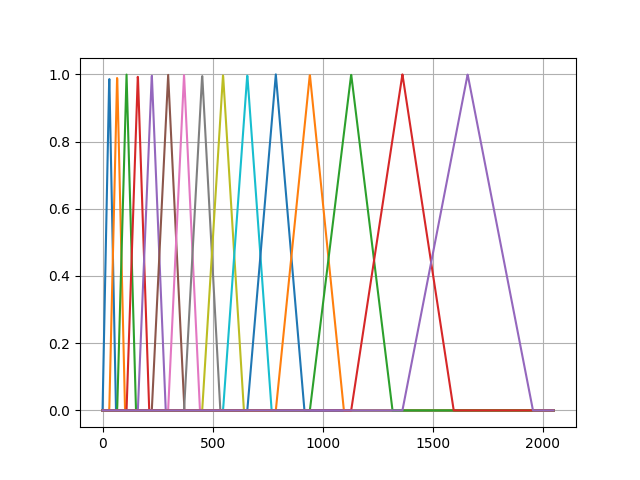
\includegraphics[width=0.75\linewidth]{Features/images/sb_mel_fb}
    \caption{Mel FB}\label{fig:sb_mel_fb}
\end{figure}

\subsubsection{Bark FB}
The Bark Filterbank is very similar to the Mel Filterbank
except that it follows the Bark scale 
instead of the Mel Scale.

Different filter shapes are available but, 
triangular filter shapes are the most common,
as described in \cite{barkfilt}.

An example of the Bark Filterbank constructed by Bartlett filters
is shown in Figure~\ref{fig:mat_bark_fb}.
\begin{figure}[H]
    \centering
    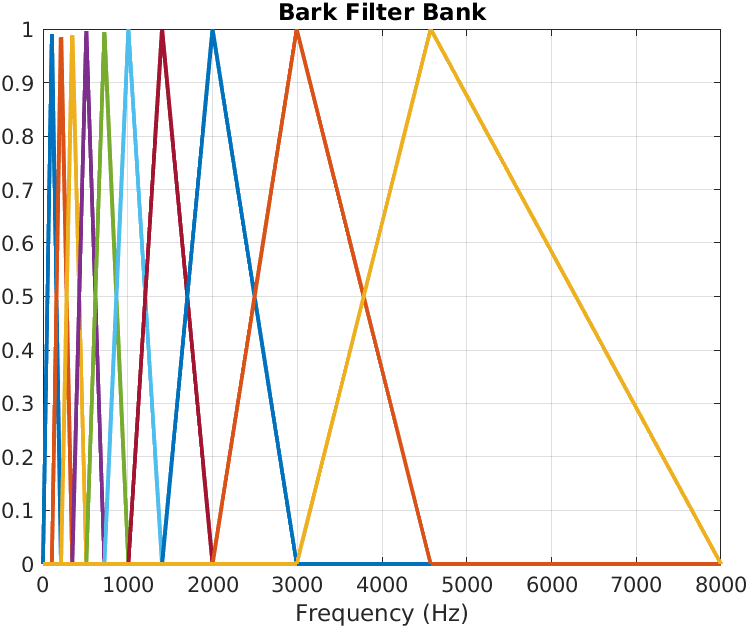
\includegraphics[width=0.75\linewidth]{Features/images/mat_bark_fb}
    \caption{Bark FB}\label{fig:mat_bark_fb}
\end{figure}

\subsubsection{Gammatone FB}
The Gammatone filter, as described in \cite{gammatonefilt},
has a response function as follows:
\begin{equation}
    g(t) = \alpha t^{n-1}e^{-2\pi bt}\cos \left( 2\pi f_{c} t + \phi\right)
\end{equation}

Where \(\alpha\) denotes the amplitude factor,
\(n\) is the filter order,
\(f_{c}\) is the center frequency,
\(\phi\) is the phase factor,
and \(b\) is the bandwidth parameter
computed according 
to the ERB scale mapping of \(1.019\cdot ERB \left( f_{c} \right)\).

An example of a Gammatone Filterbank
is shown in Figure~\ref{fig:sb_fb_gauss}.
\begin{figure}[H]
    \centering
    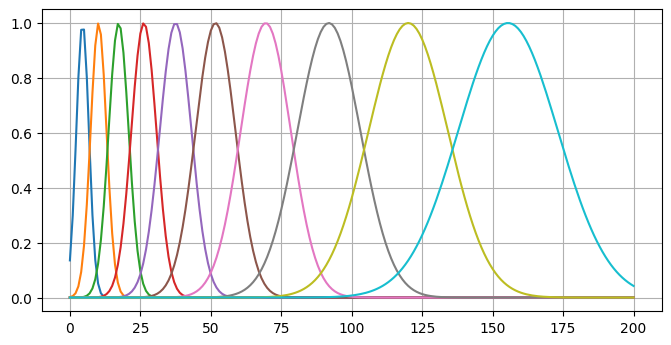
\includegraphics[width=0.75\linewidth]{Features/images/sb_fb_gauss}
    \caption{Gammatone FB}\label{fig:sb_fb_gauss}
\end{figure}


\section{Cepstral Features}
\subsection{MFCCs --- Mel-Frequency Cepstral Coefficients}

% https://link.springer.com/content/pdf/bbm%3A978-3-319-03116-3/1.pdf
\subsubsection{Pre-emphasis}
Speech signals have a roll-off frequency 
resembling a low-pass behavior\cite{237532}.
Due to that physical nature, higher frequencies 
decay faster than lower speech frequencies.
Compensation for this phenomenon is attainable with a 
pre-emphasis filter that boosts 
the higher\cite{7489370} frequencies responses.


\subsubsection{Framing}
Speech signals vary in time. 
Although the variation over time is relatively slow, 
a speech signal is a non-pure stationary process 
but a quasi-stationary. 
Therefore, analysis of speech signals 
is taken on small portions of the 
signal to be less affected by randomness effects.
To that end, a preliminary framing action is applied
to to speech signals in the time domain.
Framing means dividing the signal 
into small fragments(frames) with some overlapping in between.
Each time frame is assumed to be stationary,
and thus a measurement can be taken.

The shifting in time between frames is referred
to as the hopping length and is set to contain 
a sufficient amount of temporal
context that characterizes the natural
characteristics of speech.

A very common sampling frequency of audio signals
is \(16KHz\). 
As a result, and in order to work with 
a round number of sampling points, 
the frame lengths 
and the hopping lengths 
are set to \(25ms\), and 
\(6.25ms\) or \(10ms\) for hopping size. 
These values translate to a frame length
equals 400 sampling points, and hopping size
equals 100 or 160 sampling points, respectively.
Another advantage of setting the hopping length
as \(6.25ms\) is that it gives
a complete temporal context of 3 adjacent frames
by definition.

\subsubsection{Windowing}
In order to extract each frame only 
whilst also minimizing the Gibbs effects as much as possible,
a windowing function is applied.
As a result, the information confined 
in a given frame is extracted while the 
window's response function tapers 
the edges to reduce the adjacent frames' effect.

Usually, a Hamming or a Hann window 
is used as the window function due to their 
relatively decent trade-off between edge tapering, 
implementation simplicity, bandwidth, and spectral leakage, 
making them exceptionally suitable for speech signals.

The Hamming and Hann windows are given by
Equations\;\ref{eq:hammwin} and \ref{eq:hannwin}, respectively.
\begin{align}
    \label{eq:hammwin} &W_{_{Hamming}}[n] = 0.54 - 0.46
    \cos\left( \frac{2\pi n}{M-1} \right) &
            0 \leq n \leq M - 1 \\
    \label{eq:hannwin} &W_{_{Hann}}[n] = 0.5 - 0.5
            \cos\left( \frac{2\pi n}{M-1} \right) &
            0 \leq n \leq M - 1
\end{align}

\subsubsection{DFT spectrum}
Each one of the windowed frames is
converted to the frequency domain by applying the 
Discrete Fourier Transform (DFT).
The composition of both windowed framing 
and the DFT is referred to as the 
Short-Time Fourier Transform (STFT).
A technique to visualize the STFT outcome is 
called a spectrogram. The STFT outcome contains 
multiple frequency bins per time frame,
making it a function of \(f, t\).

The DFT is given by:
\begin{align}
    X_{m}(f) = \sum_{n=-\infty}^{\infty} x[n]g[n-mR]e^{-j2\pi fn}
\end{align}

Where \(X_{m}(f)\) denotes the DFT transformation of
a given time frame windows signal,
\(g[\circ]\) denotes the window function of size \(M\),
and \(R\) represents the hopping size.

\begin{figure}[H]
    \centering
    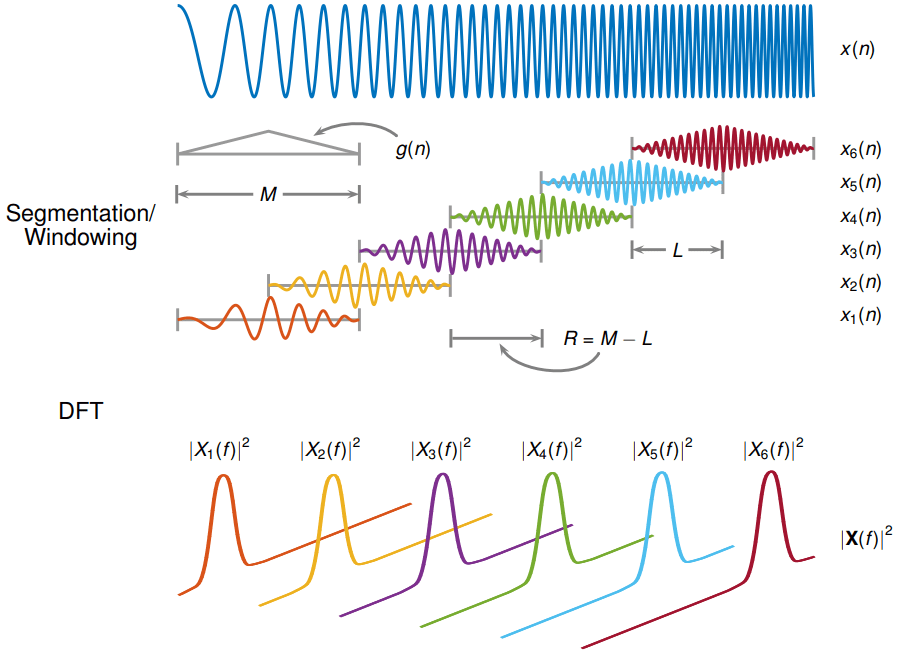
\includegraphics[width=\linewidth]{Features/images/iscola_stft}
    \caption{STFT demonstration diagram}\label{fig:iscola_stft}
    \source{Adapted from Matlab's STFT documentation}
\end{figure}

\subsubsection{Mel-spectrum}
Once the spectrogram is received, 
the frequencies are rescaled in accordance with the Mel Scale.
A comprehensive description of the Mel Scale 
is detailed in Chapter\;\ref{ch:scaling_methods}.

Next, the cepstral coefficients are extracted from each frequency bin, 
by taking the energies sum of each filter and multiplying it
with the Discrete Cosine Transform (DCT).
\begin{align}\label{eq:mfcc}
    MFCC[n] & = \sqrt{\frac{2}{K}} \sum_{k=1}^{K} \left\{ 
        e[k] \cdot DCT\left( k \right)
     \right\} \nonumber \\
     & = \sqrt{\frac{2}{K}} \sum_{k=1}^{K} \left\{ 
        e[k] \cdot \cos \left( \frac{\pi n}{K} (k+0.5) \right)
     \right\}
\end{align}

It is very common to extract the log-Mel energies
and then have Equation\;\ref{eq:mfcc} written as:
\begin{align}\label{eq:logmfcc}
    MFCC[n] & = \sqrt{\frac{2}{K}} \sum_{k=1}^{K} \left\{ 
        \log \left( e[k] \right) \cdot \cos \left( \frac{\pi n}{K} (k+0.5) \right)
     \right\}
\end{align}

% Take from PyAudioAnalysis
% PyAudioProcessing

\subsection{RFCCs --- Root-Frequency Cepstral Coefficients}
An alternative to the log-Mel 
extraction of the cepstral coefficients
has been suggested in \cite{rmfcc1} and \cite{1415167}.
The motivation to put this proposed 
technique under test is that the root 
function can be less computationally demanding 
than the traditional log function..
\begin{align}
    RCC[n] & = \sqrt{\frac{2}{N}} \sum_{k=1}^{K} \left\{ 
        \left( e[k] \right)^{\gamma} \cdot \cos \left( \frac{\pi n}{K} (k+0.5) \right)
     \right\}
\end{align}

\subsection{GFCCs --- Gammatone-Frequency Cepstral Coefficients}
GFCCs follow the basic steps same as the MFCCs extraction.
But, instead of translating the frequencies to Mels,
the spectrum is translated to the ERB scale.
ERB scale implies a Gammatone Filterbank as described in Chapter \ref{ch:scaling_methods}.


\subsection{BFCCs --- Bark-Frequency Cepstral Coefficients}
Like the Gammatone-FCCs (GFCCs), the BFCCs follow the Bark Scale.

% \subsection{LFCCs --- Linear-Frequency Cepstral Coefficients}
% \subsection{LPC --- Linear Predictive Coefficients}
% \subsection{MSRCC --- Magnitude-based Spectral Root Cepstral Coefficients}
% \subsection{NGCC --- Normalized Gammachirp Cepstral Coefficients}
% \subsection{PNCC --- Mel-Frequency Cepstral Coefficients}
% \subsection{PSRCC --- Mel-Frequency Cepstral Coefficients}
% \subsection{RPLP --- Mel-Frequency Cepstral Coefficients}
% https://spafe.readthedocs.io/en/latest/features/_features.html
% \subsection{articulatory cepstral coefficients}

\section{Time-Domain Features}
\subsection{Dynamic FCC features}
During the framing process, the speech signal 
is divided into small fragments of the speech over time. 
These time unit fragments are called frames.
Each frame spans over a finite time duration.
The extracted cepstral coefficients are computed statically
for a given frame. However, the original speech
is framed in multiple numbers of frames. 
Therefore, coefficients extractions
have to be dynamic for the entire signal, i.e., all frames.

Additional information about the temporal 
changes between adjacent coefficients can also be extracted
to include the dynamics and transitions within a frame.

\subsubsection{Deltas}
The first derivate of the cepstral coefficients
,\(\Delta\) (Deltas),
represents the velocity of the MFCCs' dynamics and 
is a sub-set of the cepstral coefficients.

Deltas (\(\Delta\)) are extracted by:
\begin{equation}\label{eq:deltaderiv}
    \Delta [n] = \frac{ \sum\limits_{i=-T}^{T} k_{i} c_{m}[n+i]}
    {\sum\limits_{i=-T}^{T} |i|}
\end{equation}

Where \(n\) denotes the frame time index, \(k\) marks the 
coefficient weight, \(T\) stands for the number of temporally
adjacent frames used for the calculation, and \(c_{m}\) denotes the
\(m\)th coefficient in the given frame \(n\).

\subsubsection{Delta-Deltas}
Delta-Deltas (\(\Delta\Delta\)) is an extra layer of information
representing the acceleration at which the 
MFCCs' dynamics change within a given time frame.
The extraction of the Delta-Deltas follows the same principale
as the first derivatives. Yet, instead of taking the
cepstral coefficients as the input feature, we replace
\(c_{m}\) in Equation\;\ref{eq:deltaderiv} 
with the first-order derivatives \(\Delta[n]\).

\subsection{Temporal Context}
Temporal context is an attachment of raw unprocessed 
features' data from adjacent
frames together with the currently selected feature. 
Whether spectral, cepstral, or spatial features,
the concatenation of past and future 
features can infer decisions based on a memory effect.
Furthermore, different languages
introduce contextual constraints such as relative positions
of adjectives or nouns to verbs, plurals, affiliations,
possessions, and other lingual principles.

Usually, the number of adjacent past and future frames 
to concatenate is based on the framing and DFT parameters.
It is plain to understand 
one would not want to exaggerate and excessively use
redundant frames that do not have any significant impact
on the accuracy of detection. 
The downside of overly using temporal context frames is obvious, 
orders of magnitude larger amounts of information to process.

% \section{Spatial Features}
% \subsection{VTLN - vocal track length norm}

  \cleardoublepage
  \printbibliography[title={References}]
\end{refsection}

\begin{refsection}[Features/time_freq_masking.bib]
  \chapter{Time-Frequency Masking}
\section{Introduction}
Speech separation, in similarity to other 
prevalent enhancement applications, such as the 
Computational Auditory Scene Analysis (CASA)\cite{BROWN1994297}
and Blind Speech Separation (BSS)\cite{6709849},
makes use of various
algorithms in order to distinguish in one way or another
between desired speech and interferences.
The advantages of precise distinction 
between speech and interference include, among others,
the ability to apply speech enhancements, 
noise cancelation or reduction, speech corrections, and more.
With ASR systems, these abilities are expressed in 
improved performance of precisely detecting words
with higher detection rates.

A typical algorithm in CASA applications is the 
Time-Frequency Masking (T-F Masking). 
Since speech signals vary with time, 
as described in chapter \;\ref{ch:features}, 
they are not considered stationary. 
Hence, a unique representation is required 
for conducting an accurate analysis of such signals. 

A T-F representation means presenting a speech 
signal in time-frequency composition, 
where each T-F unit contains the 
speech's spectral elements at a certain time window bin. 
As described in chapter\;\ref{ch:features}, 
the T-F presentation of a signal 
arrives by using the STFT or auditory filtering\cite{Xia2017UsingOR}.

\begin{figure}[H]
    \centering
    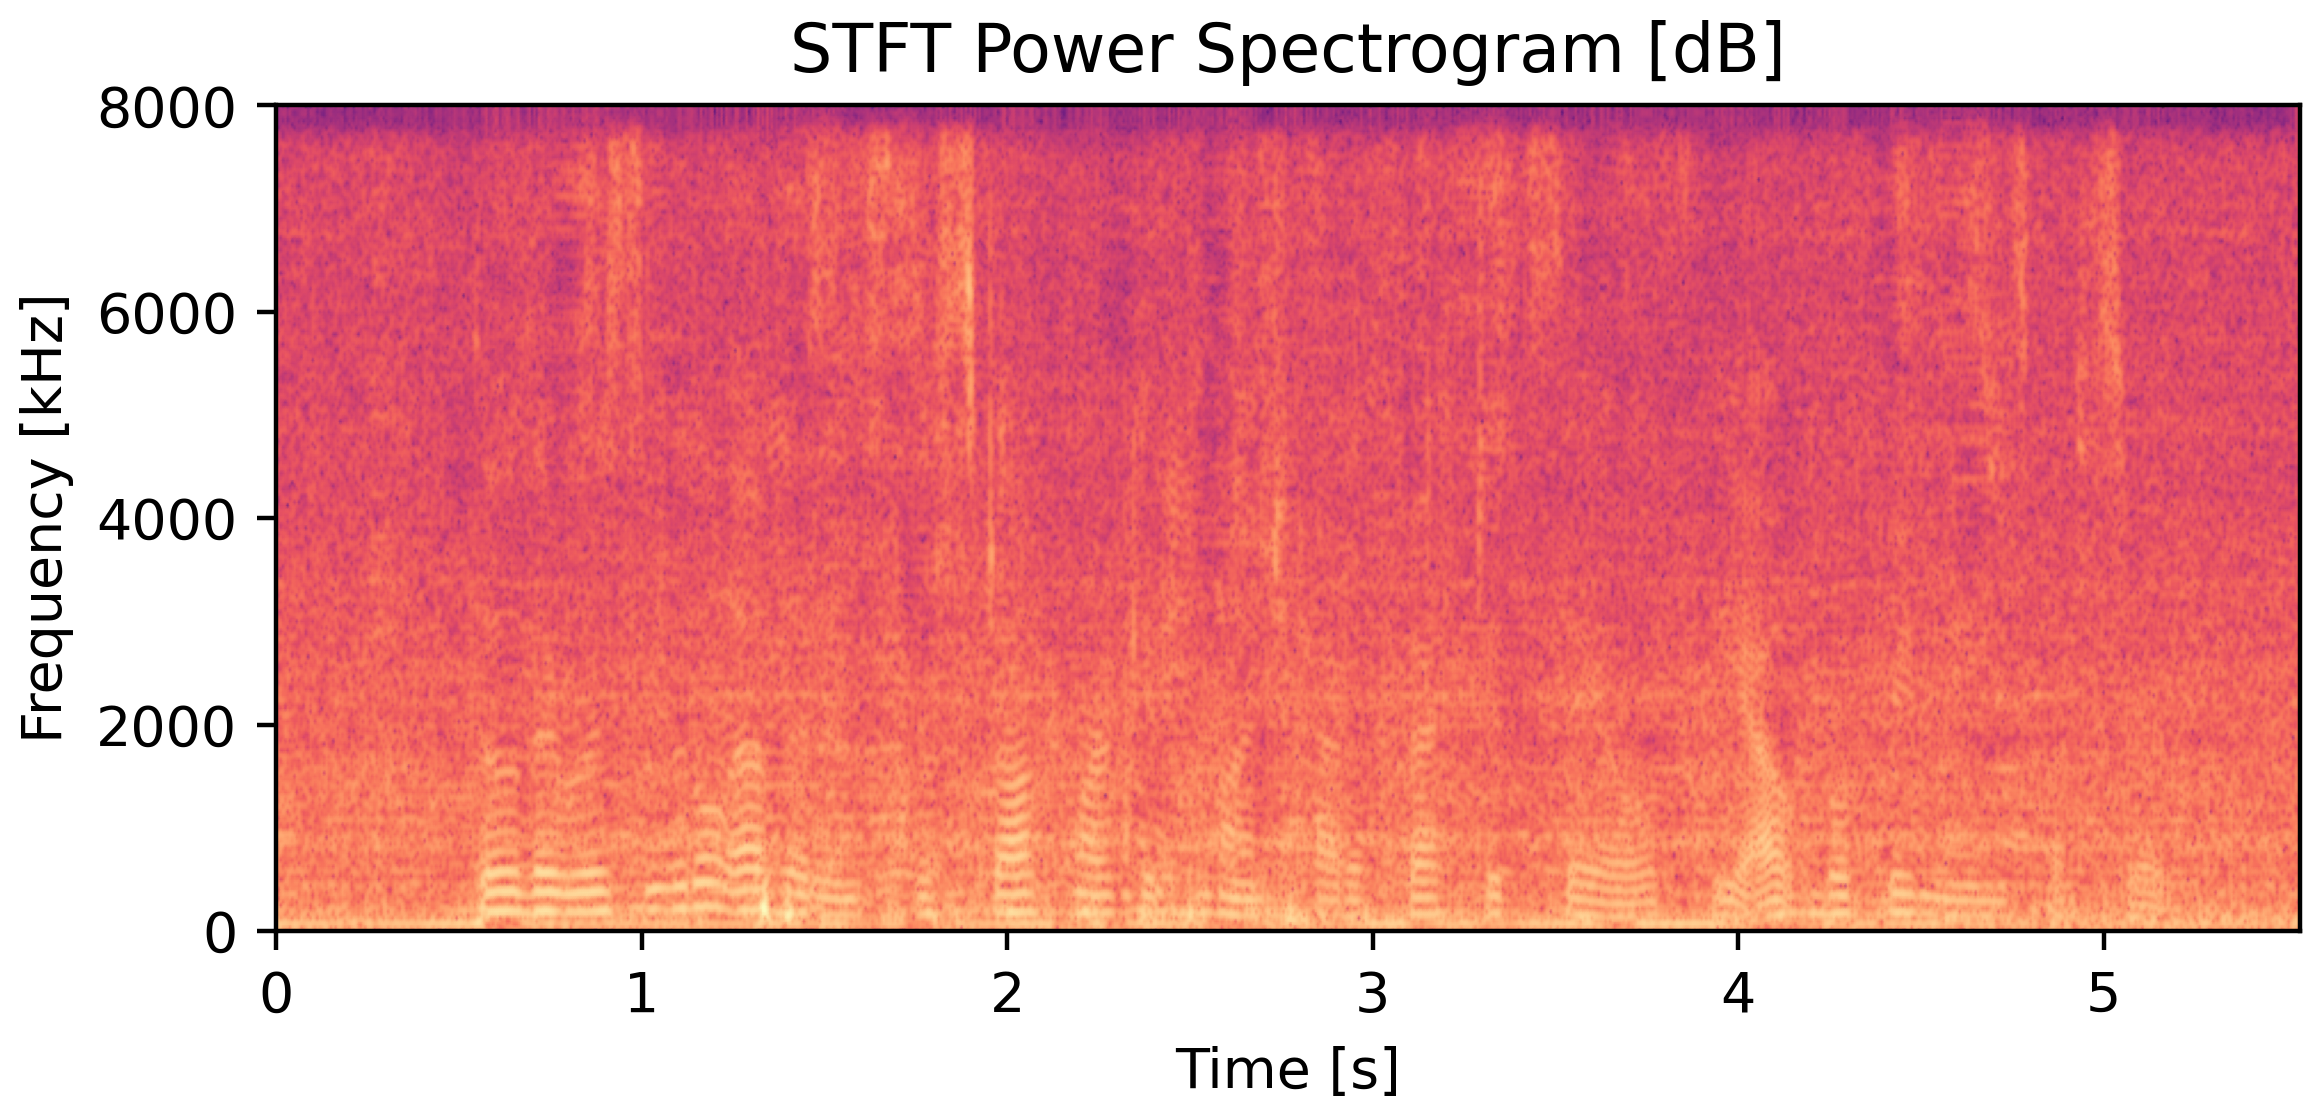
\includegraphics[width=\linewidth]{Features/images/noisy_specgram}
    \caption{Noisy mixture spectrogram}\label{fig:noisy_specgram}
\end{figure}
\begin{figure}[H]
    \centering
    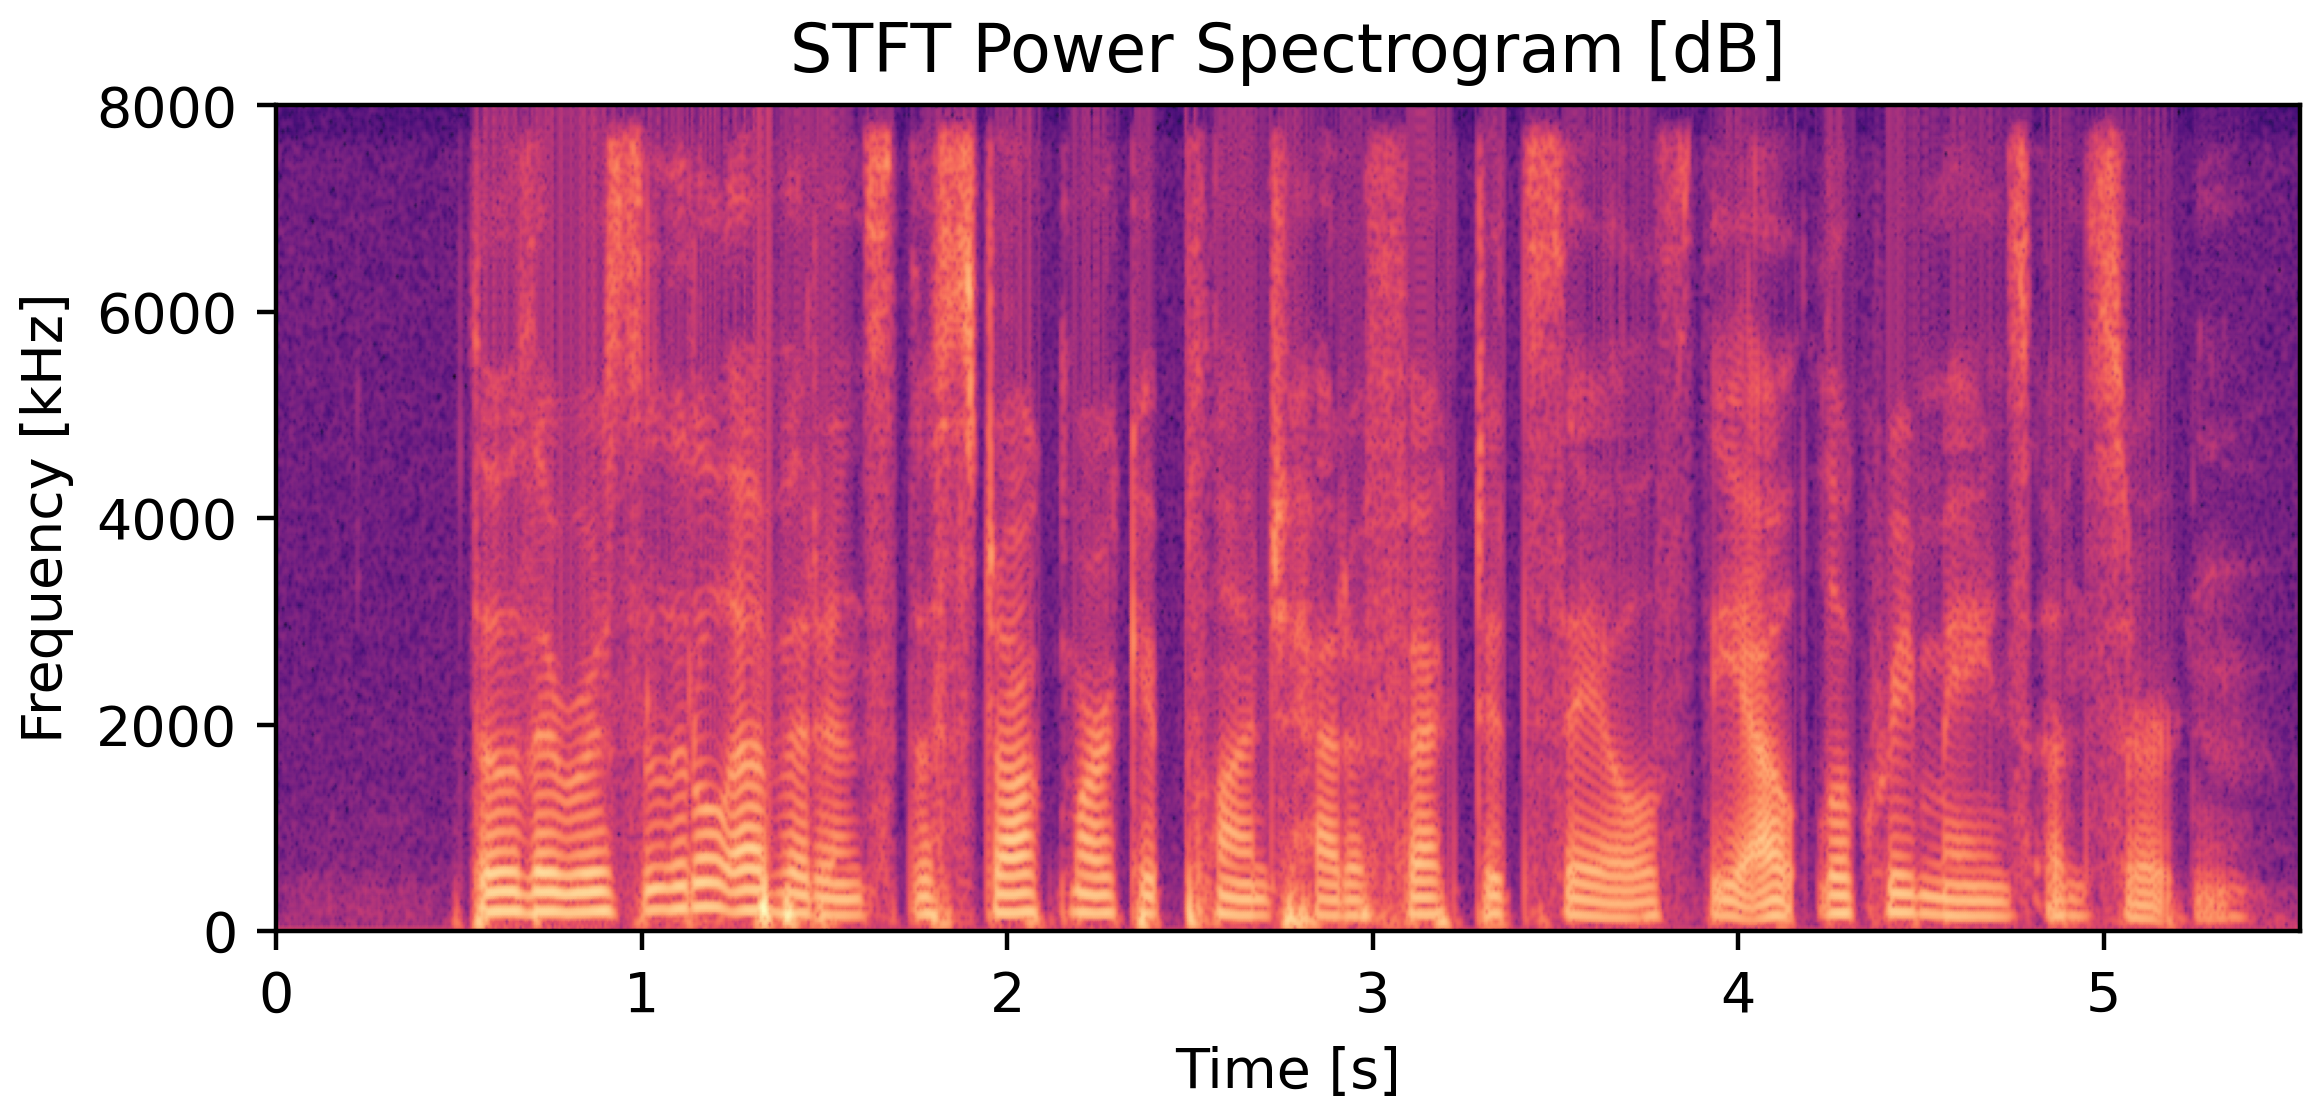
\includegraphics[width=\linewidth]{Features/images/clean_specgram}
    \caption{Reference clean speech spectrogram}\label{fig:clean_specgram}
\end{figure}

Examination of the T-F units provides a 
possibility to classify an entire unit
or parts of a unit 
as a speech-centric bin or, on the contrary, 
as interference (mainly noise). 
Based on this classification, 
appropriate weights are associated with each segment bin.
In that way, speech elements can be extracted 
by separating of the classified speech 
out of the mixture, or alternatively, 
the attenuation of non-speech elements 
in certain activity areas 
along the length of the audio signal.
In general, the association of weights for classifying different
elements in a signal is called T-F masking. 
This process of T-F masking takes a 
significant role in CASA and BSS applications, 
and in recent years, they proved to be 
very useful in E2E-ASR systems.

Additional use of T-F masking 
is to tie it as input to a beamformer that
in turn, filters interferences based 
on the classification received 
by the masking operation.

\section{IBM --- Ideal Binary Mask}
Assuming that a voice activity detection algorithm
can separate speech from noise effectively,
the IBM technique is based on power differences.
Whenever the speech's power 
spectral density (PSD) is higher 
than any of the interferences PSD, 
the speech is masked binarily to ``1''.
\begin{align}\label{eq:ibm_mask}
    \mathbf{M}_{s}(j\omega, t) & = 
        \begin{cases}
            1, & if\;|\mathbf{S}(t,j\omega)|^2 - |\mathbf{N}(t,j\omega)|^2 > \epsilon \\
            0, & otherwise
        \end{cases}
\end{align}
Where \(\epsilon\) marks a changeable threshold value 
for the speech activity detection over the noise.

Equation~\ref{eq:ibm_mask} indicates that as a result of 
applying the IBM masks, the speech and interference separated
sources become complementary in such a way that
\[\mathbf{M}_{n} = 1 - \mathbf{M}_{s} \] and thus:
\begin{align}
    y(t) &= \begin{cases}
        \hat{x_{s}}, &if\;\;\mathbf{M}_{s} = 1 \\
        \hat{x_{n}}, &if\;\;\mathbf{M}_{s} = 0
    \end{cases}
\end{align}

\section{IRM --- Ideal Ratio Mask}
% \begin{align}
%     \mathrm{IRM}(f;t) = \left( \frac{ || }{  } \right)
% \end{align}
Unlike IBM, where hard decisions in terms of 
boolean values are made,
that is, marking speech or noise 
elements with ``true'' or ``false'', the Ideal Ratio Mask (IRM) provides a soft decision
mechanism with values in the range of \([0,1]\)\cite{Jiang2018RobustBF}.
The IRMs at any T-F unit of the clean speech and noise artifacts,
\(\mathbf{M}_{s}(j\omega, t)\) and \(\mathbf{M}_{n}(j\omega, t)\),
are given in 
Equations\;\ref{eq:irm_speech} and \ref{eq:irm_noise}, respectively.

\begin{align}
    \label{eq:irm_speech}\mathbf{M}_{s}(j\omega, t) & = {\left( \frac{|\mathbf{S}(t,j\omega)|^2}{|\mathbf{S}(t,j\omega)|^2 + |\mathbf{N}(t,j\omega)|^2} \right)}^{\beta} \\
    \label{eq:irm_noise}\mathbf{M}_{n}(j\omega, t) & = {\left( \frac{|\mathbf{N}(t,j\omega)|^2}{|\mathbf{S}(t,j\omega)|^2 + |\mathbf{N}(t,j\omega)|^2} \right)}^{\beta}
\end{align}
 
Where \(\beta \) is a tunable parameter that 
controls the strength of the mask estimations. 
A value of 0.5 is used 
for a fair trade-off between speech and noise mask estimations.
%
\begin{align}
    \mathbf{M}_{s}(j\omega, t) & = \sqrt{\left( \frac{|\mathbf{S}(t,j\omega)|^2}{|\mathbf{S}(t,j\omega)|^2 + |\mathbf{N}(t,j\omega)|^2} \right)} \\
    \mathbf{M}_{n}(j\omega, t) & \approx 1 - \mathbf{M}_{s}
\end{align}

\begin{figure}[H]
    \centering
    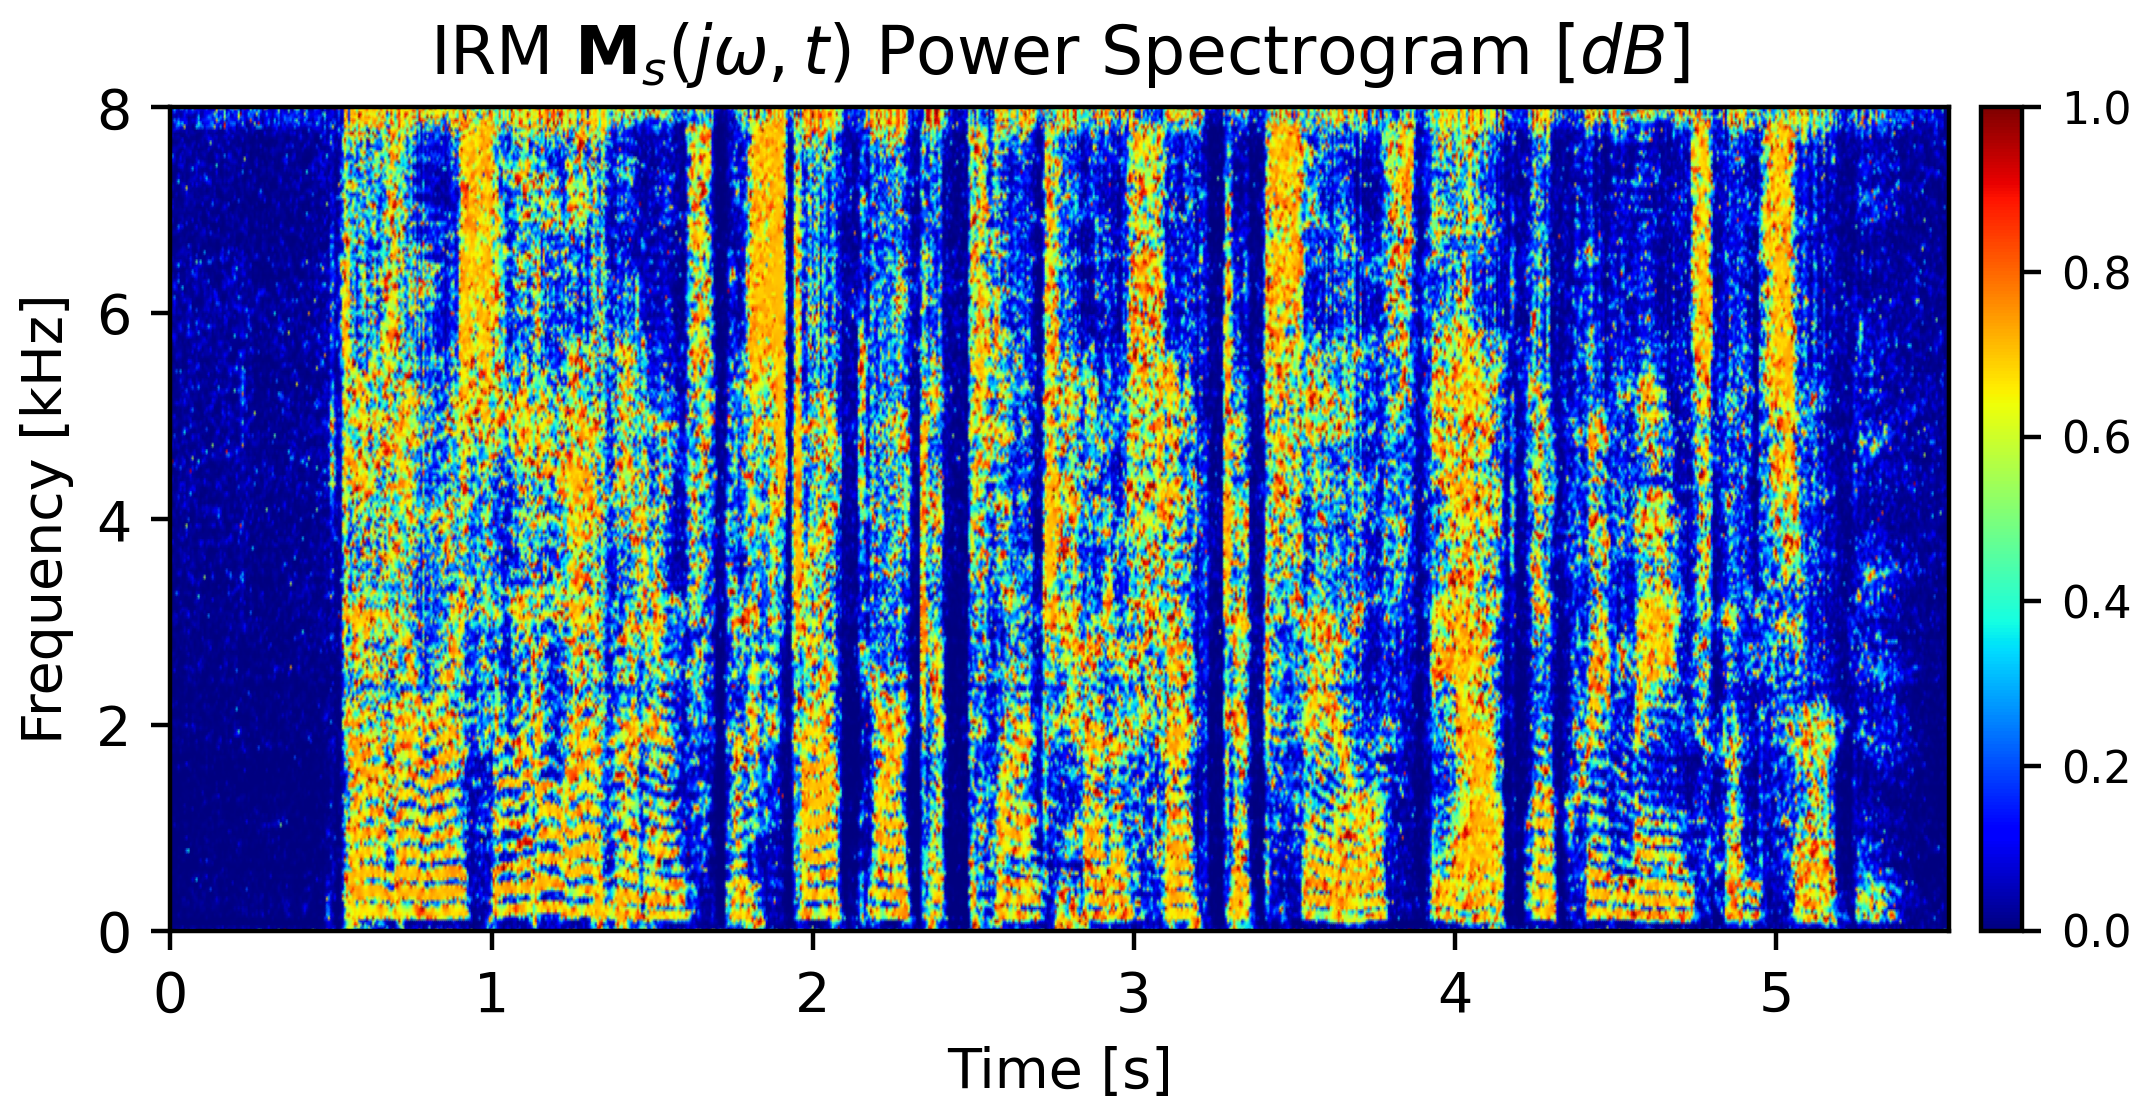
\includegraphics[width=\linewidth]{Features/images/irm_mask}
    \caption{IRM Speech Mask \(\mathbf{M}_{s}(j\omega, t)\)}\label{fig:irm_mask}
\end{figure}
\begin{figure}[H]
    \centering
    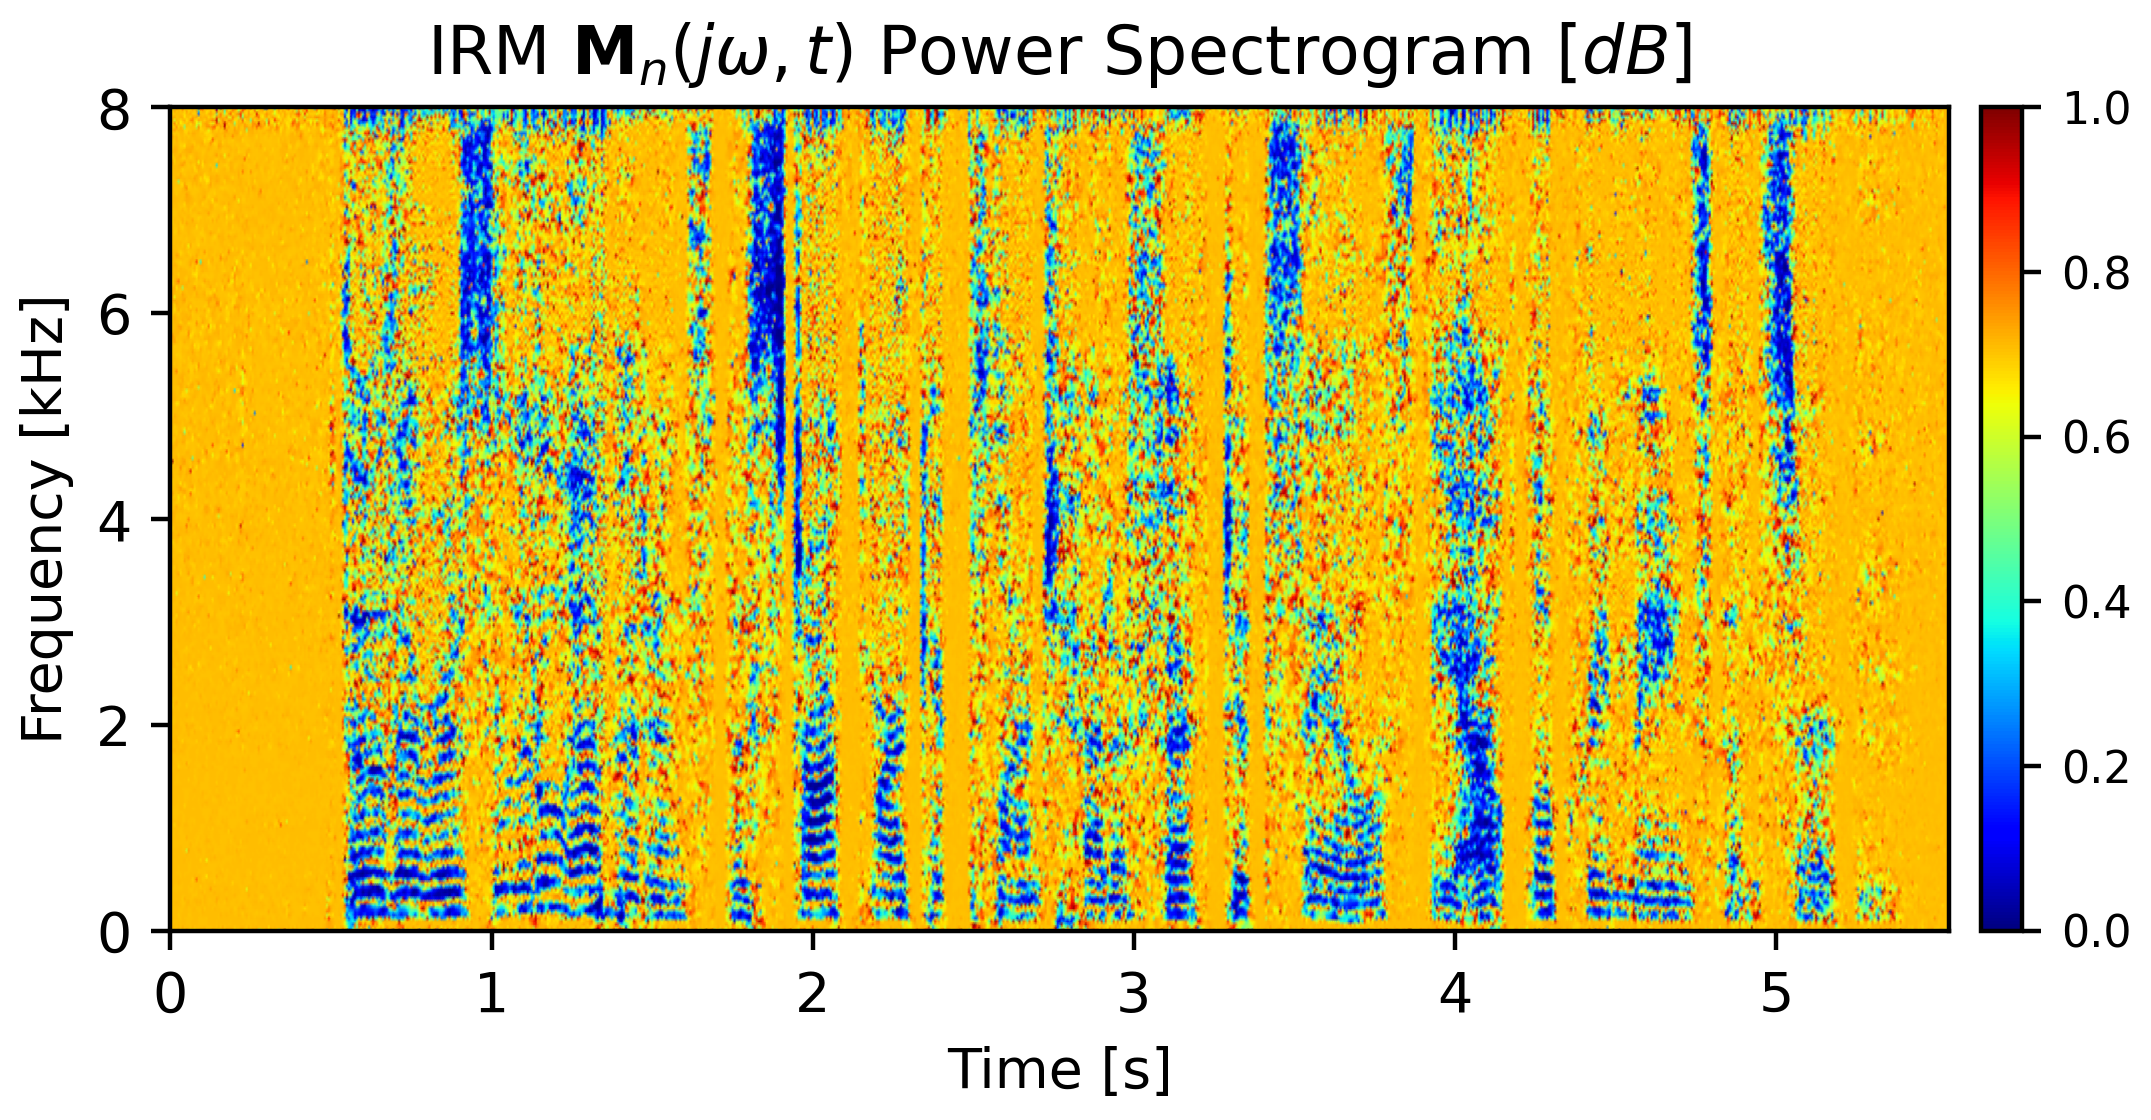
\includegraphics[width=\linewidth]{Features/images/irm_mask_noise}
    \caption{IRM Noise Mask \(\mathbf{M}_{n}(j\omega, t)\)}\label{fig:irm_mask_noise}
\end{figure}

%
Thus, the covariance matrices are extracted by:
\begin{align}
    \mathbf{R}_{NN}(j\omega) & = \frac{1}{\sum\limits_{t=1}^{T}\mathbf{M}_{n_{(jw, t)}}}\sum_{t=1}^{T}\mathbf{M}_{n_{(jw, t)}}|\mathbf{R}_{x_{(jw, t)}}|^2\\
    \mathbf{R}_{SS}(j\omega) & = \frac{1}{\sum\limits_{t=1}^{T}\mathbf{M}_{s_{(jw, t)}}}\sum_{t=1}^{T}\mathbf{M}_{s_{(jw, t)}}|\mathbf{R}_{x_{(jw, t)}}|^2
\end{align}

\subsection{Masks Estimations}
The IRM masks, \(\mathbf{M}_{s}(j\omega, t)\), \(\mathbf{M}_{n}(j\omega, t)\)
given in Equations\;\ref{eq:irm_speech}, \ref{eq:irm_noise} are bounded
in the range of [0, 1]. 
Since both the speech and noise masks are bounded in that range, it is easier
to use a Sigmoid activation function
as the output layer, 
thus ensuring the output indeed remains in this range.

A simple neural network of six to eight fully-connected (FC) layers,
as seen in Figure\;\ref{fig:irm_dnn}, is proposed for
classifying the input features to the desired IRM masks.
The network's input features are the MFCCs of the microphone-array.
Each input signal is framed into \(25ms\) lasting frames with a
hopping length of \(6.25ms\). With a sampling frequency of \(16KHz\), 
the framing settings are 400 samples per frame and 
a total of 300 overlapping samples. 

A BLSTM (Bidirectional Long Short-Term Memory)
layer is placed as the first block in the network,
giving weight to the temporal context as well.
In that way, three additional adjacent feature maps 
are concatenated from both sides of the currently 
processed T-F unit feature map.
The BLSTM is then followed 
by several fully connected (FC) layers 
holding in between the ReLU activation functions.

\begin{figure}[H]
    \centering
    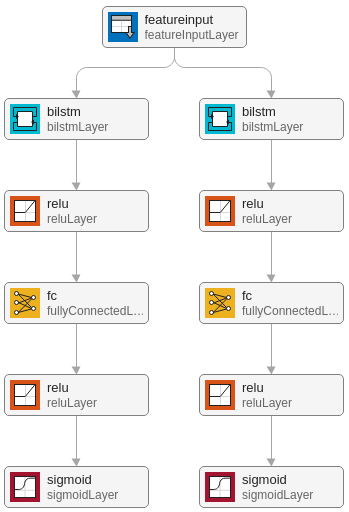
\includegraphics[width=0.95\linewidth]{Features/images/irm_dnn}
    \caption{IRM estimation DNN blocks diagram}\label{fig:irm_dnn}
\end{figure}

Production of both the speech and noise estimations co-occurs. 
Consequently, the cost function should 
consider the two masks in the 
minimization process of the error term.
To that end, the cost function is defined as:
\begin{align}
    \ell(\mathbf{\widehat{M}}_{j\omega, t},\;\mathbf{M}_{j\omega, t}) & = 
        \frac{1}{2N}\sum_{j\omega, t}
        \left[ 
            \beta\!\left( 
                \mathbf{\widehat{M}}^{(s)}_{j\omega, t} - 
                \mathbf{M}^{(s)}_{j\omega, t} 
            \right)^{2} 
            + \left( 1- \beta \right)\!
            \left(
                \mathbf{\widehat{M}}^{(n)}_{j\omega, t} - 
                \mathbf{M}^{(n)}_{j\omega, t} 
            \right)^{2} 
        \right]
\end{align}
Here, \(\beta\) denotes the weighing factor.
For a fair and evenly consideration between the masks, \(\beta \)
is set to 0.5.

The proposed IRM estimation network blocks diagram is shown in 
Figure\;\ref{fig:irm_nn}.

\begin{figure}[H]
    \centering
    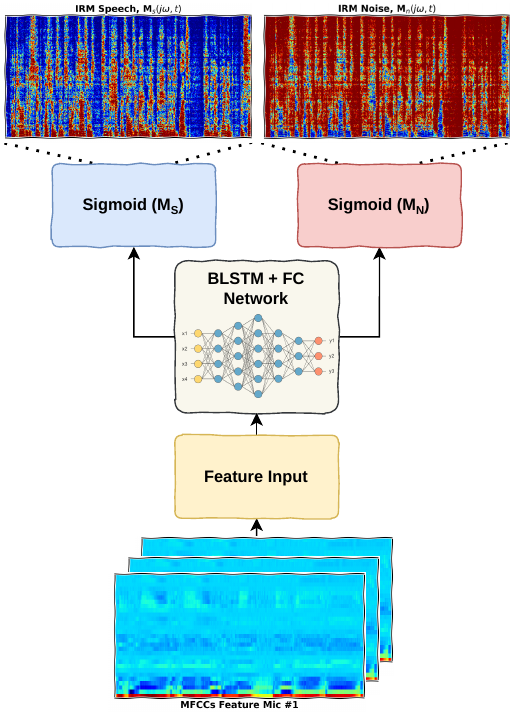
\includegraphics[width=0.75\linewidth]{Beamformers/images/irm_nn}
    \caption{Proposed DNN for IRM T-F masking estimations}\label{fig:irm_nn}
\end{figure}


\begin{figure}[H]
    \centering
    \subfloat[\label{irm_s_ref}]{%
       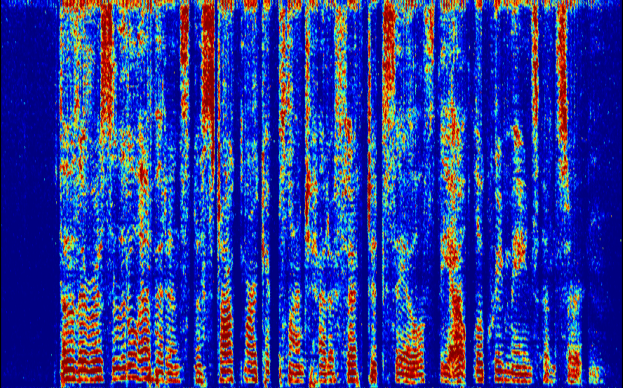
\includegraphics[width=0.45\linewidth]{Beamformers/images/irm_s_ref}}
    \hspace{0.1cm}
    \subfloat[\label{irm_s_nn}]{%
        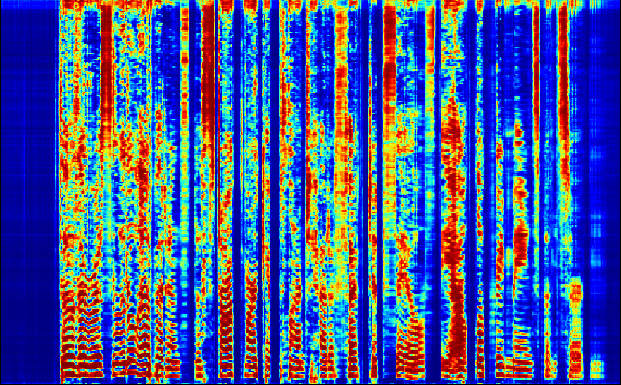
\includegraphics[width=0.45\linewidth]{Beamformers/images/irm_s_nn}}
    \vspace{-0.35cm}
    \subfloat[\label{irm_n_ref}]{%
        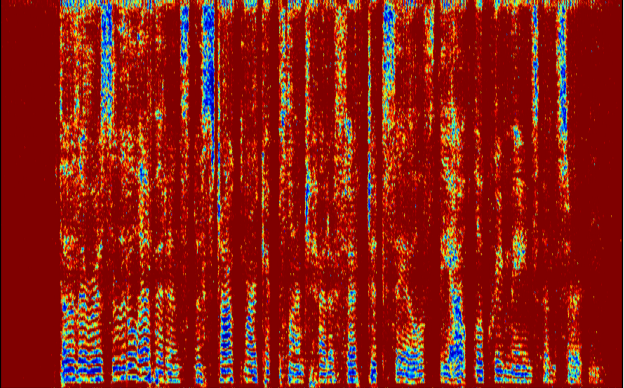
\includegraphics[width=0.45\linewidth]{Beamformers/images/irm_n_ref}}
    \hspace{0.1cm}
    \subfloat[\label{irm_n_nn}]{%
        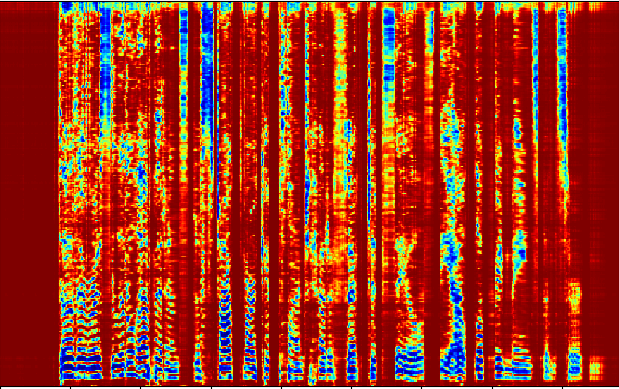
\includegraphics[width=0.45\linewidth]{Beamformers/images/irm_n_nn}}
        \caption{(a) and (b) are the ``IRM'' 
        reference vs. estimation masks of the speech.
        \(\mathbf{\widehat{M}}^{(s)}_{j\omega, t}\), \(\mathbf{M}^{(s)}_{j\omega, t}\);\;\;
        (c) and (d) are the ``IRM'' reference vs. estimation masks 
        of the noise \(\mathbf{\widehat{M}}^{(n)}_{j\omega, t}\), \(\mathbf{M}^{(n)}_{j\omega, t}\).}\label{fig:irm_ref_s_n} 
\end{figure}


\subsection{Measurements}
\subsubsection{SNR}
\begin{figure}[H]
    \centering
    \subfloat[\label{irm_enh_snr}]{%
       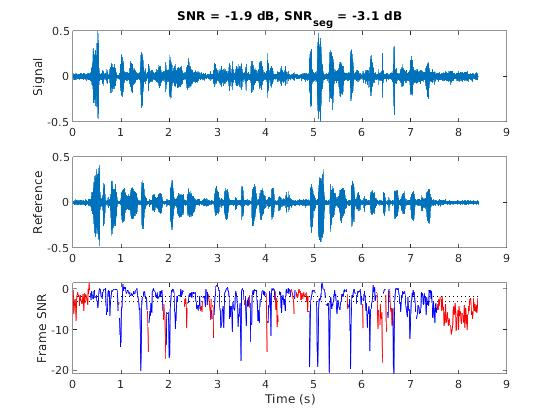
\includegraphics[width=0.5\linewidth]{Features/images/irm_enh_snr}}
    % \hspace{0.1cm}
    \subfloat[\label{irm_noisy_snr}]{%
        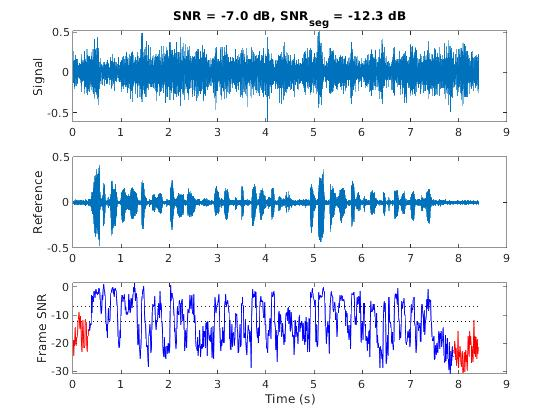
\includegraphics[width=0.5\linewidth]{Features/images/irm_noisy_snr}}
    \caption{(a) ``IRM'' enhanced SNR \& Segmental-SNR degradation
        with respect to the clean reference speech;\;\;
        (b) The SNR \& Segmental-SNR ratios between the
        clean reference speech and the noisy mixture.}\label{fig:irm_enh_noisy_snr} 
\end{figure}

Figure\;\ref{fig:irm_enh_noisy_snr} shows two measurements of the SNR \&
Segmental-SNR metrics for two subject signals, 
an ``IRM'' enhanced beamformed
version of the noisy mixture and the noisy mixture itself
with respect to the clean reference speech.
The overall improvements in SNR and Segmental-SNR 
are the ratios between the enhanced beamformed signal
and the noisy mixture. Thus, from Figure\;\ref{fig:irm_enh_noisy_snr}
the accumulated improvement in SNR is:
\[|SNR_{noisy}| - |SNR_{enh}| = 5.1725\;[dB]\]
Likewise, the improvement in Segmental-SNR is \(9.2675\;[dB]\).
It is important to note that the enhanced beamformed signal
does not align in time with the clean speech reference. 
In a worst-case scenario, we measured a delay of \(-0.0014\;[s]\),
which equals approximately \(22\) samples. 
A perfectly aligned comparison considers being more 
accurate, but since the frame lengths' (400 samples)
are much larger than the worst measured delay, 
the impact of this time misalignment is less acute.
The Segmental-SNR calculation involves 
a VAD (voice activity detection) algorithm
for dropping segments where the detected speech activity is negligible.
These dropped segments are red colored in Figure\;\ref{fig:irm_enh_noisy_snr}.

\begin{figure}[H]
    \centering
    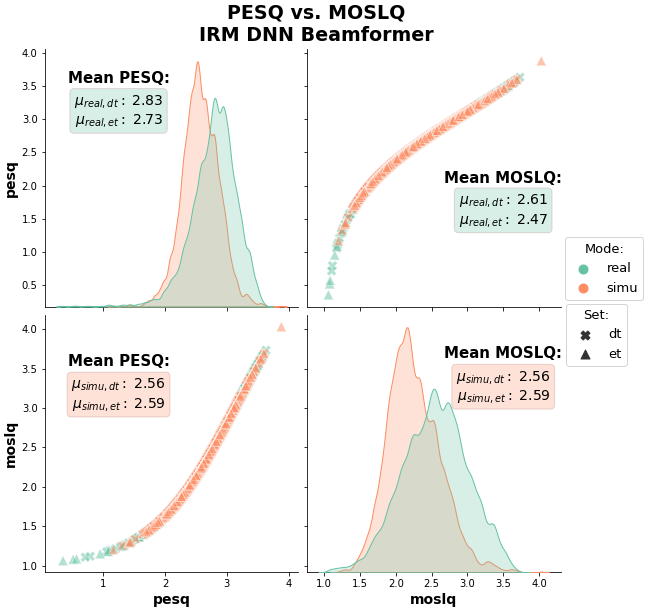
\includegraphics[width=\linewidth]{Experiments/images/irm_pesq_mosq}
    \caption{IRM beamformer PESQ vs. MOSLQ}\label{fig:irm_pesq_mosq}
\end{figure}

In Figure\;\ref{fig:irm_pesq_mosq} presented the ``PESQ'' and ``MOSLQ'' 
metrics for the IRM beamformer. The results are shown in a pair-plot
diagram, where the correlations between each pair of metrics are plotted.
On the diagonal, the distributions of the measured values are shown.
On top of the plots also shown are the mean values for both 
the ``PESQ'' and ``MOSLQ'' under the test cases of the real and 
simulation datasets from the ``CHiME4'' dataset. ``et'' stands for
the evaluation subset and ``dt'' marks the development subset.
More details about the datasets are provided in Chapter\;\ref{ch:datasets}.

A strong correlation between the ``PESQ'' and ``MOSLQ'' is seen in the
plot, and this behavior is both understandable and desirable since
the ``MOSLQ'' metric is based on the ``PESQ'' measurement.

Another pair-plot for the SNR, ``Segmental-SNR'', ``SI-SNR'' and ``STOI''
metrics is shown in Figure\;\ref{fig:irm_snr_stoi}.
The ``simulation'' subset yields better results in terms of
performance. It is important to note that faulty microphones
in the ``real'' subset are dropped prior to taking the measurements.
Nevertheless, the ambient noise absorbed is characterized by
a real scenario and a non-artificial room impulse response. On the other hand,
the ``simulation'' subset is composed of a recording taken in a relatively
clean environment (recording booth) and an artificial mixture of
the recorded background noises.

Because the SNR and Segmental-SNR are measured as the improvement
compared to the noisy mixture, 
and since the background noises are truncated 
to match the booth recorded speech for the ``simulation'' subset, 
the results for those metrics are more sparsely distributed 
compared to the ``real'' subset measurements. 
With the ``SI-SNR'', 
the measurements are taken regardless of the noisy mixture. 
Hence, the ``simulation'' results are far better 
and more spatially dense 
in contrast to the ``real'' subset ``SI-SNR'' results.

Likewise, in the same manner, 
the ``STOI'' is measured regardless of the noisy mixture
but relatively to the clean speech. 
Therefore, the ``simulation'' 
subset distribution is narrower with lower variance.

% The results are summarized in Table\;\ref{tbl:irm_snr_stoi},
% side by side with the ideal masks and the improvement ratios.

\begin{figure}[H]
    \centering
    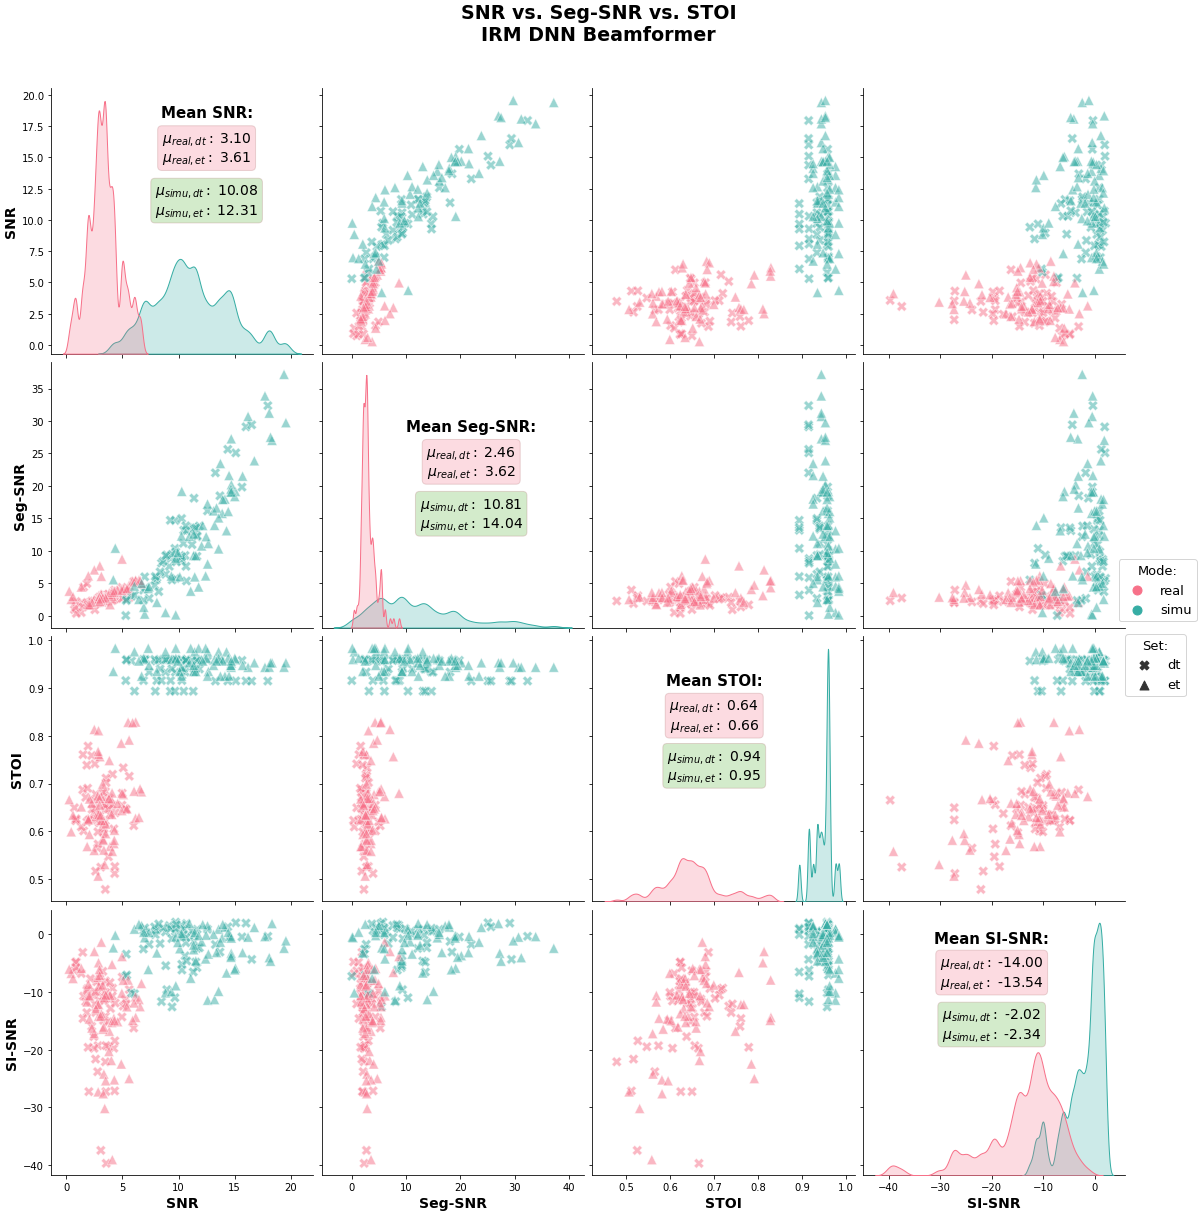
\includegraphics[width=\linewidth]{Features/images/irm_snr_stoi}
    \caption{IRM beamformer SNR vs. Segmental-SNR vs. STOI vs. SI-SNR}\label{fig:irm_snr_stoi}
\end{figure}

In order to evaluate the generalization of the prediction model,
the DNN estimations are compared to the ideal mask enhancement.
In Figure\;\ref{fig:irm_ideal_snr}, shown is the measurements of 
the SNR and ``Segmental-SNR'' for an ideal IRM mask.
SNR measurement.

\begin{figure}[H]
    \centering
    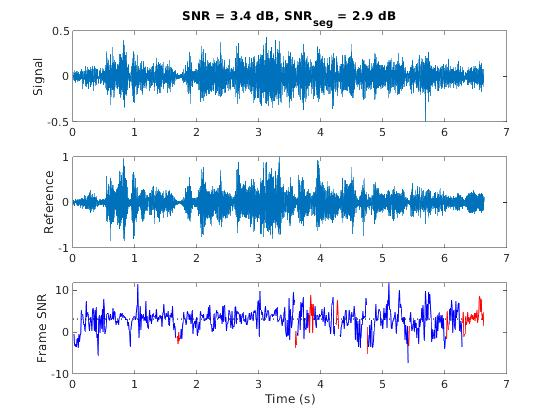
\includegraphics[width=\linewidth]{Features/images/irm_ideal_snr}
    \caption{Ideal IRM beamformer enhancement SNR \& Segmental-SNR.}\label{fig:irm_ideal_snr}
\end{figure}



\section{cIRM --- Complex Ideal Ratio Mask}\label{ssec:cirm}
Both IBM and IRM utilize the noise and speech magnitudes only
while completely neglecting the phase arguments.
The outcome of the STFT operation is a complex pair
representation of each T-F unit. Recent studies
showed the importance of 
the phase element in 
speech seperation\cite{7364200,Xia2017UsingOR}.

In that manner, further extension of the IRM mask 
to include the imaginary part 
altogether with the magnitudes forms the cIRM. 
Thus, instead of having a magnitude only based mask matrix, a complex
pair of masking matrices that make use of the phase element too is given.

The mixture \(y(t)\) after being processed by
the STFT operation can be described as a complex sum
whether in polar coordinates as seen in Equation\ref{eq:ystft_polar}
or in the general form as in Equation\ref{eq:ystft_general}.
\begin{align}\label{eq:ystft_polar}
    \mathbf{Y}(j\omega, t)  & = \mathcal{STFT} \{ y(t) \} := \mathbf{Y}_{j\omega, t} \nonumber \\
                            & = |\mathbf{A}_{_{\mathbf{Y}}}|\cos(\bm{\theta}_{_{\mathbf{Y}}}) 
                            + j|\mathbf{A}_{_{\mathbf{Y}}}|\sin(\bm{\theta}_{_{\mathbf{Y}}}) \\
\label{eq:ystft_general}      & = \mathbf{Y}_{r} + j\mathbf{Y}_{i}
\end{align}

The real and imaginary parts can be summarized as:
\begin{align}
    \mathbf{Y}_{r} & := \mathfrak{R}_{_{\mathfrak{C}}} \{\mathbf{Y}_{j\omega, t}\} 
                            = |\mathbf{A}_{_{\mathbf{Y}}}|\cos(\bm{\theta}_{_{\mathbf{Y}}})  \\
    \mathbf{Y}_{i} & := \mathfrak{T}_{_{\mathfrak{M}}} \{\mathbf{Y}_{j\omega, t}\} 
                            = |\mathbf{A}_{_{\mathbf{Y}}}|\sin(\bm{\theta}_{_{\mathbf{Y}}})
\end{align}
Extraction of the magnitude and phase from the complex representation 
is accomplished by the following set of 
Equations\ref{eq:complex_mag},\ref{eq:complex_phase}:
\begin{align}\label{eq:complex_mag}
    |\mathbf{A}_{_{\mathbf{Y}}}|    & = \sqrt{ \mathfrak{R}_{_{\mathfrak{C}}} \{\mathbf{Y}_{j\omega, t}\}^{2}
                                            + \mathfrak{T}_{_{\mathfrak{M}}} \{\mathbf{Y}_{j\omega, t}\}^{2} } \\
    \label{eq:complex_phase}\bm{\theta}_{_{\mathbf{Y}}}     & = \tan^{-1} \Bigg\{ \frac{ \mathfrak{T}_{_{\mathfrak{M}}} \{\mathbf{Y}(j\omega, t)\} }
                                            {\mathfrak{R}_{_{\mathfrak{C}}} \{\mathbf{Y}(j\omega, t)\}} \Bigg\}
\end{align}
Rearranging the equations above, 
we can write the cIRM mask's real and 
imaginary parts as:
\begin{align}
    \mathbf{M}_{r} & = \frac{\mathbf{Y}_{r}\mathbf{S}_{r} + \mathbf{Y}_{i}\mathbf{S}_{i}}
                            { \mathbf{Y}_{r}^{2} + \mathbf{Y}_{i}^{2}} \\
    \mathbf{M}_{i} & = \frac{\mathbf{Y}_{r}\mathbf{S}_{i} - \mathbf{Y}_{i}\mathbf{S}_{r}}
                            { \mathbf{Y}_{i}^{2} + \mathbf{S}_{r}^{2}}
\end{align}
Thus, the complex masks for the speech and noise are: 
\begin{align}
    \mathbf{M}^{(s)}_{j\omega, t} & = \mathbf{M}^{(s)}_{r} + j\mathbf{M}^{(s)}_{i} \nonumber \\
            & = \frac{\mathbf{Y}_{r}\mathbf{S}_{r} + \mathbf{Y}_{i}\mathbf{S}_{i}}
            { \mathbf{Y}_{r}^{2} + \mathbf{Y}_{i}^{2}} 
            + j \frac{\mathbf{Y}_{r}\mathbf{S}_{i} - \mathbf{Y}_{i}\mathbf{S}_{r}}
            { \mathbf{Y}_{i}^{2} + \mathbf{S}_{r}^{2}} \label{eq:cirmr_mask} \\
    \mathbf{M}^{(n)}_{j\omega, t} & = \mathbf{M}^{(N)}_{r} + j\mathbf{M}^{(N)}_{i} \nonumber \\
    & = \frac{\mathbf{Y}_{r}\mathbf{N}_{r} + \mathbf{Y}_{i}\mathbf{N}_{i}}
    { \mathbf{Y}_{r}^{2} + \mathbf{Y}_{i}^{2}} 
    + j \frac{\mathbf{Y}_{r}\mathbf{N}_{i} - \mathbf{Y}_{i}\mathbf{N}_{r}}
    { \mathbf{Y}_{i}^{2} + \mathbf{N}_{r}^{2}} \label{eq:cirmi_mask}
\end{align}
Therefore, applying a cIRM T-F masking requires a complex multiplication
for separation as opposed to the more basic IBM and IRM 
where magnitudes multiplications are taken in the real domain only.

The reference compressed cIRM masks are 
shown in Figure\;\ref{fig:cirm_ref_s_n};

\begin{figure}[H]
    \centering
    \subfloat[\label{cIRM_real_mask}]{%
       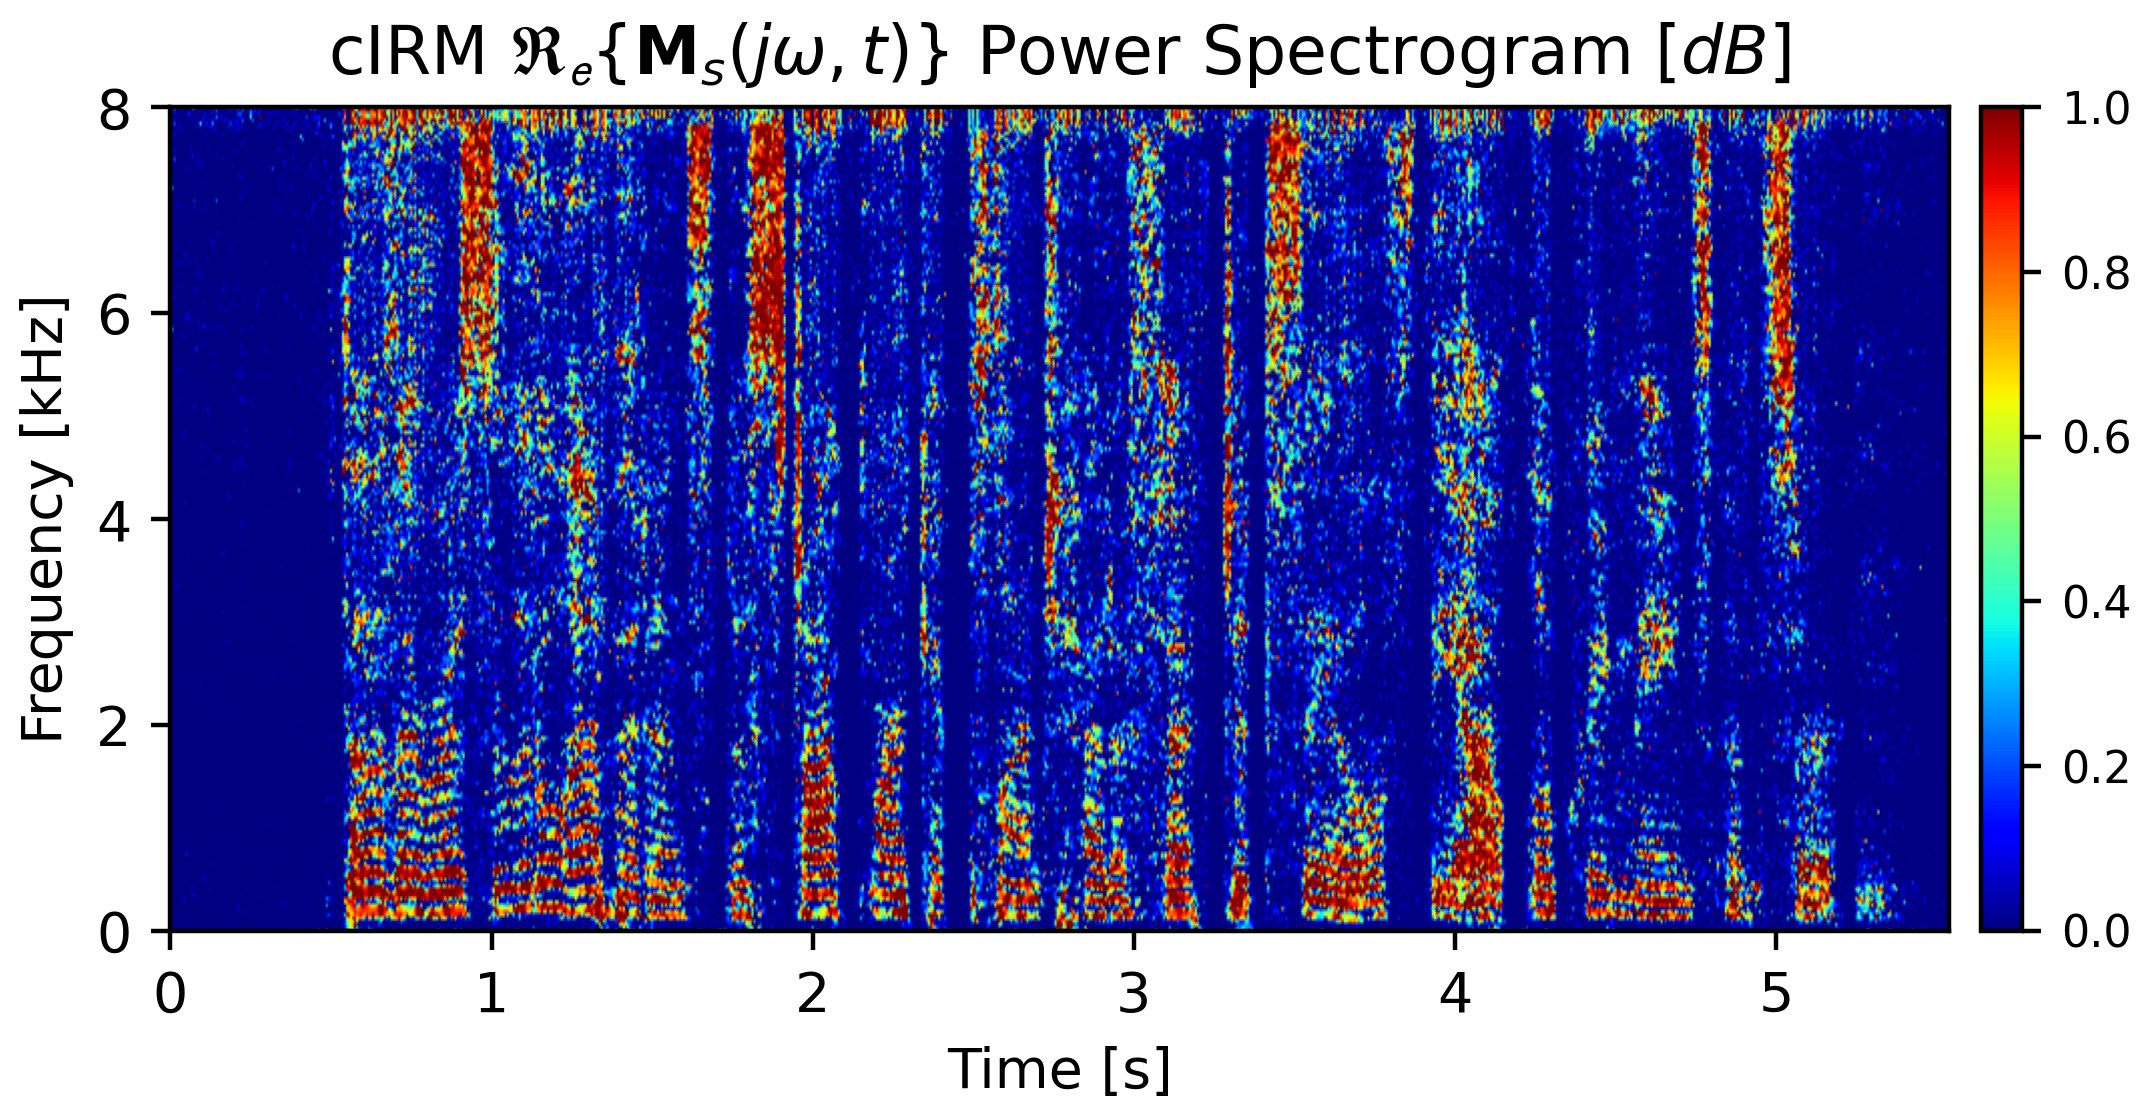
\includegraphics[width=0.45\linewidth]{Features/images/cIRM_real_mask}}
    \subfloat[\label{cIRM_imag_mask}]{%
        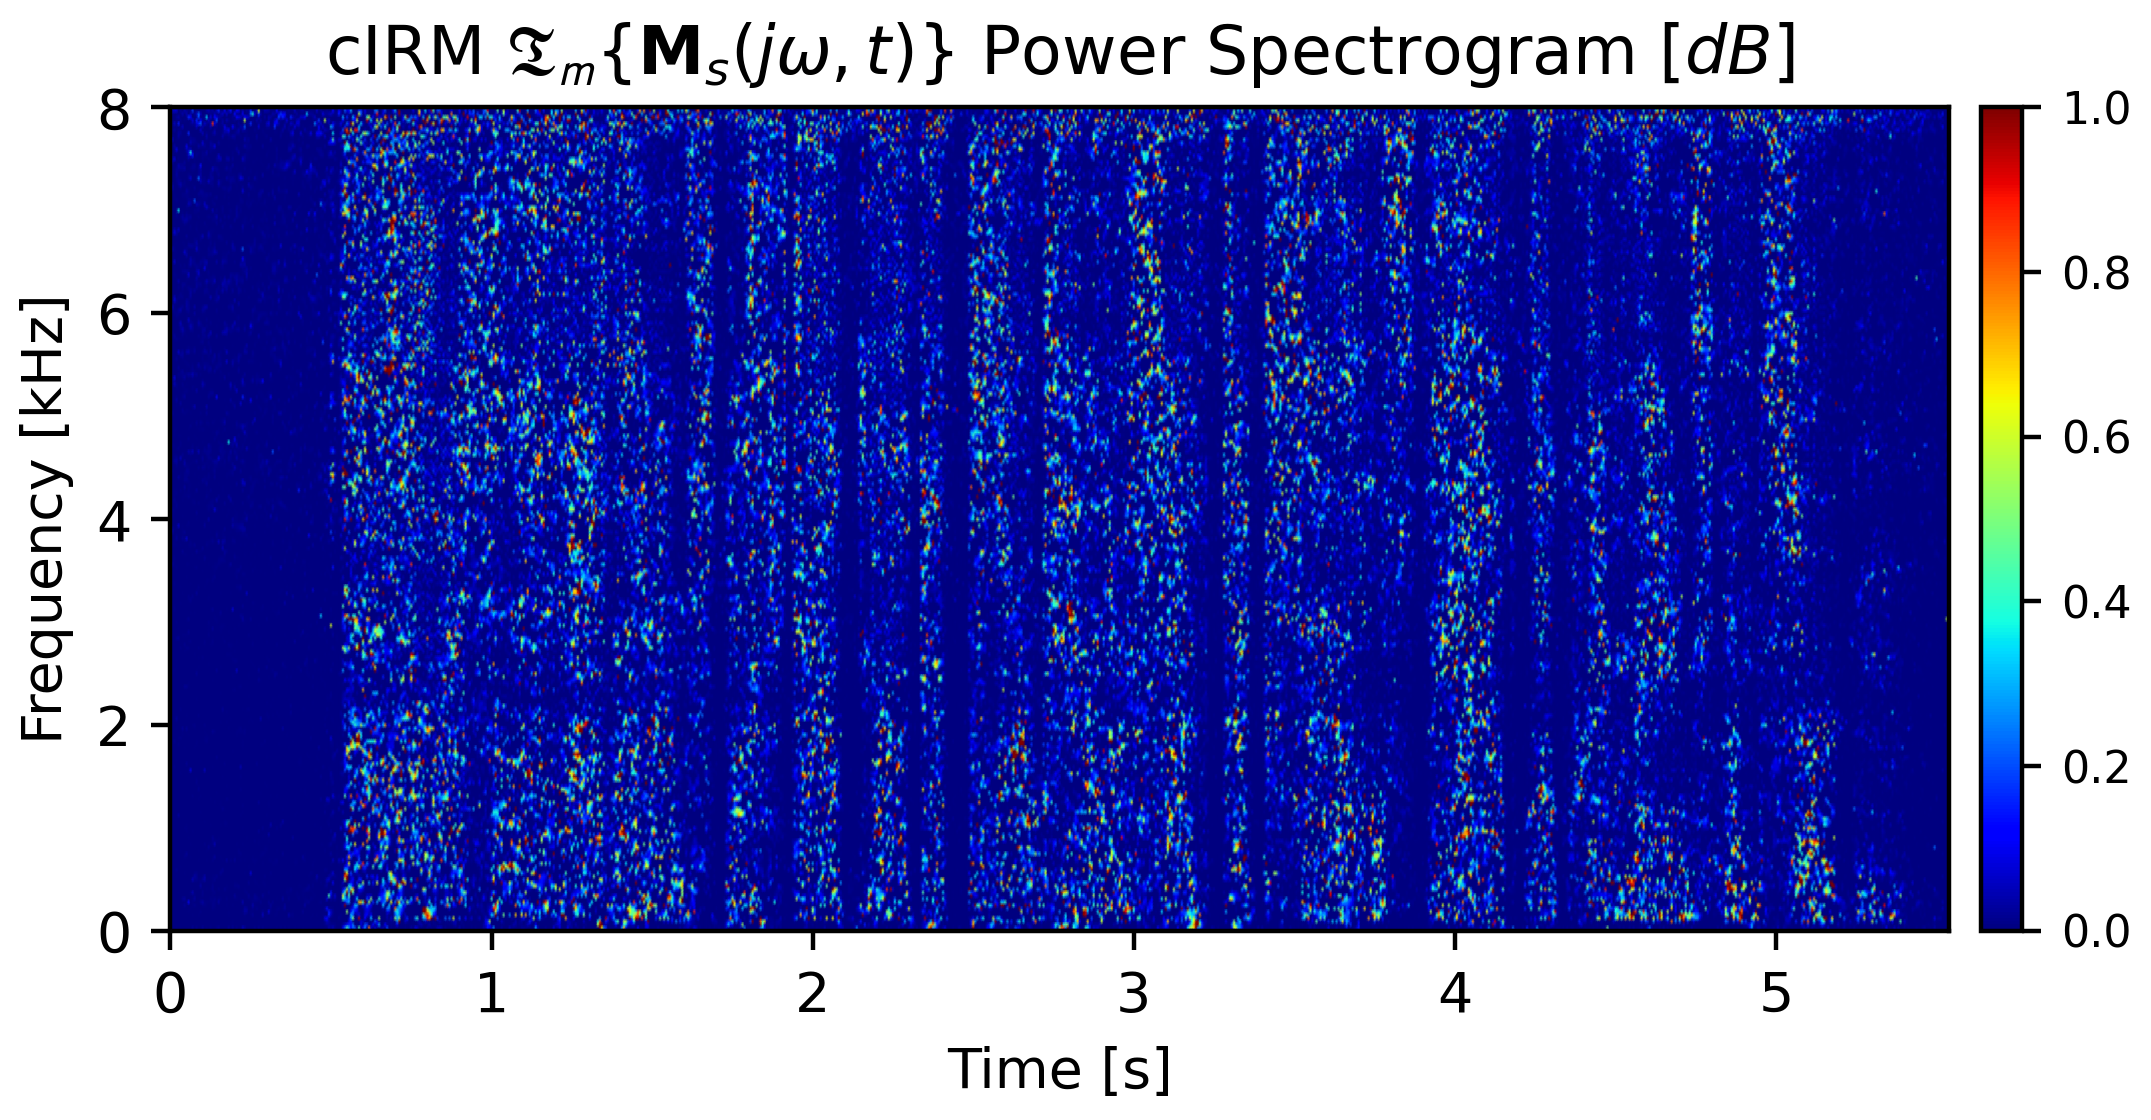
\includegraphics[width=0.45\linewidth]{Features/images/cIRM_imag_mask}}
    \vspace{-0.35cm}
    \subfloat[\label{cIRM_real_noise_mask}]{%
        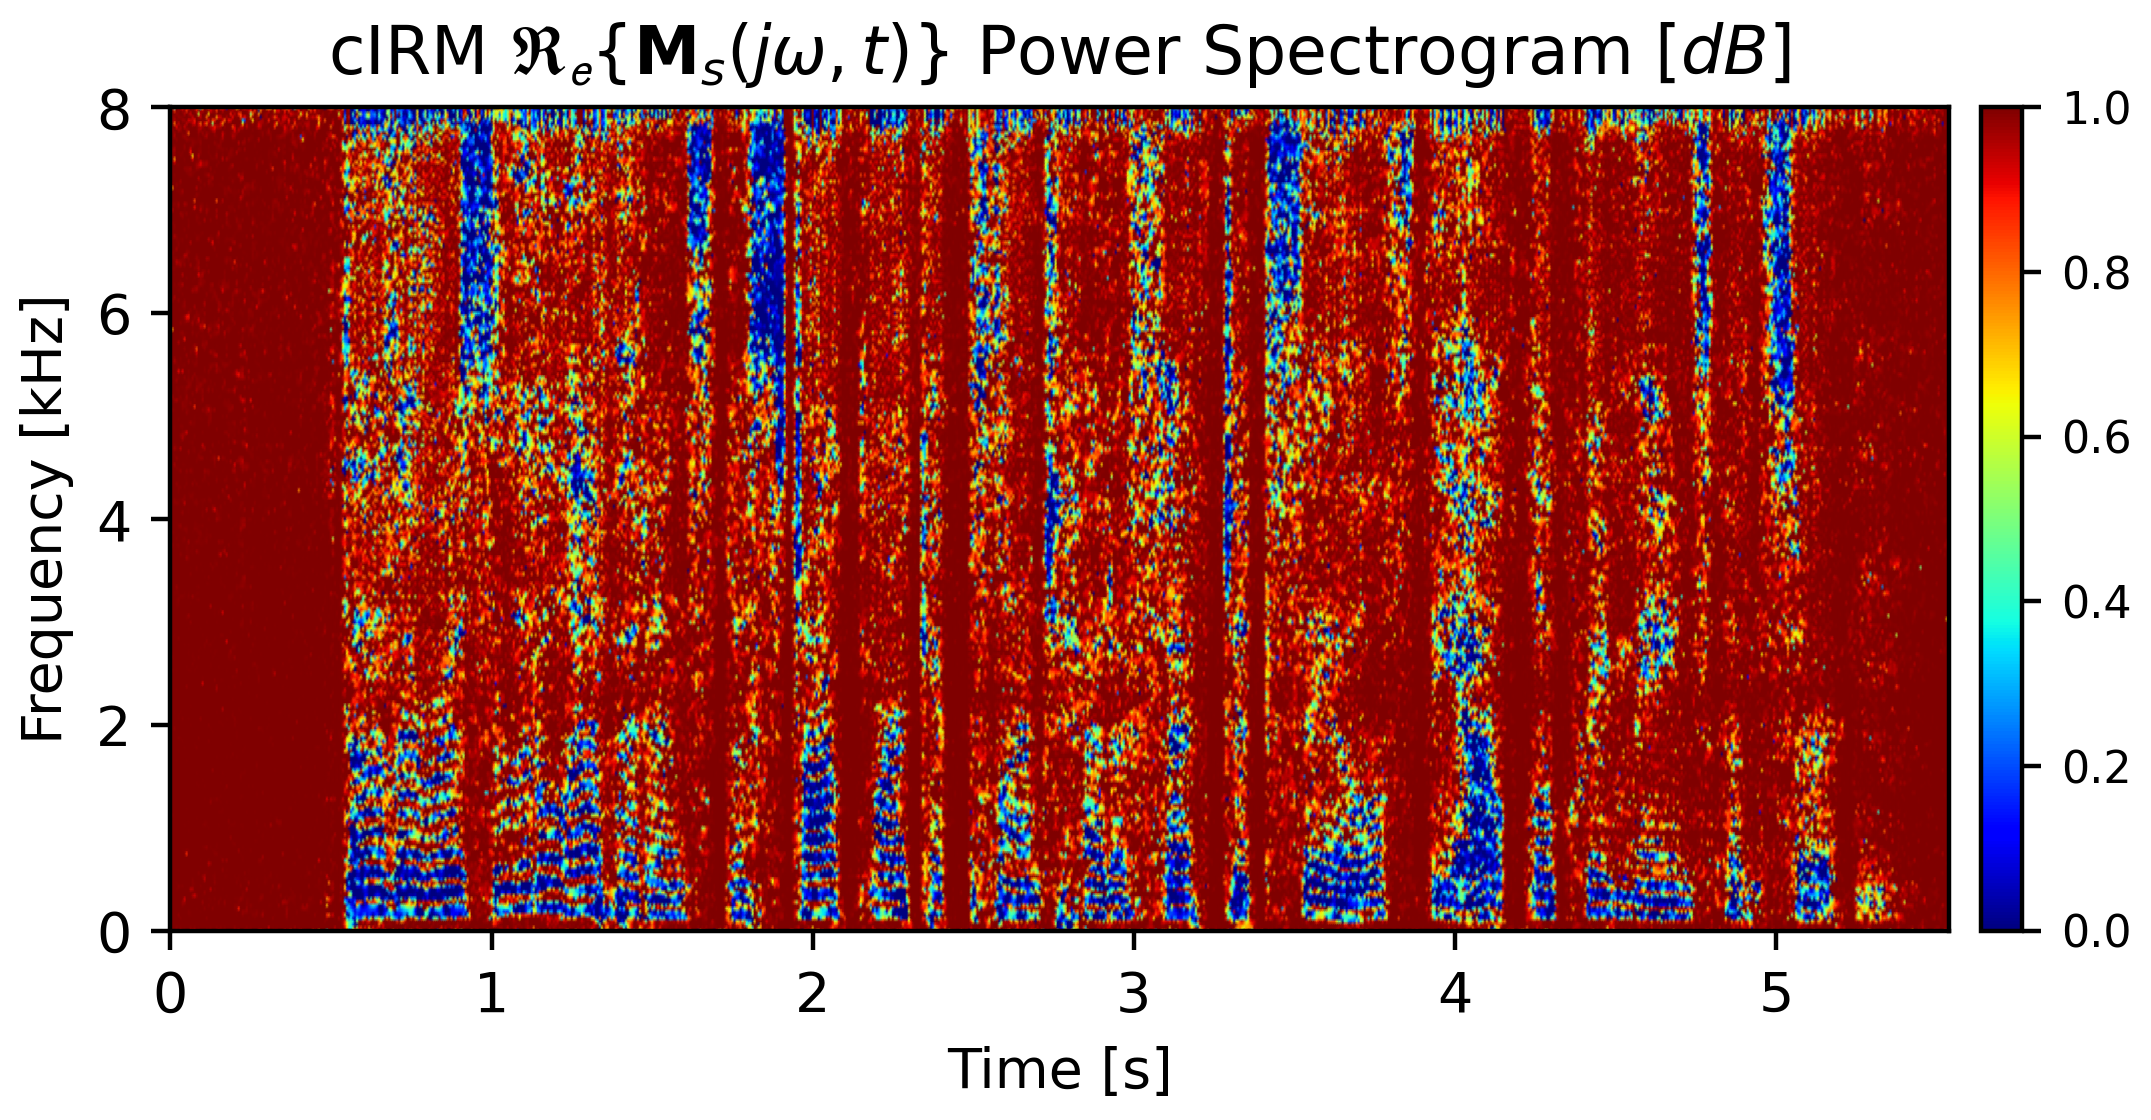
\includegraphics[width=0.45\linewidth]{Features/images/cIRM_real_noise_mask}}
    \subfloat[\label{cIRM_imag_noise_mask}]{%
        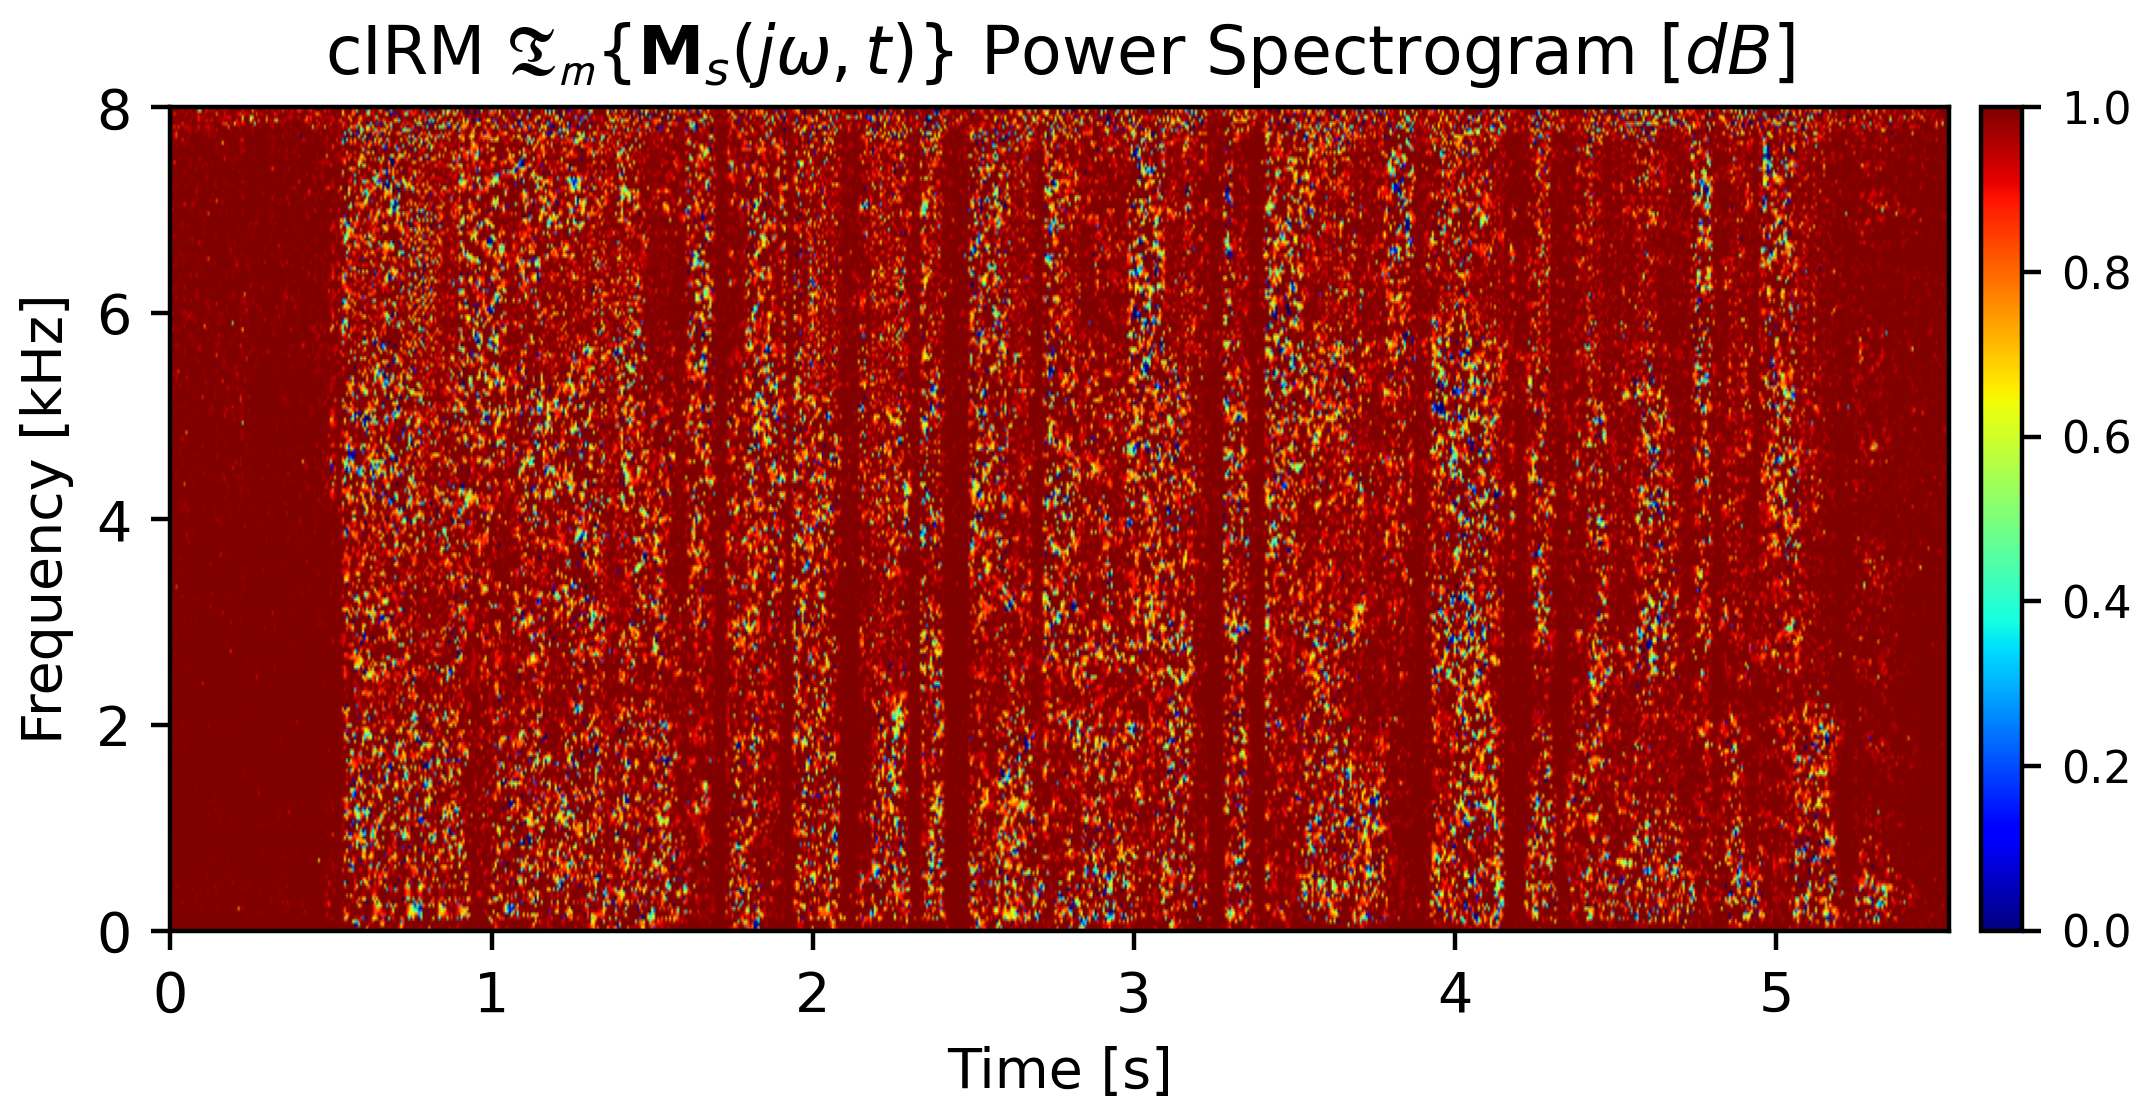
\includegraphics[width=0.45\linewidth]{Features/images/cIRM_imag_noise_mask}}
        \caption{(a) and (b) are the cIRM
        real and imaginary references of the speech 
        \(\mathbf{M}^{(s)}_{r}\), \(\mathbf{M}^{(s)}_{i}\);\;\;
        (c) and (d) are the cIRM real and imaginary references 
        of the noise \(\mathbf{M}^{(n)}_{r}\), \(\mathbf{M}^{(n)}_{i}\).}\label{fig:cirm_ref_s_n} 
\end{figure}

\subsection{Masks Estimations}
In Section~\ref{ssec:cirm}, 
the \(cIRM\) masks are described in 
Equations~\ref{eq:cirmr_mask},~\ref{eq:cirmi_mask}.
In contrast to the \(IRM\) masks which are bounded in the range \([0, 1]\),
the \(cIRM\) masks are unbounded, and have the range \((-\infty, \infty)\).

A neural network cannot train for unbounded values. 
Hence, an alternative presentation to the mask values is needed.
One possibility is to compress the real and imaginary masks
with a hyperbolic tangent as suggested in \cite{7364200}: 
\begin{align}\label{eq:cirm_compress}
    cIRM_{x} &= K \frac{1-e^{-C\cdot M_{x}}}{1+e^{-C\cdot M_{x}}}
\end{align}
Where \(x\) stands for the real or the imaginary parts of the mask.
By applying this compression, the mask values are bounded in
the range \([-K, K]\), while \(C\) controls the steepness.
For that purpose, we replaced the 
simpler IRM DNN sigmoid layers placed at the output 
with linear layers.

Then, the cost function is defined to include both real and imaginary parts
of both the noise and speech masks. 
\begin{align}
    \ell(\mathbf{\widehat{M}}^{(x)}_{j\omega, t},\;\mathbf{M}^{(x)}_{j\omega, t}) & = 
        \frac{1}{2N}\sum_{j\omega, t}
        \left[ 
            \beta\!\left( 
                \mathbf{\widehat{M}}^{(s \in \mathbb{C})}_{j\omega, t} - 
                \mathbf{M}^{(s \in \mathbb{C})}_{j\omega, t} 
            \right)^{2} 
            + \left( 1- \beta \right)\!
            \left(
                \mathbf{\widehat{M}}^{(n \in \mathbb{C})}_{j\omega, t} - 
                \mathbf{M}^{(n \in \mathbb{C})}_{j\omega, t} 
            \right)^{2} 
        \right]
\end{align}

The proposed cIRM estimation network blocks 
diagram is shown in Figure\;\ref{fig:cirm_nn}.

\begin{figure}[H]
    \centering
    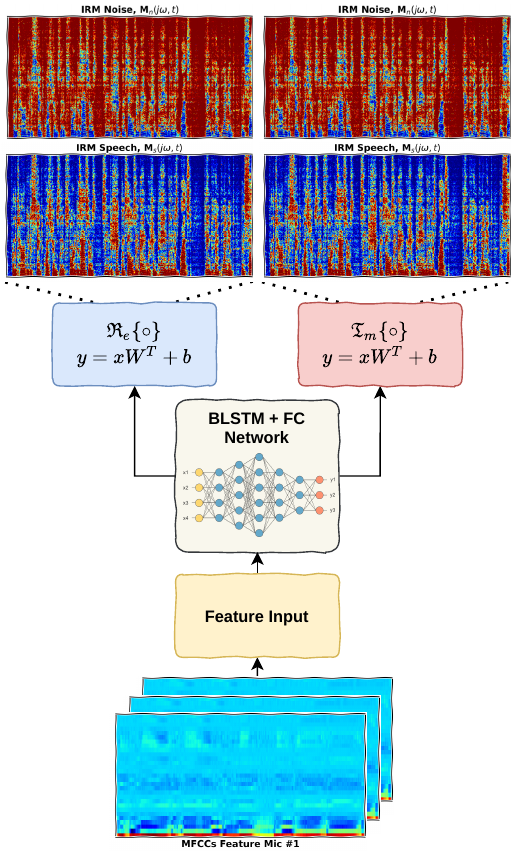
\includegraphics[width=0.75\linewidth]{Beamformers/images/cirm_nn}
    \caption{Proposed DNN for cIRM T-F masking estimations}\label{fig:cirm_nn}
\end{figure}


\begin{figure}[H]
    \centering
    \subfloat[\label{mel_fb_ref}]{%
       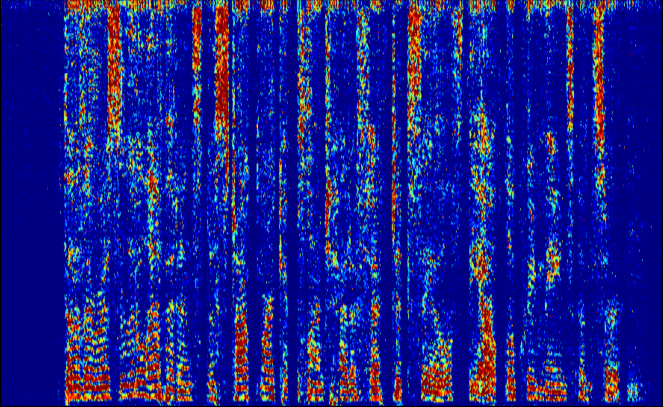
\includegraphics[width=0.45\linewidth]{Beamformers/images/cirm_r_s_ref}}
    \hspace{0.1cm}
    \subfloat[\label{mel_fbfcc_ref}]{%
        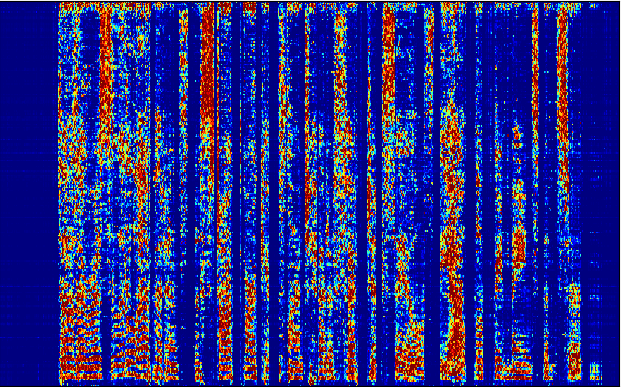
\includegraphics[width=0.444\linewidth]{Beamformers/images/cirm_r_s_nn}}
    \caption{(a) Reference cIRM
        real speech mask \(\mathbf{M}^{(s)}_{r}\);\;\;
        (b) The estimated cIRM
        real speech \(\mathbf{\widehat{M}}^{(s)}_{r}\).}\label{fig:cirm_nn_vs_ref} 
\end{figure}

Figure\;\ref{fig:cirm_nn_vs_ref} shows the reference real speech cIRM mask
compared to the estimated real speech mask predicted by the DNN model.
Looking at the figure, one can conclude that the model generalized correctly
as the estimated mask resembles the reference to a great extent.
Compared to the ``IRM'' DNN performance, the cIRM model 
with a compression in the range of \([-10, 10]\) performs better.

\subsection{Measurements}
Due to the complexity of the cIRM DNN model, 
it did not generalize properly for the evaluation dataset
with a number of epochs settings set to 50.
The results hence, are not accurate as a reference nor for comparison,
unless a retraining process is initialized with a sufficient number of epochs
to let the model generalize.

Due to the uncertainty of the impact the low number of epochs have
on the model performance, and the lack of time for a re-evaluation of the
DNN mask estimation, we decide to skip the results and 
to drop the cIRM measurements.

% \begin{figure}[H]
%     \centering
%     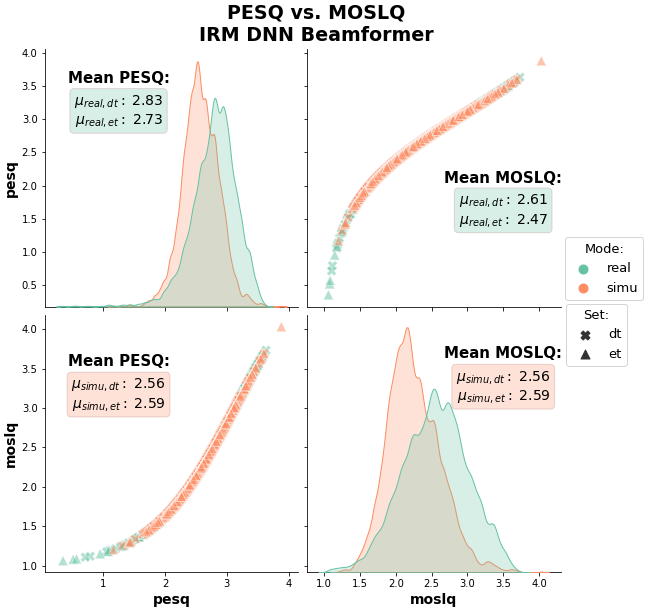
\includegraphics[width=\linewidth]{Experiments/images/irm_pesq_mosq}
%     \caption{IRM beamformer PESQ vs. MOSLQ}\label{fig:irm_pesq_mosq}
% \end{figure}

\section{PSM --- Phase Sensitive Mask}
The PSM T-F masking makes use of the magnitude ratios and phase differences
rather than requiring a complex multiplication.
In that way, the multiplication is taken in the real domain only,
while utilizing the phase contribution directly.

\begin{figure}[H]
    \centering
    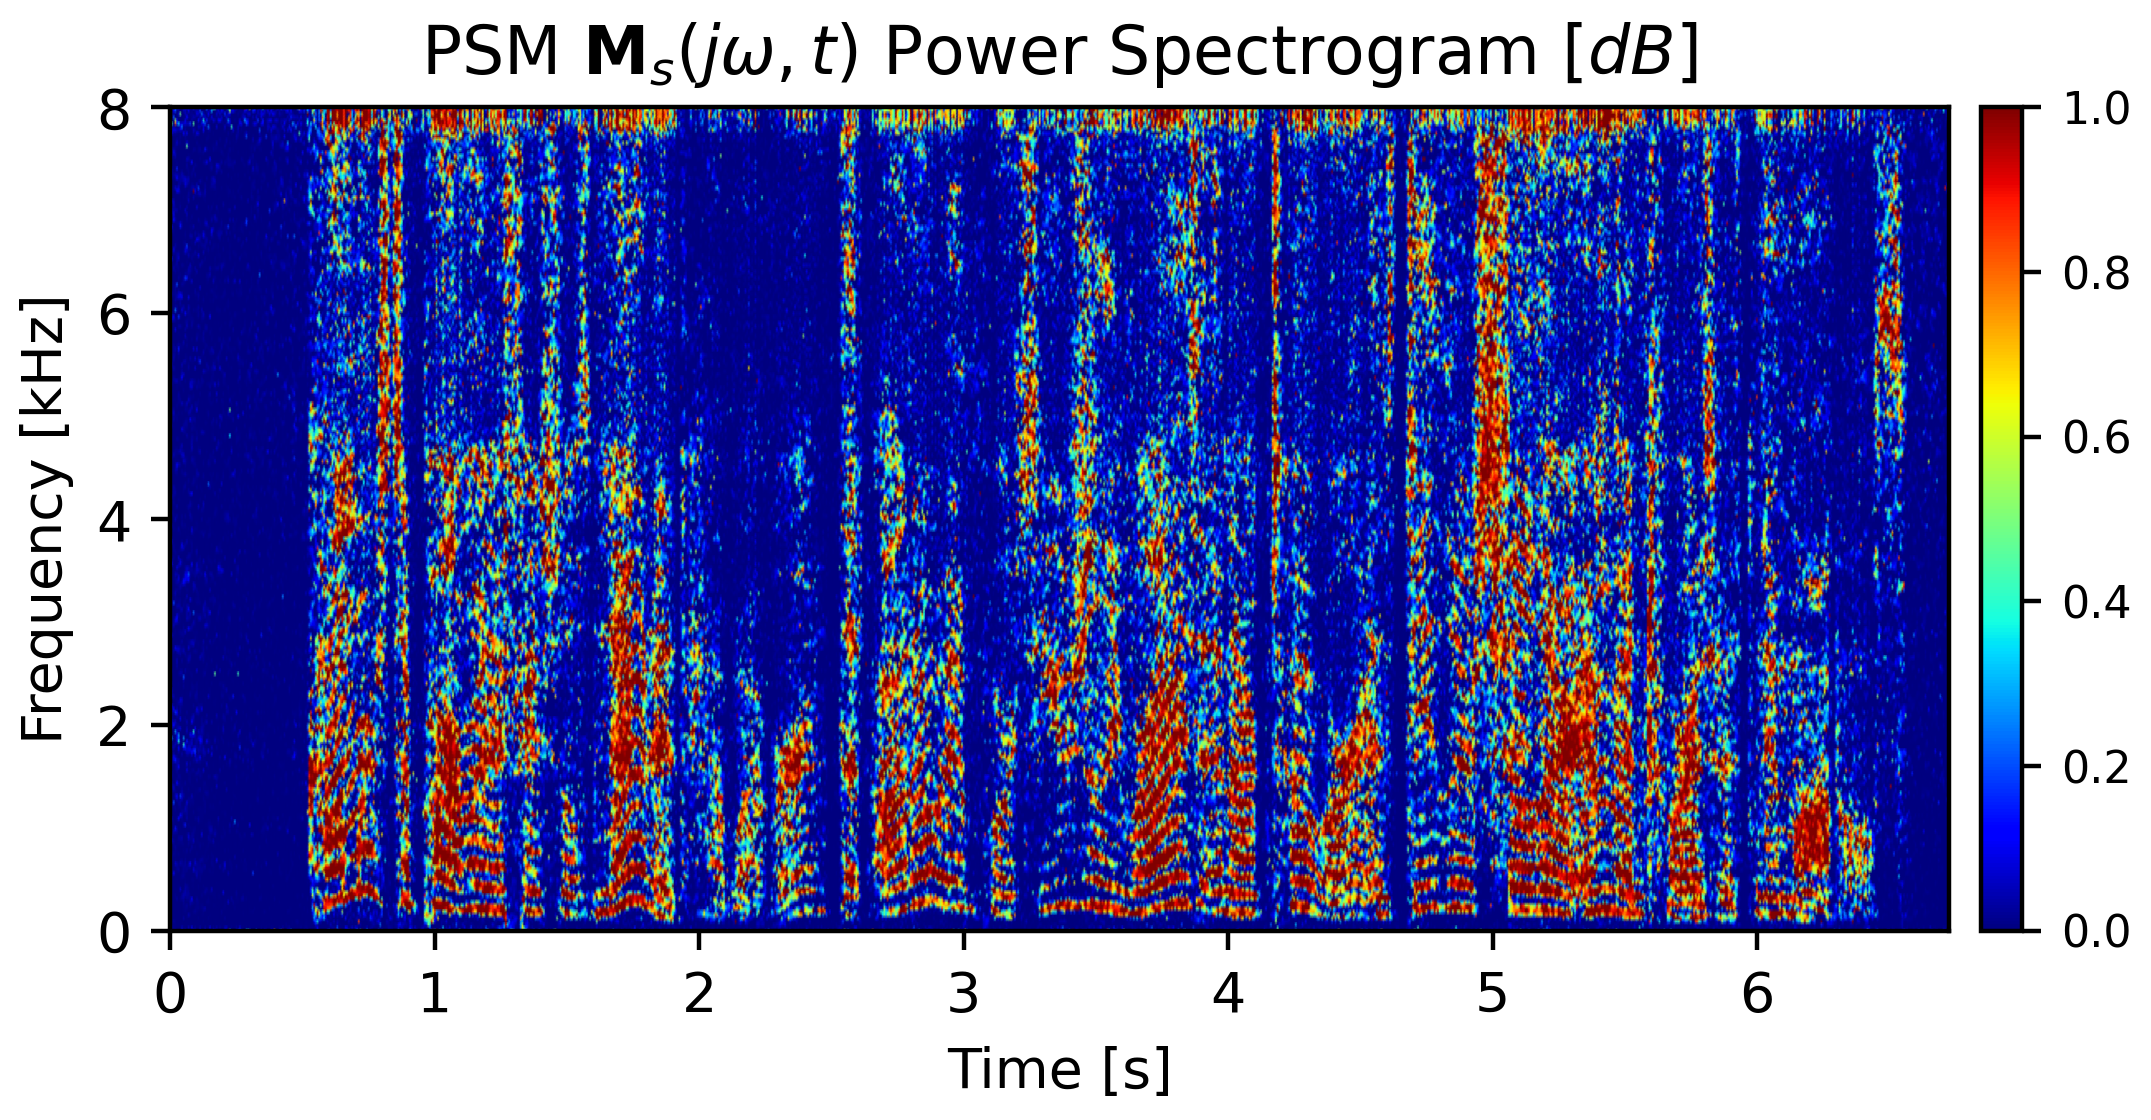
\includegraphics[width=\linewidth]{Features/images/psm_mask}
    \caption{PSM Speech Mask \(\mathbf{M}_{s}(j\omega, t)\)}\label{fig:psm_mask}
\end{figure}
\vspace{-0.5cm}
\begin{figure}[H]
    \centering
    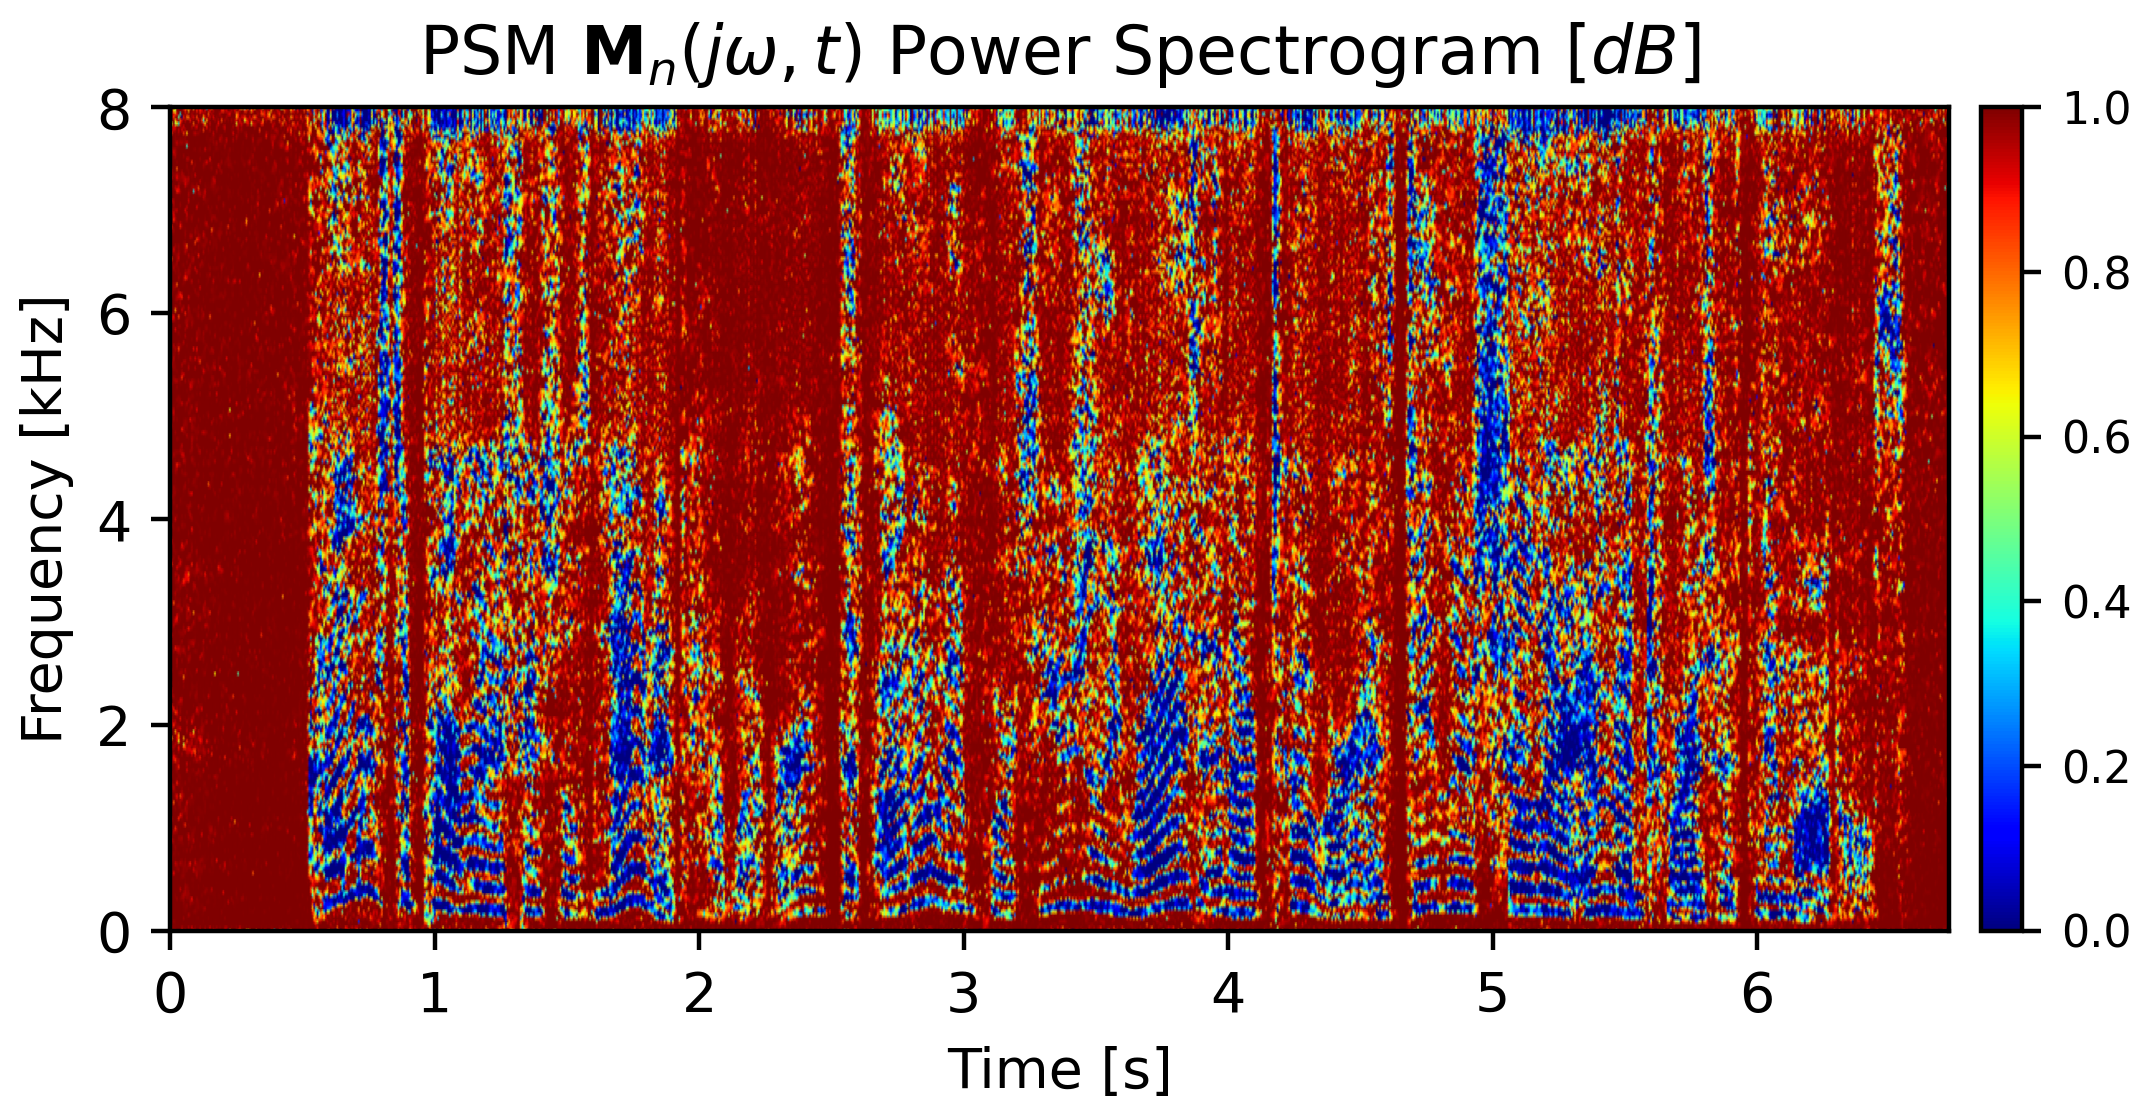
\includegraphics[width=\linewidth]{Features/images/psm_mask_noise}
    \caption{PSM Noise Mask \(\mathbf{M}_{n}(j\omega, t)\)}\label{fig:psm_mask_noise}
\end{figure}
The following equations give the PSM masks for the reference speech and noise,
\(\mathbf{M}^{(s)}_{j\omega, t}\) and \(\mathbf{M}^{(n)}_{j\omega, t}\):
\begin{align}
    \mathbf{M}^{(s)}_{j\omega, t} & = \frac{|\mathbf{S}(t,j\omega)|}{|\mathbf{Y}(t,j\omega)|} \cos(\bm{\theta}_{_{\mathbf{S}}} - \bm{\theta}_{_{\mathbf{Y}}}) \\
    \mathbf{M}^{(n)}_{j\omega, t} & = \frac{|\mathbf{N}(t,j\omega)|}{|\mathbf{Y}(t,j\omega)|} \cos(\bm{\theta}_{_{\mathbf{N}}} - \bm{\theta}_{_{\mathbf{Y}}})
\end{align}

\subsection{Masks Estimations}
Unlike the cIRM complex masks, the PSM masks are real valued.
However, the masks are not bounded similarly to the cIRM masks.
Therefore, the proposed model for the cIRM masks can be reused
with a slight difference in implementation. 
Now, only two outputs are created 
instead of branching to four outputs at the final layer.
One output for the speech mask and the other for the noise mask. 
The same as we did for the ``IRM'' but without the Sigmoids.
In addition, to deal with the unbounded range of values, 
we also apply apply a compression algorithm to the reference masks as well.
The compression mechanism is the same as 
described in Equation\;\ref{eq:cirm_compress}.

Following this architecture, the cost function can be set
to take two masks in the calculation of the error term,
like with the ``IRM'' masks:
\begin{align}\label{eq:psm_costf}
    \ell(\mathbf{\widehat{M}}_{j\omega, t},\;\mathbf{M}_{j\omega, t}) & = 
        \frac{1}{2N}\sum_{j\omega, t}
        \left[ 
            \beta\!\left( 
                \mathbf{\widehat{M}}^{(s)}_{j\omega, t} - 
                \mathbf{M}^{(s)}_{j\omega, t} 
            \right)^{2} 
            + \left( 1- \beta \right)\!
            \left(
                \mathbf{\widehat{M}}^{(n)}_{j\omega, t} - 
                \mathbf{M}^{(n)}_{j\omega, t} 
            \right)^{2} 
        \right]
\end{align}

The proposed PSM estimation network blocks diagram is shown in 
Figure\;\ref{fig:psm_nn}.

\begin{figure}[H]
    \centering
    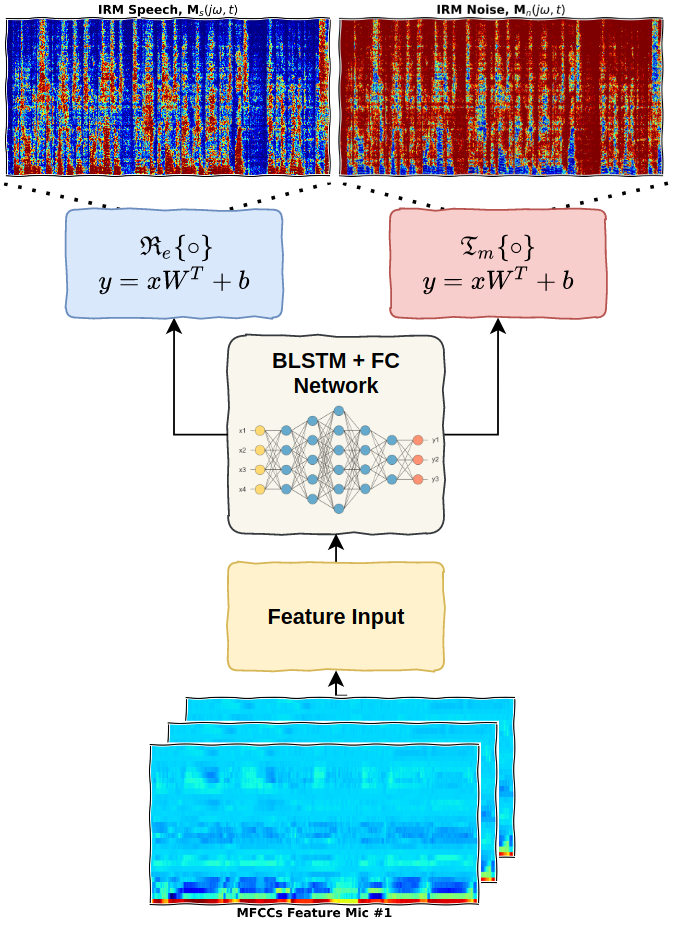
\includegraphics[width=0.75\linewidth]{Beamformers/images/psm_nn}
    \caption{Proposed DNN for PSM T-F masking estimations.}\label{fig:psm_nn}
\end{figure}

\subsection{Measurements}
\begin{figure}[H]
    \centering
    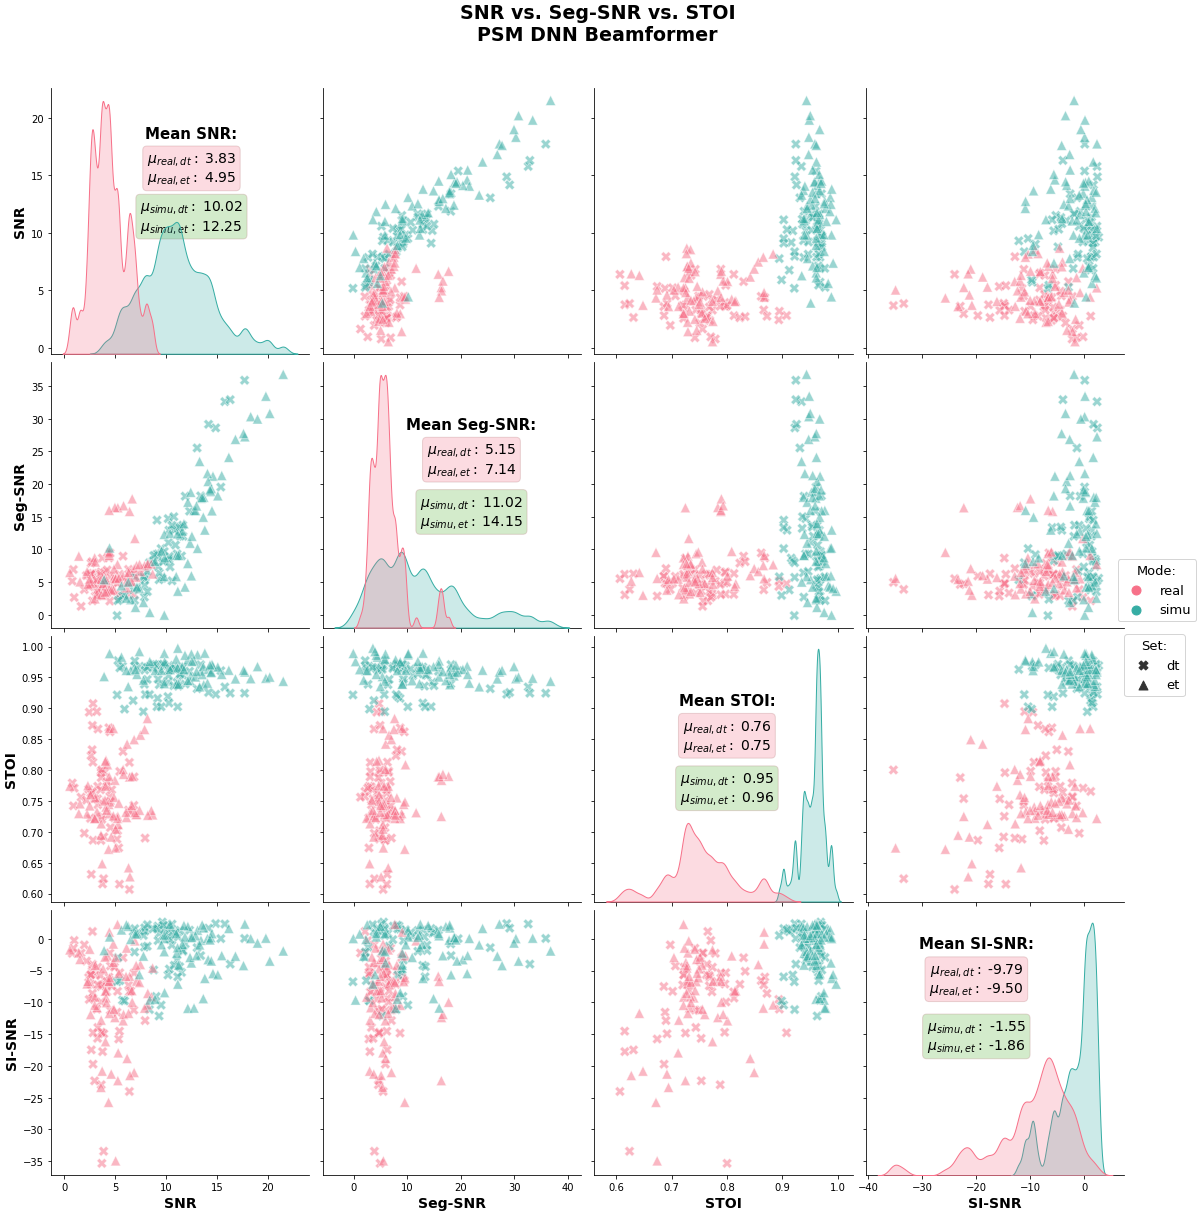
\includegraphics[width=\linewidth]{Features/images/psm_snr_stoi}
    \caption{PSM beamformer SNR vs. Segmental-SNR vs. STOI vs. SI-SNR.}\label{fig:psm_snr_stoi}
\end{figure}

\begin{figure}[H]
    \centering
    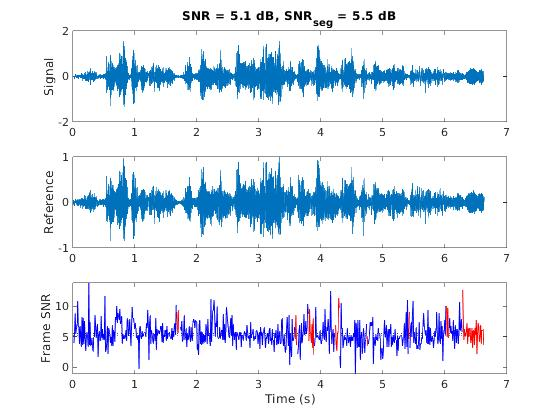
\includegraphics[width=\linewidth]{Features/images/psm_ideal_snr}
    \caption{Ideal PSM beamformer enhancement SNR \& Segmental-SNR.}\label{fig:psm_ideal_snr}
\end{figure}



\section{ORM --- Optimal Ratio Mask}
The realization of the phase component importance along with 
the desire to keep the masking as simple as possible in terms of number 
of matrices and the simplicity of multiplication for separation,
the IRM masking is further developed.

Trying to minimize the general MSE loss function for T-F masking,
same as with the ``Weiner filter'' that the IRM masking approximates, we get:
\begin{align}
    \mathbf{M}^{(s)}_{j\omega, t} & = \frac{
        |\mathbf{S}(t,j\omega)|^{2}
        + \mathfrak{R}_{e}\{ \mathbf{S}(t,j\omega) \cdot {\mathbf{N}}^{*}(t,j\omega) \}
        }{
            |\mathbf{S}(t,j\omega)|^{2} 
            + |\mathbf{N}(t,j\omega)|^{2}
            + 2 \mathfrak{R}_{e}\{ \mathbf{S}(t,j\omega) \cdot {\mathbf{N}}^{*}(t,j\omega) \} 
        } \\
    \mathbf{M}^{(n)}_{j\omega, t} & = \frac{
        |\mathbf{N}(t,j\omega)|^{2}
        + \mathfrak{R}_{e}\{ \mathbf{N}(t,j\omega) \cdot {\mathbf{S}}^{*}(t,j\omega) \}
        }{
            |\mathbf{S}(t,j\omega)|^{2} 
            + |\mathbf{N}(t,j\omega)|^{2}
            + 2 \mathfrak{R}_{e}\{ \mathbf{N}(t,j\omega) \cdot {\mathbf{S}}^{*}(t,j\omega) \} 
        }
\end{align}

Looking at the equation above, 
it resembles the IRM form but also introduces
the real part of the multiplication between the speech spectrum
and the conjugate noise spectrum.

\subsection{Masks Estimations}
The ORM masking in terms of the estimation process resembles the
PSM completely. Therefore, the same compression and 
DNN architecture are used to estimate the ORM masks.

The proposed DNN model blocks diagram is shown in Figure\;\ref{fig:psm_nn},
and the cost function is given in Equation\;\ref{eq:psm_costf}.

\subsection{Measurements}

\begin{figure}[H]
    \centering
    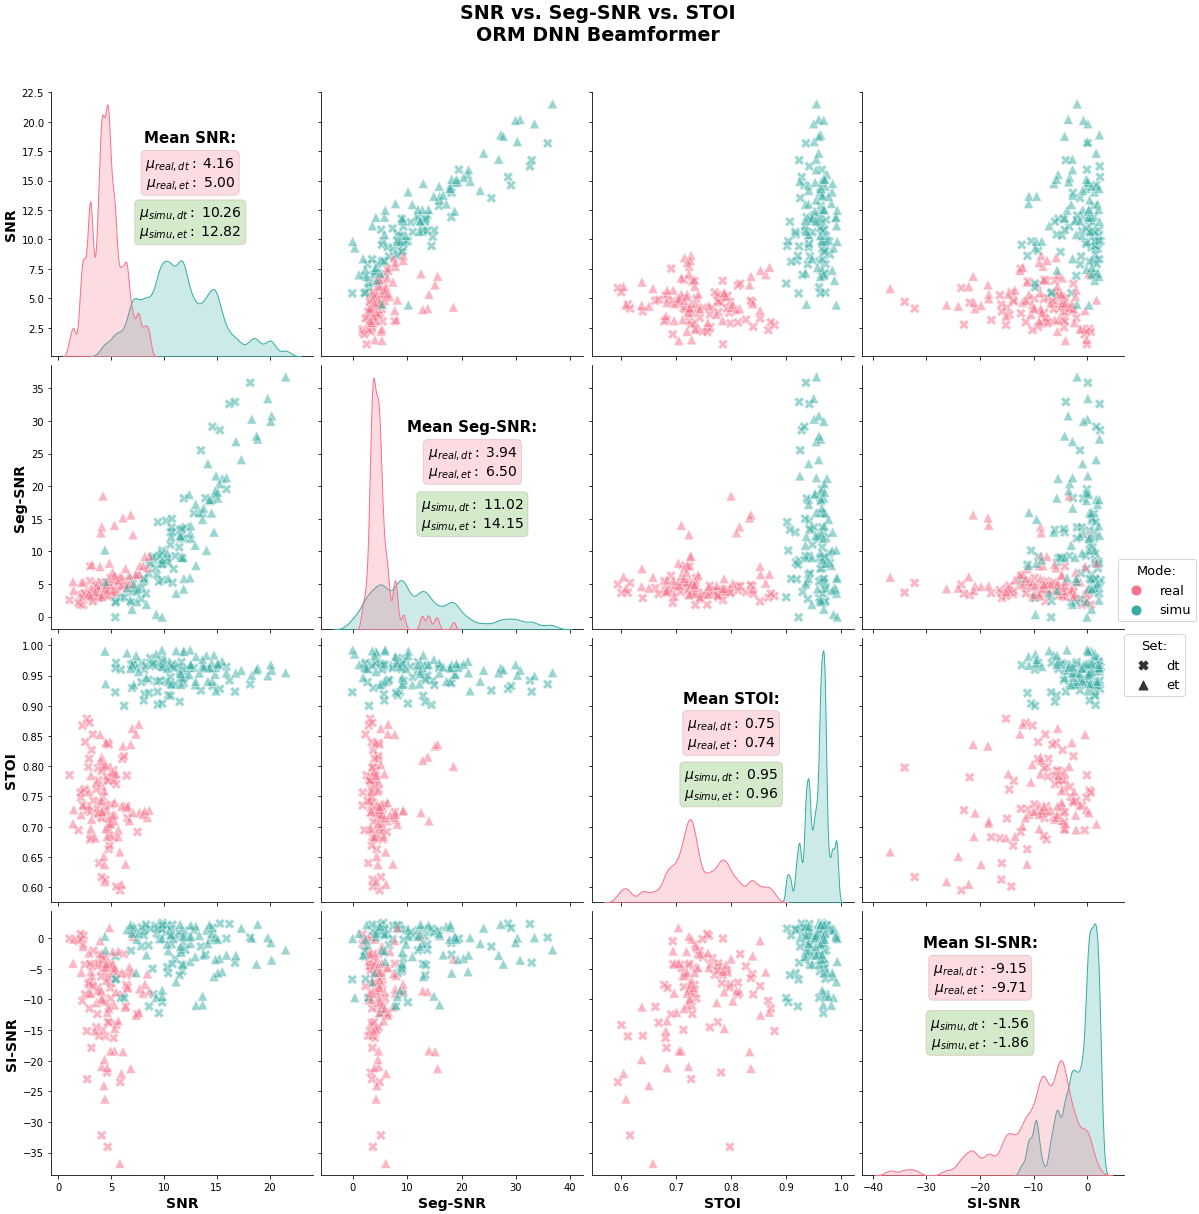
\includegraphics[width=\linewidth]{Features/images/orm_snr_stoi}
    \caption{ORM beamformer SNR vs. Segmental-SNR vs. STOI vs. SI-SNR.}\label{fig:orm_snr_stoi}
\end{figure}

\begin{figure}[H]
    \centering
    \includegraphics[width=\linewidth]{Features/images/orm_ideal_snr}
    \caption{Ideal ORM beamformer enhancement SNR \& Segmental-SNR.}\label{fig:orm_ideal_snr}
\end{figure}

% \section{Masks Estimations}
% \subsection{IRM}

% \begin{align}
%     \ell(\mathbf{\widehat{M}}_{j\omega, t},\;\mathbf{M}_{j\omega, t}) & = 
%         \frac{1}{2N}\sum_{j\omega, t}
%         \left[ 
%             \beta\!\left( 
%                 \mathbf{\widehat{M}}^{(s)}_{j\omega, t} - 
%                 \mathbf{M}^{(s)}_{j\omega, t} 
%             \right)^{2} 
%             + \left( 1- \beta \right)\!
%             \left(
%                 \mathbf{\widehat{M}}^{(n)}_{j\omega, t} - 
%                 \mathbf{M}^{(n)}_{j\omega, t} 
%             \right)^{2} 
%         \right]
% \end{align}

% \begin{figure}[H]
%     \centering
%     \includegraphics[width=0.75\linewidth]{Beamformers/images/irm_nn}
%     \caption{Proposed DNN for IRM T-F masking estimations}\label{fig:irm_nn}
% \end{figure}

% \subsection{cIRM}
% In Section~\ref{ssec:cirm}, 
% the \(cIRM\) masks are described in 
% Equations~\ref{eq:cirmr_mask},~\ref{eq:cirmi_mask}.
% In contrast to the \(IRM\) masks which are bounded in the range \([0, 1]\),
% the \(cIRM\) masks are unbounded, and have the range \((-\infty, \infty)\).

% A neural network cannot train for unbounded values. 
% Hence, an alternative presentation to the mask values is needed.
% One possibility is to compress the real and imaginary masks
% with a hyperbolic tangent as suggested in \cite{}: 
% \begin{align}
%     cIRM_{x} &= K \frac{1-e^{-C\cdot M_{x}}}{1+e^{-C\cdot M_{x}}}
% \end{align}

% Where \(x\), stands for the real or the imaginary parts of the mask.
% By applying this compression, the mask values are bounded in
% the range \([-K, K]\), while \(C\) controls the steepness.
% In that way, a linear layer at the output is placed
% in favor of the sigmoid layers used in the simpler IRM DNN.

% Then, the cost function is defined to include both real and imaginary parts
% of both the noise and speech masks. 
% \begin{align}
%     \ell(\mathbf{\widehat{M}}^{(x)}_{j\omega, t},\;\mathbf{M}^{(x)}_{j\omega, t}) & = 
%         \frac{1}{2N}\sum_{j\omega, t}
%         \left[ 
%             \beta\!\left( 
%                 \mathbf{\widehat{M}}^{(s \in \mathbb{C})}_{j\omega, t} - 
%                 \mathbf{M}^{(s \in \mathbb{C})}_{j\omega, t} 
%             \right)^{2} 
%             + \left( 1- \beta \right)\!
%             \left(
%                 \mathbf{\widehat{M}}^{(n \in \mathbb{C})}_{j\omega, t} - 
%                 \mathbf{M}^{(n \in \mathbb{C})}_{j\omega, t} 
%             \right)^{2} 
%         \right]
% \end{align}

% \begin{figure}[H]
%     \centering
%     \includegraphics[width=0.75\linewidth]{Beamformers/images/cirm_nn}
%     \caption{Proposed DNN for cIRM T-F masking estimations}\label{fig:cirm_nn}
% \end{figure}


% \subsection{PSM}

% \subsection{ORM}

\section{Conclusions}
In Table\;\ref{tbl:masks_l_params} are presented
the model's sizes in terms of memory requirement
and the number of learnable parameters.
The model's parameters were quantized
to the form of signed 16 bits. 
The MSB (most significant bit) is for the sign,
the following four bits are set for the integer part,
and the other eleven bits present the fractional part.
All of the tested models were trained with and without
the \(\Delta, \Delta\Delta\) features.
Usage of the additional \(\Delta, \Delta\Delta\) features
enlarges the input size of the model and thus
leading to a larger number of learnable parameters, resulting
in a bigger model. Bigger models take a longer time to train
and are more complex to fit in limited resources hardware 
devices. A trade-off decision can be made with respect to
the memory size and desired performance in the design phase
of T-F masks based applications. Although presenting
better results in audio metrics, the PSM and ORM
masks require \(\sim 43\%\) larger memory space
compared to the IRM masks, 
when the feature set does not include
the \(\Delta, \Delta\Delta\) features.
A less severe increase of \(\sim 22\%\) in memory 
size requirement has been observed 
when the \(\Delta, \Delta\Delta\) features
were not excluded from the feature set.




\begin{table}[H]
    % for more info see: https://www.overleaf.com/learn/latex/tables
    \centering
    % \hspace*{-2.8cm}
    \arrayrulecolor{mtblborder}
\begin{tabular}{ !{\color{mtblborder}\vrule}c!{\color{mtblborder}\vrule}cc|||cc| } 
    \hline

    \hline
    \rowcolor{mtblcaption}
    & \multicolumn{2}{c}{\color{white}\bf{Learnable Parameters} [Mil]}
    & \multicolumn{2}{c}{\color{white}\bf{Quant. (S16.11) Mem } [Mb]}\\         
    % \cline{2-8}
    
    \multirow{-2}{*}{\cellcolor{mtblcaption}\color{white}\bf{Targets} }
    & \cellcolor{mtbl} \color{black}{W/o (\(\Delta\),\(\Delta\Delta\))} 
    & \cellcolor{mtbl} \color{black}{W/ (\(\Delta\),\(\Delta\Delta\))}
    & \cellcolor{mtbl} \color{black}{W/o (\(\Delta\),\(\Delta\Delta\))} 
    & \cellcolor{mtbl} \color{black}{W/ (\(\Delta\),\(\Delta\Delta\))} \\
    % & \color{white}\bf{ORM} 
    % & \color{white}\bf{Clean} \\
    \hline

    \hline
    \rowcolor{mtblA} IRM  
        & 2.44 
        & 4.67
        & 39.0
        & 74.8 \\
    \hline
    
    \hline
    \rowcolor{mtbl} cIRM  
        & 3.76
        & 5.99
        & 60.1
        & 95.9 \\
    \hline

    \hline
    \rowcolor{mtblA} PSM  
        & 3.49
        & 5.73
        & 55.9
        & 91.7 \\
    \hline

    \hline
    \rowcolor{mtbl} ORM  
        & 3.50
        & 5.74
        & 56.0
        & 91.8 \\
    \hline
    
    \hline
\end{tabular}
\arrayrulecolor{black}
\caption{T-F Masks models learnable parameters vs. Required memory size}
\label{tbl:masks_l_params}
\end{table}
  \cleardoublepage
  \printbibliography[title={References}]
\end{refsection}

\begin{refsection}[Beamformers/beamformers.bib]
  \chapter{Beamformers}
\section{Types}

\subsection{MVDR}
\subsection{GEV}
\subsection{Sum-and-Delay}

\section{Static Coefficients}

\section{Dynamic Coefficients}
\subsection{DNN Estimations}
\section{Masks Estimations}
  \cleardoublepage
  \printbibliography[title={References}]
\end{refsection}


\begin{refsection}[ASR/asr.bib]
  \chapter{ASR -- Automatic Speech Recognition}\label{ch:asr_ch}
\section{Introduction}
Speech recognition (SR) stands for recognizing 
natural speech and translating 
it to readable text named transcript.
Often speech recognition is referred to as Speech-to-Text (STT). 
Speech recognition 
that is accomplished 
automatically by a computing machine or 
software is known as ASR (Automatic Speech Recognition).

ASR systems employ numerous algorithms 
and techniques to conduct the speech to text translation.
Some algorithms aim for precision improvements
and higher detection ratios measured with \emph{WER},
\emph{CER}
and \emph{PER},
as described in Chapter\;\ref{ch:features}.
Other algorithms target increasing
the system's robustness, which means
how well the system can still function adequately
given that the environmental conditions
are not static and change.

Naturally spoken speech has inherent 
variabilities depending on many 
factors that make a speech signal 
classified as non-stationary and inconsistent. 
Natural speech heavily depends on the speaker's gender, 
whether a male or a female, and the speaker's age. 
Moreover, different speakers of the same 
gender and age range may still present variances 
in the vocal range, pitch, and formant frequencies.
Likewise, we can say that gender-independent 
characteristics such as accent, style of speech, emotional state, 
or health conditions, 
which are examples of social and geographical factors, 
all impact naturally spoken sentences and 
introduce some degree of variability.

Due to the high dependency that natural speech has on so many factors, 
an ASR system must have high endurance to fluctuations in these 
previously mentioned environments and states. Also, the ability to perform adequately in a wide range of scenarios is very crucial.  
In particular, the cases of high background noise levels in low SNR scenarios and multiple reverberations due to poor room acoustics.

Traditional ASR engines 
are usually built of several 
modules designated for a specific task.
An ASR engine as a whole is a chain of these modules connected in a pipeline. 
A common structure of an ASR system
is shown in Figure\;\ref{fig:asr_blocks}. This type
of ASR system translates a speech waveform into a transcript
by chaining \emph{phonemes} together to construct words.

A phoneme is a discrete and distinctive unit of language
that can be used to differentiate between words.
A word is a sequence of phonemes chained together in how the word is 
actually pronounced. 
The motivation of detecting phonemes instead of entire words by the ASR engine relies on the fact that the number of words in a common language crosses the tens of thousands and sometimes even larger than hundreds of thousands. 
Extensive word vocabulary implies a huge training dataset 
requirement covering most of the words in a selected language.
On the contrary, most languages have 20-60 phonemes\cite{Blust2013TerrorFT, dixon_1997}.
In that way, a much smaller set of dedicated phonemes can be used to construct the vocabulary utilizing a less demanding training dataset requirement.

\begin{figure}[H]
    \centering
    \subfloat[\label{fig:asr_blocks}]{%
       \includegraphics[width=0.75\linewidth]{ASR/images/asr_blocks}}
    \\
    \subfloat[\label{fig:e2e_asr_blocks}]{%
        \includegraphics[width=0.75\linewidth]{ASR/images/e2e_asr_blocks}}
    \caption{(a) Traditional ASR system blocks diagram;\;\;
        (b) End-to-end ASR system blocks diagram.}\label{fig:tr_e2e_asr_blocks} 
\end{figure}

The system presented in Figure\;\ref{fig:asr_blocks} 
shows a pipeline that starts with a pre-emphasis and features
extraction modules. 
The pre-emphasis includes the speech analysis, noise cancellation, speech enhancements, windowing, and framing of the speech into sub-frames in which it is closer in characteristics to a stationary signal.
The feature extraction module extracts the individual 
features representing the speech from the incoming frames 
as MFCCs, FilterBanks, and other techniques.

The next module in line is the decoder. The decoder's responsibility is to take the features, convert them to a set of phonemes and chain them together to detectable words, composing the transcript at the output.
A decoder is built from three sub-models tied
together that work in harmony. 
The first is the Acoustic Model (AM), which maps the acoustic features extracted in the earlier module to phoneme sequences with probabilistic weights.
These phonemes are an intermediate representation in the process of word decoding.
An additional module is the pronunciation model. This module is a dictionary, handcrafted by an expert linguist and tailor-made to each language explicitly.
This dictionary links phoneme sequences
to words. 
Lastly, the Language Model (LM) calculates the likelihood a given word is detected based on the perceived phoneme sequences and how likely it is for this word to occur given the past temporal context.
The words or N-Grams with the highest scores are selected and written into the output transcript.

A newer more modernized approach known as 
End-to-End Automatic Speech
Recognition (E2E ASR) has been proposed 
in \cite{pmlr-v32-graves14}. This approach 
replaces the conventional decoder structure with 
a deep neural network of some kind that maps 
acoustic features to characters. An E2E ASR system
structure is presented in Figure\;\ref{fig:e2e_asr_blocks}.

With this architecture, there is no longer a need for expert 
dictionaries or complex models of chaining phonemes to words.
That spares the need to acquire new pronunciation models or maintain an existing one, which can be expensive. 
Instead, character probabilities 
are given at the output according to the learning
process of mapping acoustic features to 
corresponding letters.
That leads to another advantage of E2E ASR systems
over traditional ASRs. 
Retraining an E2E model with 
a new dataset of annotated speech in different 
languages is possible without changing the architecture at all.
On the other hand, 
using E2E systems means a more extensive training dataset is 
required for the model to generalize well, 
only to maintain comparable detection 
ratios in terms of WER and CER as the traditional ASRs do.

However, despite having an E2E system trained against a huge dataset, the direct estimations of characters and, later on, the construction of a full 
transcript don't work as expected compared to traditional ASRs.
To overcome the degradation in performance, several algorithms
can be applied to improve different aspects of the model.
Such a helpful technique that is 
called CTC (Connectionist Temporal Classification) 
by Maas et al. is presented \cite{maas-etal-2015-lexicon}.
For example, this method demonstrates which characters get the highest 
probability for specific phonemes, 
as shown in
Figure\;\ref{fig:CTC_maas_graph}. 
% Therefore, a more accurate selection of 
% letters is achievable by utilizing a \emph{beam-search}.

\begin{figure}[H]
    \centering
    \includegraphics[width=0.95\linewidth]{ASR/images/CTC_maas_graph}
    \caption{Maas et al. \cite{maas-etal-2015-lexicon} phonemes vs characters graphs}\label{fig:CTC_maas_graph}
\end{figure}

Additional paradigm by Chan et al. known as Seq2Seq (Sequence-to-Sequence) or sometimes as Attention Encoder-Decoder (AED) networks
is presented in \cite{44926}.
This approach is based on an LSTM transducer.
A more advanced model that is known for its self-attention mechanism 
was later suggested by Vasawani et al. in 2017 \cite{vaswani2017attention}.
This model, which also uses the Encoder-Decoder architecture, is called a transformer.

A sophisticated combination of these techniques is practically used in this work to construct and evaluate the different tested ASR engines.

% \begin{figure}[H]
%     \centering
%     \includegraphics[width=0.75\linewidth]{ASR/images/asr_blocks}
%     \caption{Traditional ASR system blocks diagram}\label{fig:asr_blocks}
% \end{figure}

% \begin{figure}[H]
%     \centering
%     \includegraphics[width=0.75\linewidth]{ASR/images/asr_blocks}
%     \caption{End-to-end ASR system blocks diagram}\label{fig:asr_blocks}
% \end{figure}

\section{The ASR Engine}
The proposed general architecture for the suggested 
ASR engines listed in Table\;\ref{tbl:asr_engines} 
is constructed with a CNN front-end connected to
a self-attention based transformer, 
implying an Encoder-Decoder infrastructure. 

% Joint CTC (Connectionist Temporal Classification) + Seq2Seq (Sequence-To-Sequence) Transformer (self-attention) based.

\subsection{Front-End}
\begin{figure}[H]
    \centering
    \includegraphics[width=0.45\linewidth]{ASR/images/single_convblock}
    \caption{CNN front-end general ConvBlock architecture.}\label{fig:transformer_cnn_convblock}
    % \source{Adapted from \citep{ADI_MIMO}}
\end{figure}

\subsection{Transformer}
A transformer is a self-attention Encoder-Decoder
based model whose architecture is
shown in Figure\;\ref{fig:transformer_blocks}.
The left side is the Encoder, and the right
side is the Decoder.

\begin{figure}[H]
    \centering
    \includegraphics[width=0.75\linewidth]{ASR/images/transformer_blocks}
    \caption{Transformer}\label{fig:transformer_blocks}
    \source{Adapted from ``Attention Is All You Need'' \cite{vaswani2017attention}}
\end{figure}

The attention function that translates 
the Query \((Q)\) and the keys-values pairs \((K)\), \((V)\),
respectively, can be implemented in Scaled Dot-Product Attention
or in Multi-Head Attention.
The transformer backend used in this work is
a Multi-Head Attention-based utilizing
eight heads in the attention model. The Encoder 
and Decoder parts consist of a variable
number of linear layers ranging from four to eight.
The activation function used
with the transformer is the \emph{GELU} (Gaussian
Error Linear Unit).

\subsection{CTC}
The CTC loss is the negative logarithm of the probabilities that resulted
from the CTC algorithm. Minimizing the CTC loss is in fact selecting
the characters that end up with the highest probabilities. 
As a result, the predicted label collapses, 
meaning that any repeated characters not separated by the 
``blank'' character unite into a single character.

\begin{equation}
    \hat{\theta} = arg \min_{\theta} - \sum_{i=1}^{N} \left[ \sum p\left( \pi | x^{(i)}; \theta \right) \right]
\end{equation}

\subsection{Seq2Seq}
\begin{equation}
    \ell(x, y) = L = \left\{ \ell_{_{1}}, \ell_{_{2}}, ..., \ell_{_{N}} \right\} 
\end{equation}
\begin{equation}
    \ell_{_{n}} = y_{_{n}} \left[ \log \left( y_{_{n}} \right) - x_{_{n}} \right]
\end{equation}
The kldiv loss also can be reduced over the mini-batch size, as follows:
\begin{equation}
    \ell(x, y) = \begin{cases}
        \frac{\sum {L}}{batch\_size}, & red=meanbatch \\
        \sum {L}, & red=sum
    \end{cases}
\end{equation}
Combining both the CTC and the Seq2Seq components,
the engine's loss function used for training is as follows:
\begin{equation}
    \ell = \omega_{_{ctc}}  \ell_{_{ctc}} + (1 - \omega_{_{ctc}}) \cdot \ell_{_{seq}}
\end{equation}
Where \(\omega_{_{ctc}}\) is set to 0.3 and a greater weight of 0.7 is
given to the Seq2Seq loss \(\ell_{_{seq}}\).

% Feature Extraction:
% N FFT = 400
% N Filters (Mels) = 80

% \subsection{Training Process}
% Batch: 5
% num samples = 150000


% \subsection{FB Feature}
% CNN :
% input shape: (8, 10, 80)
% num blocks: 3
% num layers per block: 1
% out channels: (128, 200, 256)
% kernel sizes: (3, 3, 1)
% strides: (2, 2, 1)
% residuals: (False, False, False)

% Transformer input size = 80 / 2(Cnn1) / 2(Cnn2) · 256
%                             = 20 · 256 = 5120
                            
% \subsection{MFCC + deltas Features}
% Transformer input size = 60 / 2(Cnn1) / 2(Cnn2) · 256
%                             = 15 · 256 = 3840

% \subsection{Validation Process}

% \subsection{Testing Process}

% Transformer Encoder
% Transformer Decoder + (CTC/ATT joint) beamsearch

% Tokens: unigram 500



% \subsection{RNN Based Transducer}

% \subsection{AED CTC Seq2Seq}

\begin{table}[H]
    % for more info see: https://www.overleaf.com/learn/latex/tables
    % \centering
    \hspace*{-2.8cm}
    \arrayrulecolor{ytblborder}
\begin{tabular}{ !{\color{ytblborder}\vrule}l!{\color{ytblborder}\vrule}lrllrr| } 
    \hline

    \hline
    \rowcolor{ytblcaption} \color{white}\bf{Id(seed)} 
    & \color{white}\bf{Feature(s)} 
    & \color{white}\bf{Params} 
    & \color{white}\bf{Scale} 
    & \color{white}\bf{Fbank} 
    & \color{white}\bf{\#Filt.} 
    & \color{white}\bf{\#Coeff.} \\
    % & \color{white}\bf{ORM} 
    % & \color{white}\bf{Clean} \\
    \hline

    \hline\hline
    \rowcolor{wtbl}\multicolumn{7}{|c|}{\bf{Root Mean Cepstral Coefficients}}   \\
    \hline

    \hline
    \rowcolor{ytbl}  \#1(5)  
        & RMFCC(0.1), \(\Delta\), \(\Delta\Delta\) 
        & 146.2M
        & Mel 
        & Bartlett
        & 80 
        & 20 \\
    \hline
    
    \hline
    \rowcolor{wtbl}  \#2(15)  
        & RMFCC(0.08), \(\Delta\), \(\Delta\Delta\) 
        & 146.2M
        & Mel 
        & Bartlett
        & 80 
        & 20 \\
    \hline
    
    \hline
    \rowcolor{ytbl}  \#3(12)  
        & RBFCC(0.1), \(\Delta\), \(\Delta\Delta\) 
        & 146.0M
        & Bark 
        & Bartlett
        & 28 
        & 18 \\
    \hline

    \hline
    \rowcolor{wtbl}  \#4(13)  
        & RGFCC(0.1), \(\Delta\), \(\Delta\Delta\) 
        & 146.0M
        & ERB
        & Gammatone
        & 28 
        & 18 \\
    \hline

    \hline\hline
    \rowcolor{wtbl}\multicolumn{7}{|c|}{\bf{Conventional Cepstral Coefficients}}   \\
    \hline

    \hline
    \rowcolor{ytbl}  \#5(70)  
        & MFCC, \(\Delta\), \(\Delta\Delta\) 
        & 146.2M
        & Mel 
        & Bartlett
        & 80 
        & 20 \\
    \hline
    
    \hline
    \rowcolor{wtbl}  \#6(72)  
        & MFCC, \(\Delta\), \(\Delta\Delta\) 
        & 146.0M
        & Mel 
        & Bartlett
        & 28 
        & 18 \\
    \hline

    \hline
    \rowcolor{ytbl}  \#7(22)  
        & MFCC, \(\Delta\), \(\Delta\Delta\) 
        & 146.0M
        & Bark 
        & Bartlett
        & 28 
        & 18 \\
    \hline

    \hline
    \rowcolor{wtbl}  \#8(23)  
        & MFCC, \(\Delta\), \(\Delta\Delta\) 
        & 146.0M
        & ERB
        & Gammatone
        & 28 
        & 18 \\
    \hline

    \hline
    \rowcolor{ytbl}  \#9(100)  
        & MFCC, \(\Delta\), \(\Delta\Delta\), Context(3, 3)
        & 78.8M
        & Mel 
        & Bartlett
        & 26 
        & 26 \\
    \hline

    \hline
    \rowcolor{wtbl}  \#10(101)
        & MFCC, \(\Delta\), \(\Delta\Delta\), Context(3, 3)
        & 78.8M
        & Mel Approx.
        & Bartlett
        & 26 
        & 26 \\
    \hline

    \hline
\end{tabular}
\arrayrulecolor{black}
\caption{ASR Engines Table}
\label{tbl:asr_engines}
\end{table}
\vspace{-0.7cm}
ASR engines \#9, \#10 were heavily 
optimized in terms of the neural network structures, 
leading to smaller models having two times fewer learnable parameters.
For comparison, differences between ASR engines 101
and 72 are summarized in
Table\;\ref{tbl:engine_101_72}.
\begin{table}[H]
    % for more info see: https://www.overleaf.com/learn/latex/tables
    \centering
    % \hspace*{-2.8cm}
    \arrayrulecolor{ytblborder}
\begin{tabular}{ !{\color{ytblborder}\vrule}l!{\color{ytblborder}\vrule}cc| } 
    \hline

    \hline
    \rowcolor{ytblcaption} \color{white}\bf{Parameter} 
    & \color{white}\bf{Engine \#10} 
    & \color{white}\bf{Engine \#6} \\
    % & \color{white}\bf{ORM} 
    % & \color{white}\bf{Clean} \\
    \hline

    \hline\hline
    \rowcolor{wtbl}\multicolumn{3}{|c|}{\bf{CNN Settings}}   \\
    \hline

    \hline
    \rowcolor{ytbl}  CNN Blocks [\#]  
        & 3 
        & 3 \\
    \hline
    
    \hline
    \rowcolor{wtbl}  CNN Shapes  
        & [64, 100, 128]
        & [128, 200, 256] \\
    \hline

    \hline\hline
    \rowcolor{wtbl}\multicolumn{3}{|c|}{\bf{Transformer Settings}}   \\
    \hline

    \hline
    \rowcolor{ytbl}  FFN layers  
        & 2048
        & 3072 \\
    \hline

    \hline
    \rowcolor{wtbl}  Input size
        & 2560
        & 3584 \\
    \hline

    \hline
    \rowcolor{ytbl}  Enc. layers
        & 8
        & 12 \\
    \hline

    \hline
    \rowcolor{wtbl}  Dec. layers
        & 4
        & 6 \\
    \hline


    \hline\hline
    \rowcolor{wtbl}\multicolumn{3}{|c|}{\bf{Implementation Settings}}   \\
    \hline

    \hline
    \rowcolor{ytbl}  Filters [\#] 
        & 26
        & 28 \\
    \hline

    \hline
    \rowcolor{wtbl} Coeff. [\#]  
        & 2048
        & 3072 \\
    \hline

    \hline
    \rowcolor{ytbl} Precision  
        & U16/8
        & FP64 \\
    \hline

    \hline
\end{tabular}
\arrayrulecolor{black}
\caption{ASR engines \#10, \#6 comparison table}
\label{tbl:engine_101_72}
\end{table}


% \begin{figure}[H]
%     \centering
%     \includegraphics[width=0.75\linewidth]{Experiments/images/asr_5}
%     \caption{ASR \#1 training }\label{fig:asr_5}
% \end{figure}

% \begin{figure}[H]
%     \centering
%     \includegraphics[width=0.75\linewidth]{ASR/images/asr5_wer.png}
%     \caption{ASR \#1 WER, CER results}\label{fig:asr5_wer}
% \end{figure}

\subsection{Trained Engines}
\subsubsection{ASR Engine \#1 -- RFCC(0.1), \(\Delta,\;\Delta\Delta\)}
ASR engine \#1 had been trained over fifteen epochs,
against a \(400K\) recordings table, with a minibatch size 
of four per iteration. 
The engine was trained against the RFCCs, 
when \(\gamma=0.1\),
with the \(\Delta,\;\Delta\Delta\) features, utilizing
the Log-Mel scale. A preprocessing STFT enframing
block was set with
80 Bartlett filters for each T-F bin.
Overall the number of features
per T-F unit is 20 cepstral coefficients plus the
first and second derivatives.
Figure\;\ref{fig:asr_5} shows ASR engine \#1 training results
for the test and validation subsets.
In Figure\;\ref{fig:asr5_wer},
we present the evaluated WER and CER measures
taken every five epochs during the training process.

\begin{figure}[H]
    \centering
    \subfloat[\label{fig:asr_5}]{%
       \includegraphics[width=0.85\linewidth]{Experiments/images/asr_5}}
    \\
    \vspace{-0.3cm}
    \subfloat[\label{fig:asr5_wer}]{%
        \includegraphics[width=0.85\linewidth]{ASR/images/asr5_wer}}
    \caption{(a) ASR \#1 training accuracy and loss plot;\;\;
        (b) ASR \#1 WER, CER evaluation plot.}\label{fig:asr5_wer_subplot} 
\end{figure}

\begin{figure}[H]
    \centering
    \includegraphics[width=0.95\linewidth]{ASR/images/asr5_wer_masks.png}
    \caption{ASR \#1 WER, CER vs. T-F masks, noisy and clean inputs}\label{fig:asr5_wer_masks}
\end{figure}

In Figure\;\ref{fig:asr5_wer_masks}, we present the engine's
results in terms of WER and CER per each subset of
the multi microphone CHiME dataset.
This figure emphasizes the comparison between the
four T-F masking algorithms. Results are plotted side by side with
the evaluated noisy mixture and clean speech metrics as reference.
Two horizontal lines, red and blue, are stretched across the x-axis
of each plot. These lines mark the plot's metric, 
whether WER or CER, taken from the training evaluations of 
CommonVoice datasets validation and test subsets.
The red line is for the test measurement
and the blue line marks the validation measurement.

\subsubsection{ASR Engine \#2 -- RMFCC(0.08), \(\Delta,\;\Delta\Delta\)}
ASR engine \#2 had been trained over fifteen epochs,
along a \(400K\) recordings table, with a minibatch size 
of four per iteration. 
The engine was trained against the RMFCCs,
utilizing the Log-Mel scale with the \(\Delta,\;\Delta\Delta\) features.
Gamma has been set to
\(\gamma=0.08\), as this setting proved to be
the optimized value as stated in \cite{rmfcc1}.
The rest of the settings are similar to
ASR engine \#1. 
\bigskip

Figures\;\ref{fig:asr_15} and \;\ref{fig:asr15_wer} show
the training results of ASR engine \#2 and its
WER and CER benchmarks for the validation and test subsets.
\begin{figure}[H]
    \centering
    \subfloat[\label{fig:asr_15}]{%
       \includegraphics[width=0.85\linewidth]{Experiments/images/asr_15}}
    \\
    \vspace{-0.3cm}
    \subfloat[\label{fig:asr15_wer}]{%
        \includegraphics[width=0.85\linewidth]{ASR/images/asr15_wer}}
    \caption{(a) ASR \#2 training accuracy and loss plot;\;\;
        (b) ASR \#2 WER, CER evaluation plot.}\label{fig:asr15_wer_subplot} 
\end{figure}

Figure\;\ref{fig:asr15_wer_masks} presents the T-F mask based
beamformed enhanced recordings evaluations for ASR \#2.
\begin{figure}[H]
    \centering
    \includegraphics[width=0.95\linewidth]{ASR/images/asr15_wer_masks.png}
    \caption{ASR \#2 WER, CER vs. T-F masks, noisy and clean inputs }\label{fig:asr15_wer_masks}
\end{figure}

\subsubsection{ASR Engine \#3 -- RBFCC(0.1), \(\Delta,\;\Delta\Delta\)}
ASR engine \#3 trained similarly to the previous
engines, \#1 and \#2 but with some distinctions.
The feature set utilizes the Bark scale instead of the previously
used Log-Mel scale, and the number of extracted cepstral 
coefficients has been reduced to 18. 
The number of Bartlett filters per T-F unit has been set
to 28 instead of 80.

\bigskip

Figures\;\ref{fig:asr_12} and \;\ref{fig:asr12_wer} show
the training results, and Figure\;\ref{fig:asr12_wer_masks}
presents the beamforming effect per T-F algorithm, compared to 
the noisy mixture and the clean speech references.
\begin{figure}[H]
    \centering
    \subfloat[\label{fig:asr_12}]{%
       \includegraphics[width=0.85\linewidth]{Experiments/images/asr_12}}
    \\
    \vspace{-0.3cm}
    \subfloat[\label{fig:asr12_wer}]{%
        \includegraphics[width=0.85\linewidth]{ASR/images/asr12_wer}}
    \caption{(a) ASR \#3 training accuracy and loss plot;\;\;
        (b) ASR \#3 WER, CER evaluation plot.}\label{fig:asr12_wer_subplot} 
\end{figure}

\begin{figure}[H]
    \centering
    \includegraphics[width=0.95\linewidth]{ASR/images/asr12_wer_masks.png}
    \caption{ASR \#3 WER, CER vs. T-F masks, noisy and clean inputs }\label{fig:asr12_wer_masks}
\end{figure}


% Mel
\subsubsection{ASR Engine \#6 -- MFCC, \(\Delta,\;\Delta\Delta\)}
ASR engine \#6 as opposed to ASR engine \#3, had been trained against
the Mel cepstral coefficients. All the other settings are retained.

\bigskip

Figures\;\ref{fig:asr_72},\;\ref{fig:asr72_wer}, and \ref{fig:asr72_wer_masks}
present the training, evaluation, 
and the T-F based beamforming results, respectively. 
\begin{figure}[H]
    \centering
    \subfloat[\label{fig:asr_72}]{%
       \includegraphics[width=0.85\linewidth]{Experiments/images/asr_72}}
    \\
    \vspace{-0.3cm}
    \subfloat[\label{fig:asr72_wer}]{%
        \includegraphics[width=0.85\linewidth]{ASR/images/asr72_wer}}
    \caption{(a) ASR \#6 training accuracy and loss plot;\;\;
        (b) ASR \#6 WER, CER evaluation plot.}\label{fig:asr72_wer_subplot} 
\end{figure}

\begin{figure}[H]
    \centering
    \includegraphics[width=0.95\linewidth]{ASR/images/asr72_wer_masks.png}
    \caption{ASR \#6 WER, CER vs. T-F masks, noisy and clean inputs }\label{fig:asr72_wer_masks}
\end{figure}

\subsubsection{ASR Engine \#9 -- MFCC, \(\Delta,\Delta\Delta\), Context(3, 3)}
ASR engine \#9 is an optimized Log-Mel scale based engine
that has been trained against the Mel cepstral coefficients
with their first and second derivatives. These extracted features
were also taken from six additional adjacent T-F units, three
prior and another three past the currently analyzed unit.
The number of extracted coefficients is set to 26 same as the
total number of Bartlett filters covering the spectrum of each T-F bin.

\bigskip

In contrast to the previous engines, engine \#9
underwent heavy optimization to fit a target hardware device.
In the process, the engine's learnable parameters were quantized
to the U16/8 format from the default 64bit floating point, which is the default.

\bigskip

The training process also changed to train over 40 epochs
with \(100K\) randomly selected recordings from the
entire CommonVoice dataset. The motivation behind
these changes in the training process is to let the model
better generalize in a reasonable training time due to
introducing the additional temporal context 
features vectors and the quantized architecture.

\bigskip

Figures\;\ref{fig:asr_100},\;\ref{fig:asr100_wer}, and \ref{fig:asr100_wer_masks}
present the training, evaluation, and the 
T-F based beamforming results respectively. 

\begin{figure}[H]
    \centering
    \subfloat[\label{fig:asr_100}]{%
       \includegraphics[width=0.85\linewidth]{ASR/images/asr_100}}
    \\
    \vspace{-0.3cm}
    \subfloat[\label{fig:asr100_wer}]{%
        \includegraphics[width=0.85\linewidth]{ASR/images/asr100_wer}}
    \caption{(a) ASR \#9 training accuracy and loss plot;\;\;
        (b) ASR \#9 WER, CER evaluation plot.}\label{fig:asr100_wer_subplot} 
\end{figure}

\begin{figure}[H]
    \centering
    \includegraphics[width=0.95\linewidth]{ASR/images/asr100_wer_masks.png}
    \caption{ASR \#9 WER, CER vs. T-F masks, noisy and clean inputs }\label{fig:asr100_wer_masks}
\end{figure}

\subsubsection{ASR Engine \#10 -- Approx. Mel-FCC, \(\Delta,\Delta\Delta\), Context(3, 3)}
ASR Engine \#10 is identical to ASR engine \#9 except for the
actual implementation of the Mel scale. This engine has been
trained against the same features 
utilizing 
the linear approximation of the Mel scale
as described in Chapter\;\ref{ch:scaling_methods}.

\bigskip

Figures\;\ref{fig:asr_101},\;\ref{fig:asr101_wer}, 
and \ref{fig:asr101_wer_masks}
present the training, evaluation, and the 
T-F based beamforming results respectively. 

\begin{figure}[H]
    \centering
    \subfloat[\label{fig:asr_101}]{%
       \includegraphics[width=0.85\linewidth]{ASR/images/asr_101}}
    \\
    \vspace{-0.3cm}
    \subfloat[\label{fig:asr101_wer}]{%
        \includegraphics[width=0.85\linewidth]{ASR/images/asr101_wer.png}}
    \caption{(a) ASR \#3 training accuracy and loss plot;\;\;
        (b) ASR \#3 WER, CER evaluation plot.}\label{fig:asr101_wer_subplot} 
\end{figure}

\begin{figure}[H]
    \centering
    \includegraphics[width=0.95\linewidth]{ASR/images/asr101_wer_masks.png}
    \caption{ASR \#10 WER, CER vs. T-F masks, noisy and clean inputs }\label{fig:asr101_wer_masks}
\end{figure}


\subsubsection{Other ASR Engines}
ASR engines \#4, \#5, \#7, \#8
were not tested with the enhanced beamformed recordings.
The reason is that the performance of these ASR engines
is degraded compared to the previously described ASR engines.
However, for completeness, we present their training results
and some WER, CER measures for the training, validation,
and test subsets of the CommonVoice dataset.

\bigskip

Figures\;\ref{fig:asr_22},\;\ref{fig:wer_22}
present the training results and the WER and CER
metrics measures for ASR engine \#7.

\begin{figure}[H]
    \centering
    \includegraphics[width=0.95\linewidth]{Experiments/images/asr_22}
    \caption{ASR \#7 training accuracy and loss plot}\label{fig:asr_22}
\end{figure}

\begin{figure}[H]
    \centering
    \includegraphics[width=0.95\linewidth]{ASR/images/asr22_wer.png}
    \caption{ASR \#7 WER, CER evaluation plot}\label{fig:wer_22}
\end{figure}

Figures\;\ref{fig:asr_23},\;\ref{fig:wer_23}
present the training results and the WER and CER
metrics measures for ASR engine \#8.

\begin{figure}[H]
    \centering
    \includegraphics[width=0.95\linewidth]{Experiments/images/asr_23}
    \caption{ASR \#8 training accuracy and loss plot}\label{fig:asr_23}
\end{figure}

\begin{figure}[H]
    \centering
    \includegraphics[width=0.95\linewidth]{ASR/images/asr23_wer.png}
    \caption{ASR \#8 WER, CER evaluation plot}\label{fig:wer_23}
\end{figure}

Figures\;\ref{fig:asr_70},\;\ref{fig:wer_70}
present the training results and the WER and CER
metrics measures for ASR engine \#5.

\begin{figure}[H]
    \centering
    \includegraphics[width=0.95\linewidth]{Experiments/images/asr_70}
    \caption{ASR \#5 training accuracy and loss plot}\label{fig:asr_70}
\end{figure}

\begin{figure}[H]
    \centering
    \includegraphics[width=0.95\linewidth]{ASR/images/asr70_wer.png}
    \caption{ASR \#5 WER, CER evaluation plot}\label{fig:wer_70}
\end{figure}

The training statistics were not gathered for ASR engine \#4,
so only the WER and CER measures for the validation
and test datasets are presented in Figure\;\ref{fig:wer_13}.

\begin{figure}[H]
    \centering
    \includegraphics[width=0.95\linewidth]{ASR/images/asr13_wer.png}
    \caption{ASR \#4 WER, CER evaluation plot}\label{fig:wer_13}
\end{figure}

\section{Summary}

% \begin{figure}[H]
%     \centering
%     \includegraphics[width=0.75\linewidth]{Experiments/images/wer_72}
%     \caption{asr72}\label{fig:wer_72}
%     \end{figure}


% \begin{figure}[H]
%     \centering
%     \includegraphics[width=0.75\linewidth]{Experiments/images/asr_15}
%     \caption{asr15}\label{fig:asr_15}
% \end{figure}

% \begin{figure}[H]
%     \centering
%     \includegraphics[width=0.75\linewidth]{Experiments/images/asr_12}
%     \caption{asr12}\label{fig:asr_12}
% \end{figure}

% \begin{figure}[H]
%     \centering
%     \includegraphics[width=0.75\linewidth]{Experiments/images/asr_72}
%     \caption{asr72}\label{fig:asr_12b}
% \end{figure}




% \begin{figure}[H]
% \centering
% \includegraphics[width=0.75\linewidth]{Experiments/images/wer_5}
% \caption{asr5}\label{fig:wer_5}
% \end{figure}

% \begin{figure}[H]
% \centering
% \includegraphics[width=0.75\linewidth]{Experiments/images/wer_15}
% \caption{asr15}\label{fig:wer_15}
% \end{figure}

% \begin{figure}[H]
% \centering
% \includegraphics[width=0.95\linewidth]{ASR/images/asr100_wer}
% \caption{asr100}\label{fig:wer_100}
% \end{figure}

% \begin{figure}[H]
%     \centering
%     \includegraphics[width=0.95\linewidth]{ASR/images/asr101_wer}
%     \caption{asr101}\label{fig:wer_101}
% \end{figure}


    
% \begin{figure}[H]
% \centering
% \includegraphics[width=0.95\linewidth]{Experiments/images/wer_23}
% \caption{asr23}\label{fig:wer_23}
% \end{figure}
  \cleardoublepage
  \printbibliography[title={References}]
\end{refsection}


\begin{refsection}[Datasets/Datasets.bib]
  \chapter{Datasets}
\section{CHiME 4/5}
\subsection{Overview}
Number of microphones.
Clean, Real, Simu,
Tablet device photo
\subsection{Development}
\subsection{Train}
\subsection{Test}

\section{LibriSpeech}
\subsection{Development}
\subsection{Train}
\subsection{Test}

\section{CommonVoice}
\subsection{Development}
\subsection{Train}
\subsection{Test}



  \cleardoublepage
  \printbibliography[title={References}]
\end{refsection}

\begin{refsection}[General/conclusion.bib]
  \chapter{Conclusions}\label{ch:concl_ch}
\vspace{-1cm}
In this research we have 
investigated some possible 
explicitly or implicitly direct links
between
several metrics that are measured 
in different stages along an E2E ASR system.

\bigskip

We also investigated the 
impact of speech enhancement 
where we have seen how
a multi-channel microphone array beamformer
combined with a T-F masking algorithm
can improve an existing E2E ASR system detection rates.
This provided insights into a correlation 
between improvements in SNR, PESQ, and STOI
leading 
to an improvement in WER and CER whom
are ASR metrics.

\bigskip

We also present 
the magnitude of influence
that different scaling methods have 
on ASR system's performance and requirements,
especially when the implementation is targeted for
a hardware device rather than a software based solution.
In such cases, the requirements for
computation efficiency, low power consumption
and wise utilization of limited resources
are taken into account and affect the 
ranks that different configuration sets
get. For example, slim models for the
beamformer, masking or the ASR engine 
would be ranked higher than heavy and 
larger models
when the target device has limited
scanty memory resources. 
Alternatively, when storage memory is
not considered an issue, a better performing
algorithm would be more preferable
for higher detection rates.

\bigskip

To evaluate the End-to-End speech enhancement
plus the ASR engine performance, we divided
the effort into two sections, where each has been
evaluated separately. Later, the two sections 
were connected together and the evaluation was
taken from input to the ASR output.

\bigskip

During experiments,
multiple ASR engines were trained against
different carefully selected feature sets,
each time alternating one parameter,
whether the features' combination,
scaling method, the computation for feature extraction
or the neural network's shape and structure.
A clear advantage, 
in terms of ASR performance (WER, CER), 
has been observed for a combination of the
Delta, Deltas-Delta \((\Delta, \Delta\Delta)\) 
and the companion
cepstral coefficients, over the increase in the
number of filters and coefficients, 
or the usage of only FilterBanks.
Adding temporal context to the mixture,
resulted in a slightly better ASR performance.
These insights reflected mainly in 
the effort of model's simplifications.
In accordance, simplifications such as
approximations for the scaling methods
and the reduction in filters and coefficients
were made possible while maintaining
equal detection rates and sometimes
even better than highly dense
FilterBank based ASR systems.
On the other hand, root cepstral coefficients
extraction did not yield any gain in performance
over the natural or log based coefficients, nor
the suggested approximations.

\bigskip

Those trained ASR engines were attached to
a processing FE (Front-End), that serves as
a speech enhancing stage. The speech enhancing
is applied by multi channel multi microphones array
deep beamformers combined with T-F maskins.
That combination between an GEV beamformer 
and a T-F masking extraction later attached to
an ASR engine led to much improved
performance compared to the ASR performance
measured as a standalone unit.
Deeper analysis of the various T-F masking alogirthms
yielded a conclusion that the audio domain metrics
such as SNR and STOI have direct impact on 
the ability of the ASR engine to be more precise.
This actually strengthen the intuition that 
better speech quality or cleaner speech
is easier to perceive, and thus 
ASR transcripts would be more accurate for it.

\bigskip

Some very important questions arise with regard to 
adding a FE stage in front of the ASR engine,
that is what would be the cost? What could be traded
in favor of performance or higher detection ratios?
In this research we used the same configuration
for the feature extractions in both the
FE and the ASR engine itself. 
Doing so, we manage to combine the feature extraction
mechanism and save on resources by reusing
the same modules. The computation overload
for the FE part becomes negligible since it is 
already implemented for the ASR, thus
only the extraction of the beamformer coefficients is
what left for computation. Despite saving on resources,
an increase in memory is anticipated to hold
the beamformer's and the T-F masking NN model parameters.

\bigskip

Also presented in this research trade-off options,
all together with the expected gains in some metrics
side by side with the improvements in WER and CER.
For systems that are not designed with limited resources,
like memory and slow operating clock frequency, 
the more advanced, but complex algorithms for T-F masking
as cIRM, PSM, and ORM can be used.
Leading to higher perception rates at the ASR output
as mentioned before due to higher SNR levels. However,
trading-off complex T-F masking with the simpler and
lighter IRM implementation while selecting more optimized
ASR engine and feature set can yield quietly matched
WER and CER results. According to the results presented
in this research, speech to text systems can be optimized
by wise selection 
of configurations for certain
modules and yet achieving desired quality of performance.

  \cleardoublepage
  \printbibliography[title={References}]
\end{refsection}


% % 
% \chapter{ANN - Artificial Neural Networks}
% \section{Basic Architecture}

\chapter{DNN --- Deep Neural Networks}
\section{ANN --- Artificial Neural Networks}
\section{Basic Architecture}

\section{NN Layers}
\subsection{Linear Layers}
\subsubsection{Linear}
\subsubsection{Bi-Linear}

\subsection{Convolution Layers}
\subsubsection{Convoltion operation}
\begin{equation} \label{eq:conv_operation}
    \text{out}(N_i, C_{\text{out}_j}) = \text{bias}(C_{\text{out}_j}) +
    \sum_{k = 0}^{C_{in} - 1} \text{weight}(C_{\text{out}_j}, k)
    \star \text{input}(N_i, k)  
\end{equation}

Both the weights and bias parameters are learnable during the training
process of the network.

\subsubsection{Convolutional Layer Parameters}
\subsection*{Kernel}
A kernel, or a filter, is a set of values that convolves with 
the input feature map
as part of the convolutional neural network. 
The convolution layer takes the kernel as one operand,
and ``slides'' it over the second operand. 
As seen in Equation~\ref{eq:conv_operation}, 
the convolution operation, sums the dot product of two operands
over the total number of weight values in the kernel. 

\begin{figure}[H]
    \centering
    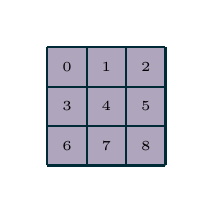
\begin{tikzpicture}[scale=.5,every node/.style={minimum size=1cm}, on grid]
            \draw[fill=base02a,opacity=0.4] (0,0) rectangle (3,3);
            \draw[draw=base03,thick] (0,0) grid (3,3);
            \node (00) at (0.5,2.5) {\tiny 0};
            \node (01) at (1.5,2.5) {\tiny 1};
            \node (02) at (2.5,2.5) {\tiny 2};
            \node (10) at (0.5,1.5) {\tiny 3};
            \node (11) at (1.5,1.5) {\tiny 4};
            \node (12) at (2.5,1.5) {\tiny 5};
            \node (20) at (0.5,0.5) {\tiny 6};
            \node (21) at (1.5,0.5) {\tiny 7};
            \node (22) at (2.5,0.5) {\tiny 8};
    \end{tikzpicture}
\end{figure}

The kernel above, is of size \( \left( \left[ 3, 3 \right] \right) \).
Presenting it as a 4D-Tensor, would give: \( \left( N, C, k_{H}, k_{W} \right)  = \left( \left[ 1, 1, 3, 3 \right] \right)  \)

\subsection*{Stride}
The stride parameter controls the steps in which the kernel 
moves across the input feature map. 
It takes two values, \( \left( \left[ s_{H}, s_{W} \right] \right) \), 
where \( H_{s}, W_{s} \) are the integer step values for the 
height and the width movements across the input feature map.

\begin{figure}[H]
    \centering
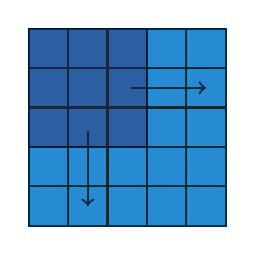
\begin{tikzpicture}[scale=.5,every node/.style={minimum size=1cm}, on grid]
        \begin{scope}[xshift=0,yshift=0cm]
            \begin{scope}[xshift=0cm,yshift=0cm]
                \draw[draw=base03,fill=blue,thick] (0,0) grid (5,5) rectangle (0,0);
                \draw[fill=base02a, opacity=0.4] (0,2) rectangle (3,5);
            \end{scope}
            % \begin{scope}[xshift=7cm,yshift=1.5cm]
            %     \draw[draw=base03,fill=cyan,thick] (0,0) grid (2,2) rectangle (0,0);
            % \end{scope}
        \end{scope}
        \draw[draw=base03, ->, thick] (2.6,3.5) to  (4.5,3.5);
        \draw[draw=base03, ->, thick] (1.5,2.4) to (1.5,0.5);
    % \draw[draw=base03, ->, thick] (5.25, 2.5) to (6.75, 2.5);
    % \begin{scope}[xshift=12cm,yshift=0cm]
    %     \begin{scope}[xshift=0cm,yshift=0cm]
    %         \draw[draw=base03,fill=blue,thick] (0,0) grid (5,5) rectangle (0,0);
    %         \draw[fill=base02, opacity=0.4] (0,2) rectangle (3,5);
    %     \end{scope}
    %     \begin{scope}[xshift=7cm,yshift=1cm]
    %         \draw[draw=base03,fill=cyan,thick] (0,0) grid (3,3) rectangle (0,0);
    %         \draw[draw=base03] (1,0) -- (2,1) -- (2,0) -- (1,1);
    %         \draw[draw=base03] (0,1) -- (1,2) -- (1,1) -- (0,2);
    %         \draw[draw=base03] (1,1) -- (2,2) -- (2,1) -- (1,2);
    %         \draw[draw=base03] (2,1) -- (3,2) -- (3,1) -- (2,2);
    %         \draw[draw=base03] (1,2) -- (2,3) -- (2,2) -- (1,3);
    %     \end{scope}
    %     \begin{scope}[xshift=12cm,yshift=1.5cm]
    %         \draw[draw=base03,fill=cyan,thick] (0,0) grid (2,2) rectangle (0,0);
    %     \end{scope}
    % \end{scope}
    % \draw[draw=base03, ->, thick] (14.6,3.5) to  (15.5,3.5);
    % \draw[draw=base03, ->, thick] (15.6,3.5) to  (16.5,3.5);
    % \draw[draw=base03, ->, thick] (13.5,2.4) to (13.5,1.5);
    % \draw[draw=base03, ->, thick] (13.5,1.4) to (13.5,0.5);
    % \draw[draw=base03, ->, thick] (17.25, 2.5) to (18.75, 2.5);
    % \draw[draw=base03, ->, thick] (22.25, 2.5) to (23.75, 2.5);
    \end{tikzpicture}
    \caption{(a) Mel Filter-Bank representation}
\end{figure}

\begin{figure}[H]
    \centering
    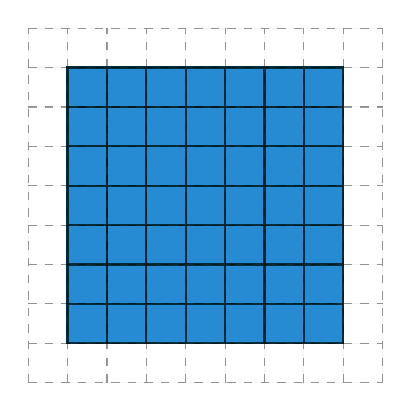
\begin{tikzpicture}[scale=.5,every node/.style={minimum size=1cm}, on grid]
        \tikzmath{
            let \strt = 0;
            let \stp = 7;
        }
        
        \draw[draw=base03,fill=blue,thick] (\strt,\strt) grid (\stp,\stp) rectangle (0,0);
        \draw[fill=base02a, dashed, opacity=0.4] (\strt-1,\strt-1) grid (\stp+1,\stp+1);
        % \draw[fill=base02a, opacity=0.4] (0,2) rectangle (3,5);
        % \draw[draw=base03, ->, thick] (1.5,2.4) to (1.5,0.5);
    \end{tikzpicture}
    \caption{(a) Mel Filter-Bank representation}
\end{figure} 


\begin{figure}[H]
    \centering
    \subfloat[\label{mel_fb_ref}]{
        \centering
        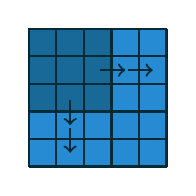
\begin{tikzpicture}[scale=.35,every node/.style={minimum size=1cm},
                            on grid]
            \draw[fill=blue] (0,0) rectangle (5,5);
            \draw[draw=base03, thick] (0,0) grid (5,5);
            \draw[fill=base02, opacity=0.4] (0,2) rectangle (3,5);
            \draw[step=10mm, base03, thick] (0,2) grid (3,5);
            \draw[draw=base03, ->, thick] (2.6,3.5) to  (3.5,3.5);
            \draw[draw=base03, ->, thick] (3.6,3.5) to  (4.5,3.5);
            \draw[draw=base03, ->, thick] (1.5,2.4) to  (1.5,1.5);
            \draw[draw=base03, ->, thick] (1.5,1.4) to  (1.5,0.5);
        \end{tikzpicture}
}
    \subfloat[\label{mel_fb_ref}]{
        \centering
        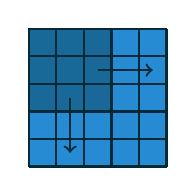
\begin{tikzpicture}[scale=.35,every node/.style={minimum size=1cm},
                            on grid]
            \draw[fill=blue] (0,0) rectangle (5,5);
            \draw[draw=base03, thick] (0,0) grid (5,5);
            \draw[fill=base02, opacity=0.4] (0,2) rectangle (3,5);
            \draw[step=10mm, base03, thick] (0,2) grid (3,5);
            \draw[draw=base03, ->, thick] (2.5,3.5) to  (4.5,3.5);
            \draw[draw=base03, ->, thick] (1.5,2.5) to  (1.5,0.5);
        \end{tikzpicture}
    }
    \caption{(a) Mel Filter-Bank representation}
\end{figure}

\subsection*{Padding}
Padding is a method of extending the input feature map with 
zero values all around in order to control the size dimensions of the 
output feature map. This parameter takes a 2D-Tensor in the form of:
\( \left( \left[ p_{H}, p_{W} \right] \right) \), where \( P_{H}, P_{W} \),
describes the padding depth in the height and width dimensions of the
input feature map.

\begin{figure}[H]
    \centering
    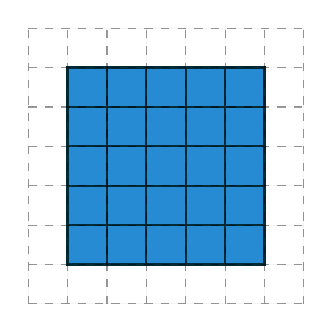
\begin{tikzpicture}[scale=.5,every node/.style={minimum size=1cm}, on grid]
        \draw[draw=base03,fill=blue,thick] (0,0) grid (5,5) rectangle (0,0);
        \draw[fill=base02a, dashed, opacity=0.4] (-1,-1) grid (6,6);
        % \draw[fill=base02a, opacity=0.4] (0,2) rectangle (3,5);
        % \draw[draw=base03, ->, thick] (1.5,2.4) to (1.5,0.5);
    \end{tikzpicture}
    \caption{(a) Mel Filter-Bank representation}
\end{figure}

\subsection*{Dilation}
Dilation represents the integer spaces placed between the kernel elements.
For a given dilation value \(d\),
the elements of the kernel are spaced with \(d - 1\) in between.

This parameter takes a 2D-Tensor in the form of:
\( \left( \left[ d_{H}, d_{W} \right] \right) \),
where \( d_{H}, d_{W} \),
describes the \(d - 1 \) spaces in between kernel elements. 

\begin{figure}[H]
    \centering
    \subfloat[\label{conv2d_dil1}]{
        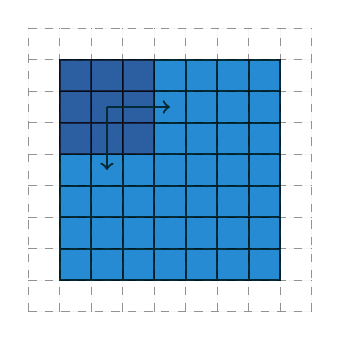
\begin{tikzpicture}[scale=.4,every node/.style={minimum size=1cm}, on grid]
            
            \draw[draw=base03,fill=blue,thick] (0,0) grid (7,7) rectangle (0,0);
            \draw[fill=base02a, dashed, opacity=0.4] (-1,-1) grid (8,8);

            \foreach \x in {0,1,2} {
                \foreach \y in {4,5,6} {
                    \draw[fill=base02a, opacity=0.4] (\x,\y) rectangle (\x+1,\y+1);
                    % \node at (\x,\y) [circle,fill=black] {};
                    %this way circle of nodes will not be transformed
                }
            }
            % \draw[draw=base03, ->, thick] (2.5,2.4) to (2.5,0.5);
            \draw[draw=base03, ->, thick] (1.5,5.5) to  (3.5,5.5);
            \draw[draw=base03, ->, thick] (1.5,5.5) to  (1.5,3.5);
        \end{tikzpicture}
    }
    \subfloat[\label{conv2d_dil2}]{
        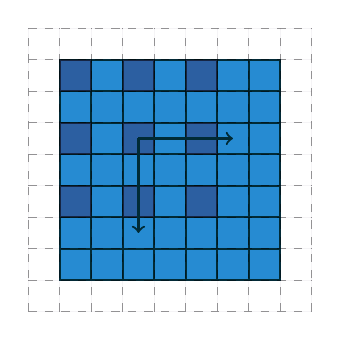
\begin{tikzpicture}[scale=.4,every node/.style={minimum size=1cm}, on grid]
            \draw[draw=base03,fill=blue,thick] (0,0) grid (7,7) rectangle (0,0);
            \draw[fill=base02a, dashed, opacity=0.4] (-1,-1) grid (8,8);

            \foreach \x in {0,2,4} {
                \foreach \y in {2,4,6} {
                    \draw[fill=base02a, opacity=0.4] (\x,\y) rectangle (\x+1,\y+1);
                    % \node at (\x,\y) [circle,fill=black] {};
                    %this way circle of nodes will not be transformed
                }
            }
            % \draw[draw=base03, ->, thick] (2.5,2.4) to (2.5,0.5);
            \draw[draw=base03, ->, thick] (2.5,4.5) to  (5.5,4.5);
            \draw[draw=base03, ->, thick] (2.5,4.5) to  (2.5,1.5);
        \end{tikzpicture}
    }
    % \subfloat[\label{conv2d_dil3}]{
    %     \begin{tikzpicture}[scale=.4,every node/.style={minimum size=1cm}, on grid]
    %         \draw[draw=base03,fill=blue,thick] (0,0) grid (9,9) rectangle (0,0);
    %         \draw[fill=base02a, dashed, opacity=0.4] (-1,-1) grid (10,10);

    %         \foreach \x in {0,3,6} {
    %             \foreach \y in {2,5,8} {
    %                 \draw[fill=base02a, opacity=0.4] (\x,\y) rectangle (\x+1,\y+1);
    %             }
    %         }
    %         \draw[draw=base03, ->, thick] (3.5,5.5) to  (5.5,5.5);
    %         \draw[draw=base03, ->, thick] (3.5,5.5) to  (3.5,3.5);
    %     \end{tikzpicture}
    % }
    \caption{(a) Mel Filter-Bank representation}
\end{figure}

\subsubsection{Convolutional Layer Output}
A convolutional layer,
after convolving a kernel with an input tensor,
outputs a feature map. The output feature map dimensions
are set by the different parameters of the convolutional layer.

The padding \( p_{H}, p_{W} \) increases the height and width of 
the output feature map, while the stride \( s_{H}, s_{W} \) 
and dilation \( d_{H}, d_{W} \) shrink it.

\begin{align}
    H_{out} =& \left\lfloor\frac{H_{in}  + 2 \times p_{_{H}} - d_{_{H}}
                        \times (k_{_{H}} - 1) - 1}{s_{_{H}}} + 1\right\rfloor  \\
    W_{out} =& \left\lfloor\frac{W_{in}  + 2 \times p_{_{W}} - d_{_{W}}
                        \times (k_{_{W}} - 1) - 1}{s_{_{W}}} + 1\right\rfloor
\end{align}

\begin{figure}[H]
    \centering
    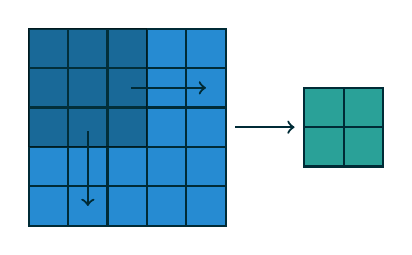
\begin{tikzpicture}[scale=.5,every node/.style={minimum size=1cm}, on grid]
        \begin{scope}[xshift=0,yshift=0cm]
            \begin{scope}[xshift=0cm,yshift=0cm]
                \draw[draw=base03,fill=blue,thick] (0,0) grid (5,5) rectangle (0,0);
                \draw[fill=base02, opacity=0.4] (0,2) rectangle (3,5);
            \end{scope}
            \begin{scope}[xshift=7cm,yshift=1.5cm]
                \draw[draw=base03,fill=cyan,thick] (0,0) grid (2,2) rectangle (0,0);
            \end{scope}
        \end{scope}
        \draw[draw=base03, ->, thick] (2.6,3.5) to  (4.5,3.5);
        \draw[draw=base03, ->, thick] (1.5,2.4) to (1.5,0.5);
        \draw[draw=base03, ->, thick] (5.25, 2.5) to (6.75, 2.5);
    \end{tikzpicture}
    \caption{(a) Mel Filter-Bank representation}
\end{figure}



\subsection{Recurrent Layers}
\subsubsection{LSTM}
\subsubsection{BLSTM}
\subsubsection{RNN}

\subsection{Transformer Layers}
\subsubsection{Transformer}
\subsubsection{Transformer-Encoder}
\subsubsection{Transformer-Decoder}


\section{NN Function Layers}
\subsection{Non-linear Activations Functions}
\subsubsection{ReLU}


\subsubsection{LeakyReLU}


\subsubsection{Sigmoid}
\subsubsection{Tanh}
\subsubsection{Softplus}

\subsection{Normalization Functions}
\subsubsection{Batch-Normalization}

\subsection{Pooling Functions}
\subsubsection{Min-pooling}
\subsubsection{Average-pooling}
\subsubsection{Max-pooling}

\section{Dropout Layers}
\subsubsection{p-Dropout}
To avoid some redundant feature\((s)\) detection by multiple neurons in a network,
a co-adaptation amongst the different neurons in the model should be prevented. 
In that way, the NN model is much more effective and uses resources more efficiently.

This holds true especially during training, as described in this paper
\citep{hinton2012improving}.

The idea is to zero-out, arbitrarily, values of
the input feature. 
Based on the \emph{Bernoulli distribution}, the probability to zero an element gets the
probability \(p\), while the opposite, non-zeroing probability is set to \(1-p\). 

Raising the \(p\) value too high, may lead to an exhaustive training process, thus 
a good balance point should be used to overcome the co-adaptation while not missing 
useful features. Whenever the training sets are considered large, a small portion 
of zeroed elements should be sufficient for satisfactory results.  

\subsection{Loss Functions}
\subsubsection{L1 Loss (MAE)}
\subsubsection{L2 Loss (MSE)}
\subsubsection{Cross-Entropy}
\subsubsection{CTC}
% \chapter{Experiments}
\section{T-F Masking Estimations}
\subsection{IRM}

\subsection{cIRM}

\begin{figure}[H]
    \centering
    \includegraphics[width=0.75\linewidth]{Features/images/cIRM_real_mask}
    \caption{cIRM real mask}\label{fig:asr_5}
\end{figure}

\begin{figure}[H]
    \centering
    \includegraphics[width=0.75\linewidth]{Features/images/cIRM_imag_mask}
    \caption{cIRM imag mask}\label{fig:asr_5}
\end{figure}

\subsection{PSM}
\begin{figure}[H]
    \centering
    \includegraphics[width=0.75\linewidth]{Features/images/psm_mask}
    \caption{psm mask}\label{fig:asr_5}
\end{figure}

\subsection{ORM}
\begin{figure}[H]
    \centering
    \includegraphics[width=0.75\linewidth]{Features/images/orm_mask}
    \caption{orm mask}\label{fig:asr_5}
\end{figure}


\begin{table}[H]
    % for more info see: https://www.overleaf.com/learn/latex/tables
    \centering
    % \hspace*{-2.8cm}
    \arrayrulecolor{mtblborder}
\begin{tabular}{ !{\color{mtblborder}\vrule}c!{\color{mtblborder}\vrule}cc|||cc| } 
    \hline

    \hline
    \rowcolor{mtblcaption}
    & \multicolumn{2}{c}{\color{white}\bf{Learnable Parameters} [Mil]}
    & \multicolumn{2}{c}{\color{white}\bf{Quant. (S16.11) Mem } [Mb]}\\         
    % \cline{2-8}
    
    \multirow{-2}{*}{\cellcolor{mtblcaption}\color{white}\bf{Targets} }
    & \cellcolor{mtbl} \color{black}{W/o (\(\Delta\),\(\Delta\Delta\))} 
    & \cellcolor{mtbl} \color{black}{W/ (\(\Delta\),\(\Delta\Delta\))}
    & \cellcolor{mtbl} \color{black}{W/o (\(\Delta\),\(\Delta\Delta\))} 
    & \cellcolor{mtbl} \color{black}{W (\(\Delta\),\(\Delta\Delta\))} \\
    % & \color{white}\bf{ORM} 
    % & \color{white}\bf{Clean} \\
    \hline

    \hline
    \rowcolor{mtblA} IRM  
        & 2.44 
        & 4.67
        & 39.0
        & 74.8 \\
    \hline
    
    \hline
    \rowcolor{mtbl} cIRM  
        & 3.76
        & 5.99
        & 60.1
        & 95.9 \\
    \hline

    \hline
    \rowcolor{mtblA} PSM  
        & 3.49
        & 5.73
        & 55.9
        & 91.7 \\
    \hline

    \hline
    \rowcolor{mtbl} ORM  
        & 3.50
        & 5.74
        & 56.0
        & 91.8 \\
    \hline
    
    \hline
\end{tabular}
\arrayrulecolor{black}
\caption{T-F Masks models learnable parameters vs. Required memory size}
\label{tbl:masks_l_params}
\end{table}


\section{Front-End Beamformers}
\subsection{IRM Beamformer}
\begin{figure}[H]
    \centering
    \includegraphics[width=\linewidth]{Experiments/images/irm_pesq_mosq}
    \caption{IRM beamformer PESQ vs. MOSLQ}\label{fig:irm_pesq_mosq}
\end{figure}

\begin{table}[H]
    % for more info see: https://www.overleaf.com/learn/latex/tables
    \centering
    \begin{tabular}{lr}
      \midrule
      Set & Utterances [\(N\)] \\
      \midrule
        Training    & 759,546   \\
        Dev/Valid   & 16,264   \\
        Test        & 16,236  \\
       \bottomrule
    \end{tabular}
    \caption{IRM beamformer PESQ \& MOSLQ}\label{tbl:comvoice_set_dstrb}
\end{table}

\subsection{cIRM Beamformer}
\begin{figure}[H]
    \centering
    \includegraphics[width=\linewidth]{Experiments/images/irm_pesq_mosq}
    \caption{IRM beamformer PESQ vs. MOSLQ}\label{fig:cirm_pesq_mosq}
\end{figure}

% \section{Engines}




% \subsection{FB Transformer}

% \subsection{MFCC Transformer}

% \subsection{RFCC Transformer}
% kldiv loss = seqloss
% ctc loss

% \begin{equation}
%     \ell = \omega_{_{ctc}}  \ell_{_{ctc}} + (1 - \omega_{_{ctc}}) \cdot \ell_{_{seq}}
% \end{equation}




% \chapter{Scaling methods}



% \begin{table}
%     \centering
%     \begin{tabular}
%         {!{\color[HTML]{00638a}\vrule}l
%         !{\color[HTML]{00638a}\vrule}l
%         llllll
%         !{\color[HTML]{00638a}\vrule}}
%         \arrayrulecolor[HTML]{00638a}\hline
%         \rowcolor[rgb]{0.6,0.757,0.945}  &                                    &                                    &                                    &                                    &                                    &                                    &                                     \\ 
%         \arrayrulecolor[HTML]{00638a}\cline{2-8}
%         \multirow{-2}{*}{{\cellcolor[rgb]{0.6,0.757,0.945}}}               &                                    &                                    &                                    &                                    &                                    &                                    &                                     \\ 
%         \arrayrulecolor[HTML]{00638a}\hline
%         \multirow{2}{*}{}                                                  & {\cellcolor[rgb]{0.6,0.757,0.945}} & {\cellcolor[rgb]{0.6,0.757,0.945}} & {\cellcolor[rgb]{0.6,0.757,0.945}} & {\cellcolor[rgb]{0.6,0.757,0.945}} & {\cellcolor[rgb]{0.6,0.757,0.945}} & {\cellcolor[rgb]{0.6,0.757,0.945}} & {\cellcolor[rgb]{0.6,0.757,0.945}}  \\ 
%         \arrayrulecolor[HTML]{00638a}\cline{2-8}
%                                                                        &     
%                                                                     &                                    &                                    &                                    &                                    &                                    &   \\ 
%         \arrayrulecolor[HTML]{00638a}\hline
%     \end{tabular}
%     \arrayrulecolor{black}
%     \end{table}


% \begin{table}[H]
%     % for more info see: https://www.overleaf.com/learn/latex/tables
%     \centering
%     \arrayrulecolor[HTML]{00638a}
% \begin{tabular}{ !{\color[HTML]{00638a}\vrule}c!{\color[HTML]{00638a}\vrule}ccccccc| } 
%     \hline

%     \hline
%     \rowcolor[HTML]{00a5ef} \color{white}\bf{Id} & \color{white}\bf{ASR Tr.} & \color{white}\bf{Noisy} & \color{white}\bf{IRM} & \color{white}\bf{cIRM} & \color{white}\bf{PSM} & \color{white}\bf{ORM} & \color{white}\bf{Clean} \\
%     \hline

%     \hline
%     \rowcolor[HTML]{ddf4ff}                         & 28.62/32.02 & 46.19 & 27.78 & - & - & - & 17.55 \\
%     \cline{2-8}
%     \multirow{-2}{*}{\cellcolor[HTML]{ddf4ff}\#1(5)}   & 14.03/17.78 & 27.06 & 13.73 & - & - & - & 7.72 \\ 
%     \hline

%     \hline
%     \rowcolor[HTML]{ddf4ff}\cellcolor[HTML]{ffffff} & 28.38/31.61 & - & - & - & - & - & - \\
%     \cline{2-8}
%     \multirow{-2}{*}{\#2(15)}                           & 13.27/16.68 & - & - & - & - & - & - \\ 
%     \hline
    
%     \hline
%     \rowcolor[HTML]{ddf4ff}                         & 28.09/31.18 & 46.25 & 28.03 & - & - & - & 18.46 \\
%     \cline{2-8}
%     \multirow{-2}{*}{\cellcolor[HTML]{ddf4ff}\#3(12)}   & 13.28/16.53 & 26.56 & 13.35 & - & - & - & 7.39 \\ 
%     \hline

%     \hline
%     \rowcolor[HTML]{ddf4ff}\cellcolor[HTML]{ffffff} & 28.77/31.6 & - & - & - & - & - & - \\
%     \cline{2-8}
%     \multirow{-2}{*}{\#4(22)}                           & 14.06/16.42 & - & - & - & - & - & - \\ 
%     \hline
    
%     \hline
%     \rowcolor[HTML]{ddf4ff}                         & 28.92/32.32 & - & - & - & - & - & - \\
%     \cline{2-8}
%     \multirow{-2}{*}{\cellcolor[HTML]{ddf4ff}\#5(23)}   & 13.53/17.05 & - & - & - & - & - & - \\ 
%     \hline

%     \hline
%     \rowcolor[HTML]{ddf4ff}\cellcolor[HTML]{ffffff} & 28.29/31.50 & - & - & - & - & - & - \\
%     \cline{2-8}
%     \multirow{-2}{*}{\#6(70)}                           & 13.42/16.72 & - & - & - & - & - & - \\ 
%     \hline
    
%     \hline
%     \rowcolor[HTML]{ddf4ff}                         & 28.26/31.51 & - & - & - & - & - & - \\
%     \cline{2-8}
%     \multirow{-2}{*}{\cellcolor[HTML]{ddf4ff}\#7(72)}   & 13.14/16.53 & - & - & - & - & - & - \\ 
%     \hline

%     \hline
%     \rowcolor[HTML]{ddf4ff}\cellcolor[HTML]{ffffff} & 29.60/35.00 & 45.79 & 28.07 & - & - & - & 19.23 \\
%     \cline{2-8}
%     \multirow{-2}{*}{\#8(100)}                           & 13.57/17.38 & 25.76 & 12.97 & - & - & - & 7.61 \\ 
%     \hline

%     \hline
%     \rowcolor[HTML]{ddf4ff}                         & 29.46/32.06 & 46.71 & 28.51 & - & - & - & 18.79 \\
%     \cline{2-8}
%     \multirow{-2}{*}{\cellcolor[HTML]{ddf4ff}\#9(13)}   & 14.16/17.77 & 26.59 & 14.03 & - & - & - & 7.84 \\ 
%     \hline

%     \hline
% \end{tabular}
% \arrayrulecolor{black}
% \caption{\bf{ IQRD Performance:} Latency and Resource Utilization vs Channel Count for XCZU3EG FPGA}
% \label{tbl:IQRD_perf}
% \end{table}
% \begin{table}[H]
%     % for more info see: https://www.overleaf.com/learn/latex/tables
%     \centering
%     \begin{tabular}{|c|r|r|r|r|r|}
%       \hline
%       Id & ASR Tr. & FF & LUT & DSP48 & BRAM \\
%       \hline
%       \multirow{2}3  & 4.80  &   3889 (27.6\%) &    3901 (54.9\%) &   90 (25.0\%) & 0 (0.0\%) \\
%       & 4.80  &   3889 (27.6\%) &    3901 (54.9\%) &   90 (25.0\%) & 0 (0.0\%) \\
%         4  & 6.34  &  63657 (45.1\%)                 &   64149 (90.4\%)                  &  144 (40.0\%) & 0 (0.0\%) \\
%         8  & 12.50 & 231199 (\textcolor{red}{164\%}) &  252446 (\textcolor{red}{356\%})  &  272 (75.6\%) & 0 (0.0\%) \\
%         16 & 24.82 & 895377 (\textcolor{red}{635\%}) & 1040992 (\textcolor{red}{1466\%}) &  144 (40.0\%) & 0 (0.0\%) \\
%        \hline
%     \end{tabular}
%     \caption{\bf{ IQRD Performance:} Latency and Resource Utilization vs Channel Count for XCZU3EG FPGA}
%     \label{tbl:IQRD_perf}
% \end{table}





\end{document}
